\chapter{保护}
\section{引言}
保护是五大关键设计和运行项目之一---其他四项是稳定性、机械完整性、制冷和导体。
如图1.6中定性给出的,随着运行温度提高,磁体保护的难度或成本增加,而稳定性的实现难度或成本降低。
如第6章所述,对于HTS磁体,尽管其稳定性很好,但保护可能成为一个真正的挑战。
关于HTS磁体保护最长问到的问题是:“既然HTS磁体如此稳定,为何要担心它的保护?”
答案归结为HTS设备的成本及其保护成本两者的权重,以及待保护系统出现故障的可能性。
对“固有稳定”的HTS磁体,保护还是不保护,是一个难题。这个问题在讨论8.7中再次讨论。

我们的重点是保护磁体绕组;磁体的的其他部分---机械的,电的和低温的---略过不谈。
本章包括的问题是:1)过热; 2)应力(热的和机械的); 3)内部高电压; 4)保护技术。
专题部分还涉及其他主题。
保护当然是超导磁体的一个关键主题,自1960年代以来,一些已经得到解决[1.27,8.1-8.6],一些得到更新升级[8.7-8.11];
其他参考文献在适当的时候引用。

\subsection{热能密度 vs. 磁能密度}
除非绕组得到了保护,不然磁体绕组的一小部分,即“热点”,就要吸收掉存储于绕组中的大部分磁能。这样,该部分将过热并永久性损坏。
不过,熔化磁体中单位绕组体积的热能密度要远大于磁体存储的磁能密度。

仅考虑将磁体内部空间内存储的能量全部绝热转换为热,引起铜(绕组的一种代表性材料)的焓密度$h_{Cu}(T)$变化。如果是从4K(或者80K)加热到它的熔点1356K,那么初始磁感应密度$B_0$将高达$~150 T$:
\begin{equation}% 8.1第一个
\frac{B_{0}^{2}}{2\mu_o}=h_{cu}(1356\ \mathrm{K})-h_{cu}(4\ \mathrm{K}\ \mathrm{or}80\ \mathrm{K})\simeq 5.2\times 10^9\ \mathrm{J/m^3}
\end{equation}
\begin{align*}% 8.1第二个
B_0\simeq\sqrt{2(4\pi\times 10^{-7}\ \mathrm{H/m})(5.2\times 10^9\ \mathrm{J/m^3})}\simeq 115\ \mathrm{T}
\end{align*}

即便是不很大的磁体(如3 T)也会由于过热而永久损坏,表明了灾难性的能量集中确实可能发生于\textit{真实}磁体中。
如果仅将局域的磁能密度局部转换为局域的热,使用类似8.1的方法用焓密度计算场能量密度,得到小于$\sim$25 T的磁场,温度低于200 K;
对于大于$\sim$25 T的情,参见下一节中的实例。

\subsection{热点和热点温度}
磁体失超通常开始于很小的绕组体积(所谓的热点)内。
如上所述,磁体的全部存能会在该热点上耗散,导致磁体的永久性损坏。

这里,我们研究存储在螺线管中的全部磁能$E_m$在热点中的绝热吸收,以及所对应的热点最终温度$T_f$。
磁体保护的目标是将$T_f$限制在$\sim$200 K以下,绝不能高于300 K。
自感为$L$的螺线管在电流I下存储的磁能$E_m$由下式给出:
\begin{align*}% page468 3.79
E_m=\frac{1}{2}LI^2 \tag{3.79}
\end{align*}

方程3.81给出了总匝数为$N$的螺管线圈$(a_1,\alpha,\beta)$的电感$L$:
\begin{align*}% page468 3.81
L=\mu_oa_1\ \mathcal{L}(\alpha,\beta)N^2 \tag{3.81}
\end{align*}

图3.14给出了仅依赖于绕组参数$\alpha$和$\beta$的$\mathcal{L}(\alpha,\beta)$。轴向中心场$B_o$为:
\begin{equation}% 8.2
B_o=\frac{\mu_oNI}{2a_1(\alpha-1)\beta}F(\alpha,\beta)
\end{equation}
其中,$F(\alpha,\beta)$为:
\begin{align*}% page468 3.13b
F(\alpha,\beta)=\beta\left(\frac{\alpha+\sqrt{\alpha^2+\beta^2}}{1+\sqrt{1+\beta^2}}\right) \tag{3.13b}
\end{align*}

由8.2,我们可以用$a_1,\alpha,\beta,B_o$来表示$NI$:
\begin{equation}% 8.3
NI=\frac{2a_1(\alpha-1)\beta B_o}{\mu_oF(\alpha,\beta)}
\end{equation}

这样,对一个参数为$\alpha,\beta$的螺管,它的与$B_o$有关的磁场能量密度$E_m$为:
\begin{equation}% 8.4
E_m=\frac{4a_{1}^{3}(\alpha-1)^2\beta^2\ \mathcal{L}(\alpha,\beta)}{F^2(\alpha,\beta)}\left(\frac{B_{o}^{2}}{2\mu_o}\right)
\end{equation}

总绕组体积$V_w$由下式给出:
\begin{equation}% 8.5
V_w=2\pi a_{1}^{3}(\alpha^2-1)\beta
\end{equation}

注意,$V_m$包括所有绕组材料,既包括导体也包括非导体。总的热点(电阻区域)体积$V_r$为:
\begin{equation}% 8.6
V_r=f_eV_w=f_r2\pi a_{1}^{3}(\alpha^2-1)\beta
\end{equation}
其中,$f_r$是热点体积占绕组的比分。
如果磁体的总磁场能量$E_m$绝热的转换为热点内的热,
热点的平均热能密度$e_{mr}$为:
\begin{equation}% 8.7
e_{mr}=\frac{E_m}{V_r}=\frac{2(\alpha-1)\beta\ \mathcal{L}(\alpha,\beta)}{f_r\pi(\alpha+1)F^2(\alpha,\beta)}\left(\frac{B_{o}^{2}}{2\mu_o}\right)
\end{equation}

$e_{mr}$不依赖于磁体体积,而是依赖于$f_r,\alpha,\beta$和$B_o$。
不过,实际需要的用以限制其温度$T_f$的热点体积随绕组体积增大而增加。
在螺管磁体中以最小化热点体积实现$T_f\le 200$ K的要求是保护的一个关键问题:
这将在下文的实例中讨论。

表8.1.。。。。。。。。。。。。。。。。。。

\textbf{实例}\quad 表8.1给出了螺管线圈($\alpha,\beta$)在磁场$B_o$=1.5-30 T区间运行,为了限制最高
热点温度$T_f$为200 K和300 K所要求的的热点体积分数$f_r\%$。初始绕组温度$T_i$有两种,4 K和80 K。
这里,假定绕组全部是铜(密度$8.96\ \mathrm{g/cm^3}$),$T_f$采用$e_{mr}=h_{cu}(T_f)-h_{cu}(T_i)$计算,
其中$e_{mr}$如8.6所给。
这个表给出,这个螺管($\alpha=1.5,\beta=2.0$)产生1.5 T的磁场,为了限制$T_f$为200 K和300 K,所需的热点
分数只是绕组体积的很小一部分(<1\%)。
实现$T_f\le 200$ K只需很小体积分数的事实对“检测-激活加热器”主动保护有很好的实践意义:
对多数螺管线圈,如8.8.4中所讨论的,需要在绕组内部放置一个很笨重的“保护加热器”将很小的一部分绕组转换(扩大)为
热点。不过,从表8.1明显可见,尽管在螺管的$B_o$小于25 T时$f_r\le 1$;但对$B_o\ge 30$ T,$f_r$将超过1,
即储存的磁能的一部分必须在螺管外耗散,比如进入保护电阻(8.8.3)。

\subsection{绕组材料的温度数据}
表8.2列出了LTS和HTS磁体常用绕组材料允许的热点温度$T_f$极限,下面对其中的内容简要讨论。
\begin{description}
	\item[200 K之下] 人们普遍认为,在电阻区,哪怕仅局限于绕组体积的很小一部分,也可被加热到200 K。
	因为绕组中部分为200 K,其余部分为低至4.2 K的初始温度下的热应变差别小于$\sim 0.1\%$,这
	对于大多数磁体级超导体导体是安全的。
	\item[320 K] Indium合金的最低熔点。
	\item[335 K] Cu加强YBCO样品($I_c$=161 A@77.3 K)由60 ms的1.23 kA电流脉冲加热后,$I_c$无退化。
	\item[370 K] 与上一项相同的样品,经过60 ms的1.36 kA电流脉冲加热后,$I_c$轻微退化(161 A$\rightarrow$157 A)。
	\item[380 K] 超过这个温度,绕组中常用的有机材料Formvar绝缘和Stycast2850失效。
	\item[400 K和430 K] 约400 K,paraffin熔化;430 K,铟熔化。
	\item[456 K] 磁体中广泛使用的焊料63Sn-37Pb熔化。
	\item[720 K] Bi2223-Ag测试样品($I_c$=119 A@77.3 K)由320 ms的450 A电流脉冲加热后,$I_c$无退化。
	\item[800 K] 同样的Bi带样品,由330 ms的450 A脉冲电流加热后,$I_c$明显退化(119 A$\rightarrow$50 A)。
\end{description}

表8.2.。。。。。。。。。。。。。。

\subsection{安全、风险和高度风险$T_f$区间}
我们可以将上述温度分为三个$T_f$区域用于绕组:1)安全区间; 2)有风险区间; 3)高风险区间。

\begin{description}
	\item[安全区间] 对正常区域,$T_f$低于200 K是安全的上限。
	LTS和HTS绕组之间在这方面没有基本差异。
	不过,在某些应用中,恢复到正常工作温度的时间很重要,所以希望较低的$T_f$。
	\item[风险区间] 200-300 K的范围是需要“小心的”。
	如果$T_f$保持在该区间,除了热应力存在风险,没有绕组材料被加热到高度危险并因此受损的地步。
	\item[高风险] 无论是LTS还是HTS绕组,$T_f$高于300 K都是高风险的。
\end{description}

\subsection{温度引起的应力}
过热除了引起绕组热损伤,还可能通过应变引起绕组的机械损伤。
表8.3给出了几种磁体绕组材料在293 K时的线性热膨胀(事实是,收缩)数据,$[L(T)-L(293\ \mathrm{K})]/L(293\ \mathrm{K})$。
考虑一个饼式线圈,并假设线圈的内半部分加热到140 K,而外半部分保持在80 K。
表8.3中的数据表明在外半部分最内层引起的拉伸应变不会超过$\sim 0.1\%$,这应该是安全的。
如果线圈的内半部分被加热到300 K,而外半部分保持在80 K,那么引起的应变可能超过$0.2\%$,这对Nb3Sn和HTS达到了危险水平。
不过,即使在加热过程中保持温度均匀,由于磁体绕组由具有不同热膨胀系数的材料组成(表8.3),
均匀加热仍会在超导体中引起应力。将$T_f$保持在200 K以下通常是最安全的。

表8.3.。。。。。。。。。。。。。。。


\section{绝热加热}
超导磁体中永久性损坏的主要形式之一是其复合导体的过度加热(“过热”)。
如果严重,过热可能会使复合材料熔化或在绕组中产生热梯度,在超导体内形成过应力,不可逆地降低其$J_c$性能。
1960年代以来,过热问题得到了实验和分析的研究。

如上所述,即使磁体与其电源隔离并且以持续模式运行,超导磁体中的过热仍可能通过在磁体中存储的总磁能在绕组的小体积内耗散而发生。
在带电磁体中,在磁体被驱动到正常态后,电源的电阻性加热也可能发生过热;
这种加热可以是局域的,也可能是包括整个绕组的全局的。
忽略方程6.1中的热传导、扰动和冷却项,我们来分析单位复合导体体积的绝热加热。
\begin{subequations}
	\begin{align}
	C_{cd}(T)\frac{dT}{dt}&\simeq\rho_{cd}(T)J_{cd_o}^{2}(t) \\
	&\simeq\rho_m(T)J_{cd_o}^{2}(t)
	\end{align}
\end{subequations}

方程8.8b中,如图6.5的电路模型一样,导体的电阻率$\rho_{cd}$由基底电阻率$\rho_m$近似(或方程6.25的$n=\infty$)。
注意到,方程8.8出现在第六章表6.1的第七行。

\subsection{恒定电流模式下的绝热加热}
首先我们研究图如8.1所示的恒电流模式的绝热加热:
超导磁体(电感$L$)内的电阻性区域$r(T)$与提供磁体运行电流$I_{op}$的恒流源相连。
假设电阻性区域如8.8b载有\textit{全部}电流,单位导体长度的功率密度方程称为:
\begin{equation}% 8.9a
A_{cd}C_{cd}(T)\frac{dT}{dt}=\frac{\rho_m(T)}{A_m}I_{op}^{2}(t)
\end{equation}
代入$I_{op}/A_m=J_m$(方程6.7c),以及$C_{sc}(T)\simeq C_{\bar{m}}(T)\simeq C_m(T)$,$A_m/A_{cd}=\gamma_{m/s}/(\gamma_{m/s}+1)$(其中,$\gamma_{m/s}\equiv A_m/(A_{sc}+A_{\bar{m}})$,方程6.21b),
得到:
\begin{align*}% 8.9b
C_m(T)\frac{dT}{dt}=\left(\frac{A_m}{A_{cd}}\right)\rho_m(T)J_{m_o}^{2}=\left(\frac{\gamma_{m/s}}{1+\gamma_{m/s}}\right)\rho_m(T)J_{m_o}^{2} \tag{8.9b}
\end{align*}
整理8.9b,在初始值($t=0$时,$T=T_i$)和最终值($t=\tau_{ah}$时,$T=T_f$),有:
\begin{align*}% 8.9c和8.9d
\int_{T_i}^{T_f}\frac{C_m(T)}{\rho_m(T)}dT=\left(\frac{A_m}{A_{cd}}\right)J_{m_o}^{2}\tau_{ah} \tag{8.9c}
\end{align*}
\begin{align*}
\int_{T_i}^{T_f}\frac{C_m(T)}{\rho_m(T)}dT=\left(\frac{\gamma_{m/s}}{1+\gamma_{m/s}}\right)J_{m_o}^{2}\tau_{ah} \tag{8.9d}
\end{align*}

方程8.9c和8.9d左侧的温度积分单调的依赖于$T$;我们定义$Z(T_f,T_i)$函数:
\begin{equation}% 8.10a
Z(T_f,T_i)\equiv\int_{T_i}^{T_f}\frac{C_m(T)}{\rho_m(T)}dT
\end{equation}
对于$\rho_m(T)$比较恒定的合金基底金属,可用温度区间平均值$\tilde{\rho}_m$近似替代,方程8.10可以简化为:
\begin{align*}% 8.10b
Z(T_f,T_i)\simeq\frac{1}{\tilde{\rho}_m}\int_{T_i}^{T_f}C_m(T_f)dT=\frac{H_m(T_f)-H_m(T_i)}{\tilde{\rho}_m}\tag{8.10b}
\end{align*}
其中,$H_m(T)$是温度$T$时基地金属单位体积焓。

\begin{figure}
	\centering
	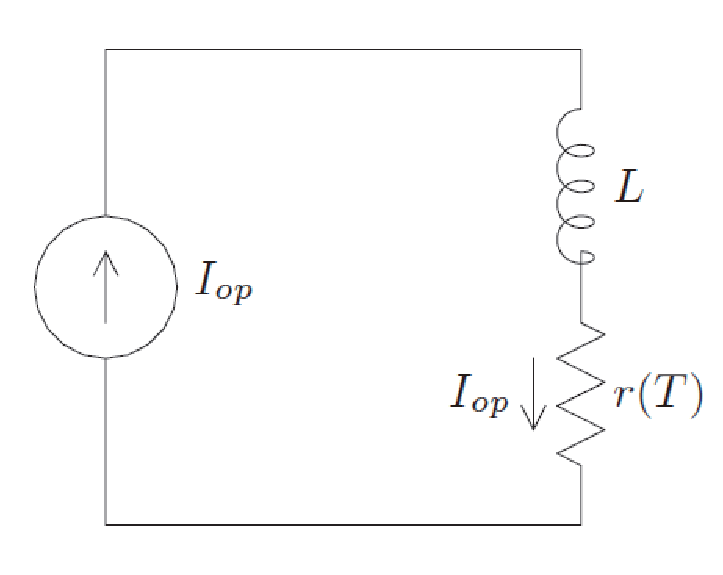
\includegraphics[scale=0.5]{chpt8/figs/fig8.1.eps}
	\caption{电路模型:电感为$L$的超导磁体,有依赖于温度的正常区电阻$r(T)$,连基于恒流$I_{op}$源。}
\end{figure}
图8.2给出了银(0$^\circ$C和4$^\circ$C的电阻率RRR=1000;100)、铜(200;100;50)、铝(级别:1000)和黄铜(70Cu-30Zn)的$Z(T,0)$。
虚线(不易看出)是$\tilde{\rho}_m=5.5\times 10^{-8}\Omega$m(方程8.10b)的黄铜。对任意的$T_i,T_f$组合,有:
\begin{equation}% 8.11
Z(T_f,T_i)=Z(T_f,0)-Z(T_i,0)=Z(T_f)-Z(T_i)
\end{equation}
对任意的$T_i,T_f$组合,存在一个加热时间$\tau_{ah}^i(T_f,T_I)$---
角标$i$表示恒电流加热---有下式给出:
\begin{equation}% 8.12a
\tau_{ah}^{i}(T_f,T_i)=\left(\frac{1+\gamma_{m/s}}{\gamma_{m/s}}\right)\frac{Z(T_f,T_i)}{J_{m_o}^{2}}
\end{equation}
类似的,对任意的$T_i,T_f$组合,在恒电流加热时间$\tau_{ah}$内存在一个基底电流密度$J_{m_o}^i(T_f,T_i)$:
\begin{align*}% 8.12b
J_{m_o}^{i}(T_f,T_i)=\sqrt{\left(\frac{1+\gamma_{m/s}}{\gamma_{m/s}}\right)\frac{Z(T_f,T_i)}{\tau_{ah}}} \tag{8.12b}
\end{align*}

因为在$\sim 300$ K以上,$C_m(T)$存在渐近线,而$\rho_m(T)$却继续随$T$增长。被积函数$C_m(T)/\rho_m(T)$随$T$减小,
所以$Z(T_f,T_i)$的很小增量会引起(多数实际损坏的)绕组$T_f$的剧烈增加:保持$T_f$不大于200 K。

\begin{figure}
	\centering
	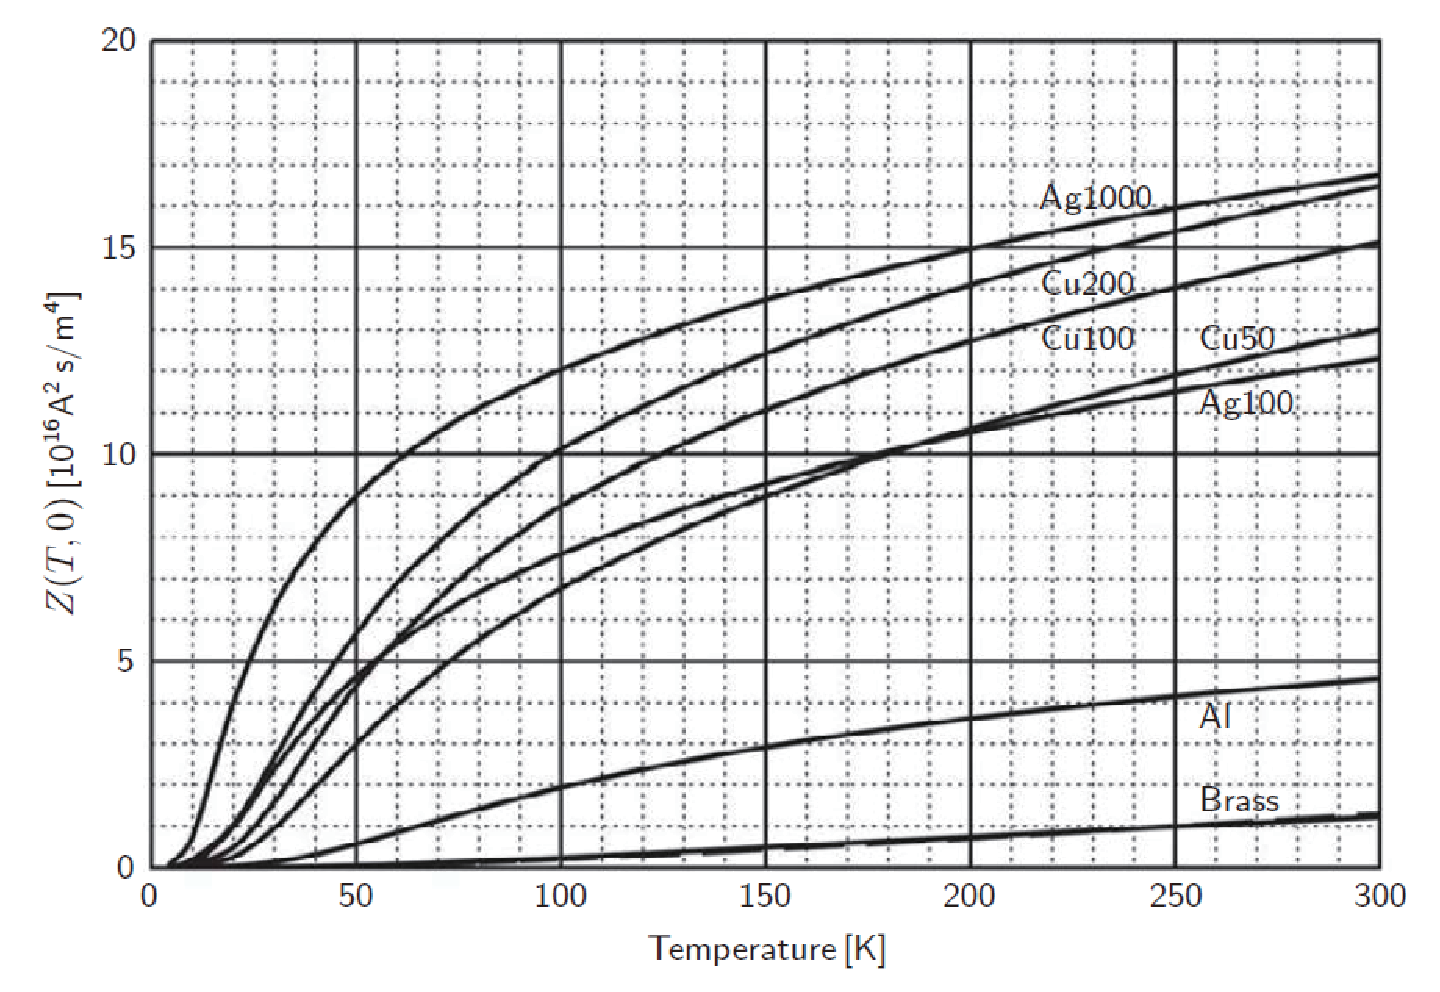
\includegraphics[scale=0.5]{chpt8/figs/fig8.2.eps}
	\caption{几种常用金属材料的$Z(T, 0)$图。}
\end{figure}

\subsection{放电模式下的绝热加热}
本节我们研究超导磁体($L$)中正常电阻区域$r(t)$---或$r(T)$---在放电模式下的绝热加热,
这种模式在超导磁体保护中经常遇到。
实际的例子在后面的专题中给出。

磁体最初($t=0$)由电流$I_{op}$供电,由泄流(放电)电阻($R_D$)将之旁路。
图8.3给出了电路图,其中,$I_m(t)$是时变基底金属电流。
$V_D\equiv R_d I_m(0)=R_d I_{op})$是$t=0$时刻放电电阻上的放电电压。

和方程8.9的绝热加热假设相同,但$J_{m_o}=I_{op}/A_m$(常数)由$J_m(t)\equiv I_m(t)/A_m$代替:
\begin{equation}% 8.13
C_m(T)\frac{dT}{dt}=\left(\frac{A_m}{A_{cd}}\right)\rho_m(T)J_{m}^{2}(t)
\end{equation}

$I_m(t)$的电路方程为:
\begin{equation}% 8.14
L\frac{dI_m(t)}{dt}+[R_D+r(t)]I_m(t)=0
\end{equation}

对多数情况,简化假设$R_D\gg r(t)$成立。方程8.14中解出$I_m(t)$。考虑到$\tau_{dg}=L/R_D$,可以得到$J_m(t)$:
\begin{equation}% 8.15
J_m(t)=J_{m_o}e^{-t/\tau_{dg}}
\end{equation}
式中,$J_{m_o}\equiv J_{m}(t=0)$。联立8.13和8.15,使用$Z(T_f,T_i)$的定义,有:
\begin{subequations}% 8.16a 8.16b 8.16c
	\begin{align}
Z(T_f,T_i)&=\left(\frac{A_m}{A_{cd}}\right)\int_{0}^{\infty}J_{m_o}^{2}e^{-2t/\tau_{dg}}dt=\left(\frac{A_m}{A_{cd}}\right)J_{m_o}^{2}\times\frac{1}{2}\tau_{dg} \\
&=\left(\frac{A_m}{A_{cd}}\right)J_{m_o}^{2}\left(\frac{L}{2R_D}\right)\\ 
&=\left(\frac{\gamma_{m/s}}{1+\gamma_{m/s}}\right)J_{m_o}^{2}\left(\frac{L}{2R_D}\right)
\end{align}
\end{subequations}

\begin{figure}
\centering
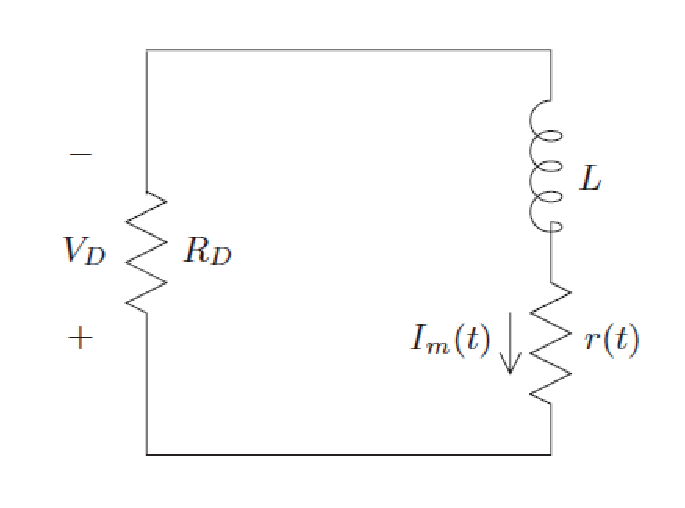
\includegraphics[scale=0.5]{chpt8/figs/fig8.3.eps}
\caption{电路模型:电感为$L$的超导磁体,有依赖于$T(t)$的正常区电阻$r(t)$,在放电模式下绝热加热。
	放电电阻$R_D$旁路磁体端子。$V_D\equiv R_d I_m(0)$是$t=0$时刻$R_D$上的放电电压}
\end{figure}

磁体电感$L$和放电电阻$R_D$可以分别由磁体初始存储磁能$E_m$和$R_D$上的初始放电电压$V_D$表示。即:
\begin{subequations}
	\begin{align}
	L&=\frac{2E_m}{I_{op}^{2}}\\
	R_D&=\frac{V_D}{I_{op}}
	\end{align}
\end{subequations}

联立8.16b,8.17a和8.17b,得到:
\begin{equation}% 8.18a
Z(T_f,T_i)=\left(\frac{A_m}{A_{cd}}\right)\frac{J_{m_o}^{2}E_m}{V_DI_{op}}
\end{equation}
该方程表明,$T_f$在大$J_{m_o}$和/或$E_m$以及小$V_D$和/或$I_{op}$的组合下较大。
我们可以考虑将比值$E_m/V_D I_{op}$作为有效放电时间,其中$V_D I_{op}$是有效放电功率。
由$J_{m_o}=I_{op}/A_m$,我们将8.18化简为:
\begin{align*}% 8.18b
Z(T_f,T_i)=\frac{J_{m_o}^{2}E_m}{A_{cd}V_D} \tag{8.18b}
\end{align*}

在放电模式下,对任意绕组温度极限$T_f$,存在一个最大的基底电流密度$J_{m_o}^D$:
\begin{equation}% 8.19
J_{m_o}^{D}=\frac{A_{cd}V_DZ(T_f,T_i)}{E_m}
\end{equation}

方程8.19给出了完全不同于6.22所给的低温稳定性判据的$J_{m_o}$判据。

\subsection{引线短接的磁体的绝热加热}
假设一个电感为$L$的磁体端子短接,在$t=0$时刻绕组中出现了一小块正常区域,如图8.4;
电流$I_m(t)$在电阻为$r(T)$的正常区基底金属流动。
\begin{figure}
	\centering
	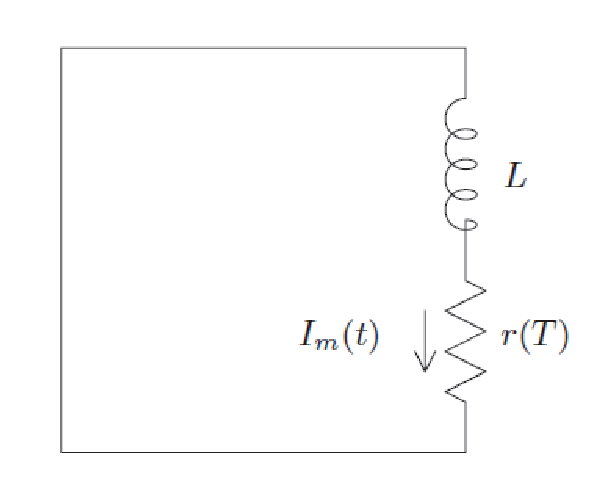
\includegraphics[scale=0.5]{chpt8/figs/fig8.4.eps}
	\caption{电路模型:电感为$L$的磁体端子短接,有依赖于温度的正常态区域电阻$r(T)$,绝热加热。
	正常态区域的电流为$I_m(t)$。}
\end{figure}

基底金属电流$I_m(t)$的控制方程为:
\begin{equation}% 8.20
L\frac{dI_m(t)}{dt}+r(T)I_m(t)=0
\end{equation}
温度依赖的$r(T)$显然随时间增加。有两个原因:1) 磁场能被转化为热能,使正常态区域温度升高;2)
正常态区域自身在绕组内扩散。
为了我们的分析,使用\textit{最简单}的假设:正常态区域电阻为常数,$r(T)=R_{nz}$:
\begin{equation}% 8.21
R_{nz}=\frac{\rho_m(T_f)\ell_{nz}}{4A_m}
\end{equation}
式中,$\rho_m(T_f)$是正常态最终温度下的基底电阻率;
$\ell_{nz}$是电流衰减到零时处于电阻态的总导体长度。
分母中的因子4来源于正常态区域温度$T_i$和$T_f$之间在空间(2)和时间(2)上的“平均”。
方程8.21同时假定了$\rho_m(T_f)\gg \rho_m(T_i)$,在一些特定的$T_i$和$T_f$组合下可能是不成立的,
但这个简化引入的不确定性相比8.21给出的基本假设引起的不确定性要小得多。
在$R_{nz}$时,$J_m(t)=I_m(t)/A_m$,由$J_m(t=0)=I_{op}/A_m=J_{m_o}$,得:
\begin{equation}% 8.22
J_m(t)=J_{m_o}e^{-t/(L/R_{nz})}
\end{equation}

在绝热加热时,我们得到:
\begin{subequations}% 8.23a,b,c
	\begin{align}
Z(T_f,T_i)&=\left(\frac{A_m}{A_{cd}}\right)\int_{0}^{\infty}J_{m_o}^{2}e^{-2t/(L/R_{nz})}dt\\
Z(T_f,T_i)&=\frac{1}{2}\left(\frac{A_m}{A_{cd}}\right)J_{m_o}^{2}\left(\frac{L}{R_{nz}}\right) \\
&=\frac{1}{2}\left(\frac{A_m}{A_{cd}}\right)J_{m_o}^{2}\tau_{dg}
\end{align}
\end{subequations}
式中,$\tau_{dg}=L/R_{nz}$是有效放电时间常数。
对一个参数为$a_1,\alpha$,总匝数为$N$的螺管线圈,驱动到正常态的总复合导体长度$\ell_{nz}$为:
\begin{equation}% 8.24
\ell_{nz}=f_r\pi a_1(\alpha+1)N
\end{equation}
式中,$f_r$是出于电阻态的绕组体积分数,与8.6同。
联立8.21和8.24,有:
\begin{equation}% 8.25
R_{nz}=f_r\frac{\rho_m(T_f)\pi a_1(\alpha+1)N}{4A_m}
\end{equation}

我们可以用$L$和其他磁体参数(方程3.81)表示$N$:
\begin{equation}% 8.26
N=\sqrt{\frac{L}{\mu_oa_1\ \mathcal{L}(\alpha,\beta)}}
\end{equation}

于是,$R_{nz}$可以写为:
\begin{equation}% 8.27
R_{nz}=f_r\frac{\pi(\alpha+1)\rho_m(T_f)}{4A_m}\sqrt{\frac{a_1L}{\mu_o\ \mathcal{L}(\alpha,\beta)}}
\end{equation}

这样,我们可以得到放电时间常数$\tau_{dg}$:
\begin{subequations}% 8.28a,b
	\begin{align}
\tau_{dg}&=\frac{L}{R_{nz}}=\frac{4A_m}{f_r\pi(\alpha+1)\rho_m(T_f)}\sqrt{\frac{\mu_o\ \mathcal{L}(\alpha,\beta)L}{a_1}}\\
\tau_{dg}&=\frac{4}{f_r\pi(\alpha+1)\rho_m(T_f)J_{m_o}}\sqrt{\frac{2\mu_o\ \mathcal{L}(\alpha,\beta)E_m}{a_1}}
\end{align}
\end{subequations}
式中,$J_{m_o}=I_{op}/A_m, L=2E_m/I_{op}^2$,其中$E_m$是磁体的初始磁场能储量。

联立8.23c和8.28b,有:
\begin{equation}% 8.29
\rho_m(T_f)Z(T_f,T_i)=\left(\frac{A_m}{A_{cd}}\right)\frac{2J_{m_o}}{f_r\pi(\alpha+1)}\sqrt{\frac{2\mu_o\ \mathcal{L}(\alpha,\beta)E_m}{a_1}}
\end{equation}

方程8.29中可以解出$T$。
如前面8.1.2所提及的,$T_f$严重依赖于$f_r$。对于8.1.2中的实例,为了在$B_o\ge 5$ T时确保$T_f$低于200 K,$f_r$至少$\sim 0.1$。
这个条件对具有小正常区传播(NZP)速度的HTS是很难满足的,8.4会继续讨论。

尽管$f_r$是未知的,但对一个给定的$T_f$和$T_i$组合,存在一个最大基底电流密度$J_{m_o}^{sh}$限制了短接磁体的过热:
\begin{subequations}% 8.30a,b
	\begin{align}
J_{m_o}^{sh}=\frac{1}{2}\left(\frac{A_{cd}}{A_m}\right)f_r\pi(\alpha+1)\rho_m(T_f)Z(T_f,T_i)\sqrt{\frac{a_1}{2\mu_o\ \mathcal{L}(\alpha,\beta)E_m}}\\
J_{m_o}^{sh}(T_f,T_i)=\frac{1}{2}\left(\frac{A_{cd}}{A_m}\right)\frac{f_r\pi(\alpha+1)\rho_m(T_f)Z(T_f,T_i)}{\mu_o\ \mathcal{L}(\alpha,\beta)NI_{op}}
\end{align}
\end{subequations}
b式是在a式中代入$E_m=\mu_o a_1\mathcal{L}(\alpha,\beta)N^2 I_{op}^2/2$得到的。
如我们所料,$J_{m_o}^{sh}$在大$f_r$和$T_f$以及小$E_m$组合下为增函数。
8.30b表明,大安匝数的螺管线圈必须在小$J_{m_o}^{sh}$下运行。


\subsection{恒定电压模式下的绝热加热}
最后,考虑一个超导磁体,整个绕组全部为电阻性,导体总长度为$\ell_{cd}$,电阻为$R_m(T)$,连接于恒定电压源,如图8.5所示。
这里,整个绕组的温度为$T(t)$。
考虑$R_m(T)=\rho_m(T)\ell_{cd}/A_m$,功率密度方程类似于8.9a:
\begin{subequations}% 8.31a,b
	\begin{align}
A_{cd}\ell_{cd}C_{cd}(T)\frac{dT}{dt}&=\frac{V_{op}^{2}}{R_n(T)}=\frac{V_{op}^{2}A_m}{\rho_m(T)\ell_{cd}}
C_m(T)\frac{dT}{dt}\\
&\simeq\left(\frac{A_m}{A_{cd}}\right)\frac{V_{op}^{2}}{\rho_m(T)\ell_{cd}^{2}}\\
\int_{T_i}^{T_f}C_m(T)\rho_m(T)dT&=\left(\frac{A_m}{A_{cd}}\right)\frac{V_{op}^{2}}{\ell_{cd}^{2}}\tau_{ah}
\end{align}
\end{subequations}
式中,$\tau_{ah}$是在恒定电压模式下的加热时间。
根据$Z(T_f,T_i)$,我们可以定义函数$Y(T_f,T_i)$。类似于8.10b,可以针对合金基底金属作简化。类似于$Z(T_f,T_i)$,$Y(T_f,T_i)$
也可以写成两个单一温度的函数。
\begin{subequations}% 8.32a,b,c
	\begin{align}
Y(T_f,T_i)&\equiv\int_{T_i}^{T_f}C_m(T)\rho_m(T)dT\\
Y(T_f,T_i)&\simeq\tilde{\rho}_m[H_m(T_f)-H_m(T_i)]\\
Y(T_f,T_i)&=Y(T_f)-Y(T_i)
\end{align}
\end{subequations}

图8.6给出了$Y(T,0)$图,该图中的金属和图8.2中的$Z(T,0)$所对应的相同。
金属的纯度,通常在$\sim$50 K之下对$\rho_m$影响很大。
于是,纯度对$Z(T,0)$想想很大,而对$T>\sim$100 K时的$Y(T,0)$影响很小。

类似于8.9c,我们从8.31b可以导出:
\begin{equation}% 8.33
Y(T_f,T_i)=\left(\frac{A_m}{A_{cd}}\right)\frac{V_{op}^{2}\tau_{ah}}{\ell_{cd}^{2}}
\end{equation}
\begin{figure}
	\centering
	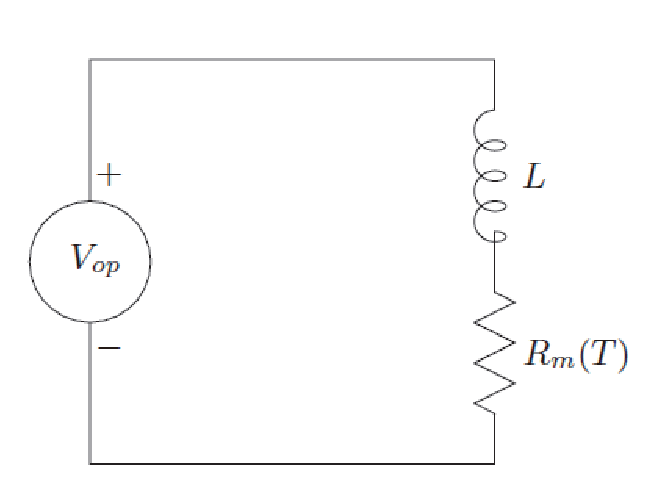
\includegraphics[scale=0.5]{chpt8/figs/fig8.5.eps}
	\caption{电路模型:电感为$L$的超导磁体,全部绕组处于正常态,电阻为$R_m(T)$,在恒压源加热模式。}
\end{figure}

注意到螺管线圈在$f_r=1$的$\ell_{cd}$已由8.24给出,使用8.26,我们得到:
\begin{equation}% 8.34
\ell_{cd}=\pi(\alpha+1)\sqrt{\frac{a_1L}{\mu_o\ \mathcal{L}(\alpha,\beta)}}
\end{equation}

将8.34中的$\ell_{cd}$代入8.33,有:
\begin{equation}% 8.35
Y(T_f,T_i)=\left(\frac{A_m}{A_{cd}}\right)\frac{\mu_o\ \mathcal{L}(\alpha,\beta)V_{op}^{2}\tau_{ah}}{\pi^2(\alpha+1)^2a_1L}
\end{equation}

对任意$T_f$和$T_i$组合,在恒压加热模式下,存在一个加热时间极限$\tau_{ah}^v$:
\begin{equation}% 8.36
\tau_{ah}^{\upsilon}=\left(\frac{A_{cd}}{A_m}\right)\frac{\pi^2(\alpha+1)^2a_1L}{\mu_o\ \mathcal{L}(\alpha,\beta)}\left[\frac{Y(T_f,T_i)}{V_{op}^{2}}\right]
\end{equation}

因为$\rho_m(T)$随温度$T$增加,$Y(T,0)$在$T$超过300 K之后继续增加。
因为超导磁体处于正常态的总电阻$R_m(T)$正比于$\rho_m(T)\ell_{cd}$,
通过磁体的加热电流由$V_{op}/R_m(T)$给出,它随$T$增加而减小。
这意味着$\tau_{ah}^v$比$T_f$增加的更快;也即在恒压加热模式下,比在恒流模式下更不容易热失控。
因此,就加热超导磁体而言,恒压模式要比恒流模式更安全。本问题将在问题8.1中进一步研究。

\begin{figure}
	\centering
	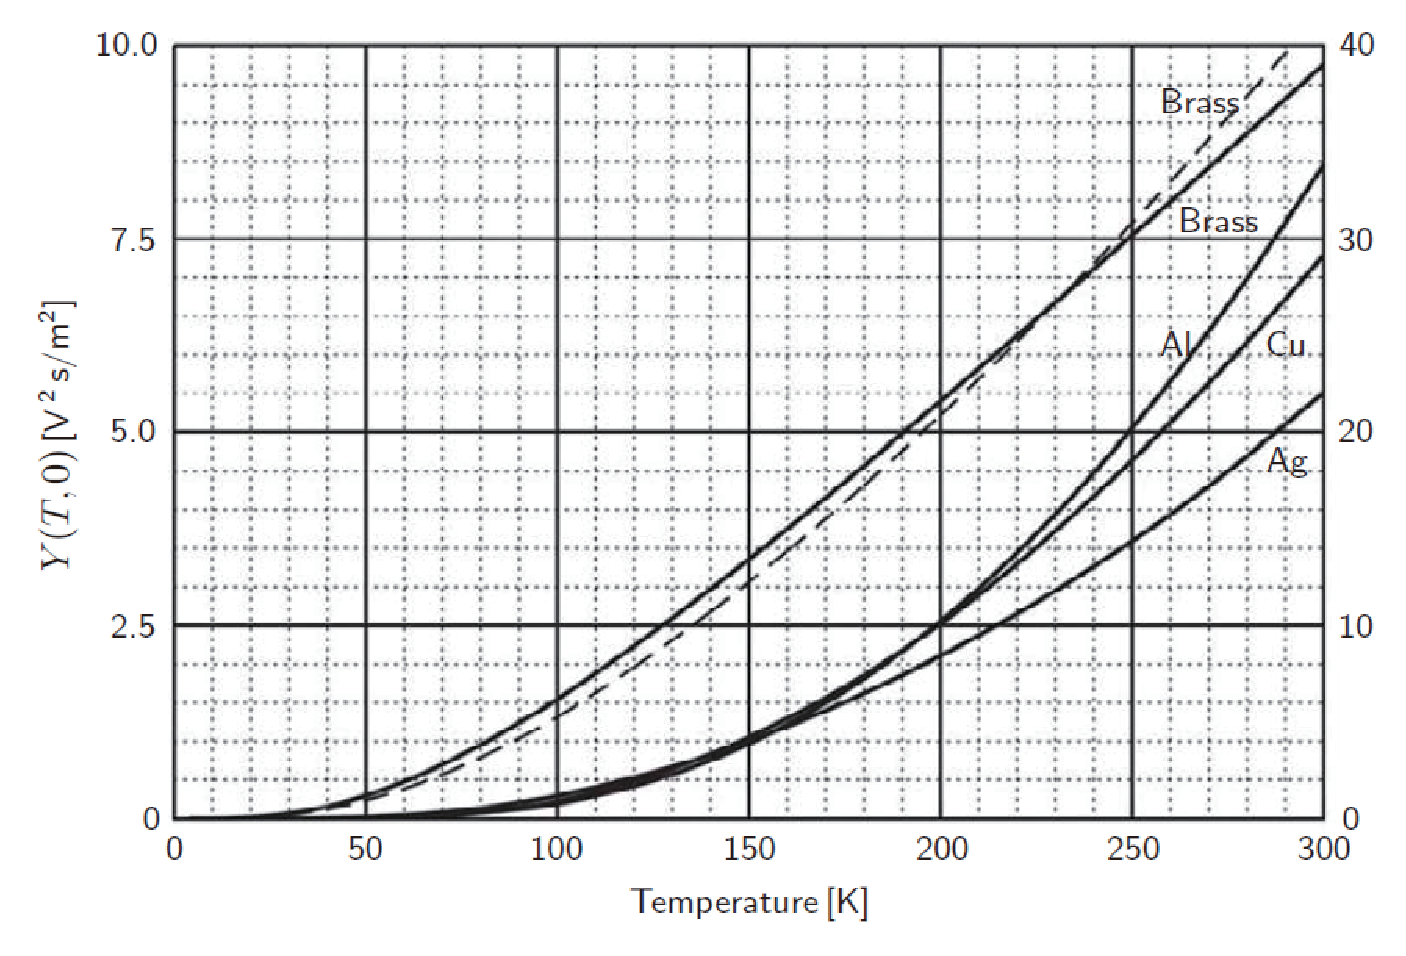
\includegraphics[scale=0.5]{chpt8/figs/fig8.6.eps}
	\caption{$Y(T,0)$图。左侧纵轴是Ag、Cu、Al的刻度,右侧纵轴是黄铜的刻度。
	在温度超过约100 K后,$Y(T,0)$几乎与Ag和Cu的纯度无关。}
\end{figure}



\section{高电压}
大多数超导磁体的一个吸引人的特征是励磁所需的“低”电压,即$\sim$10 V。对于产生相同场强的普通金属磁体该值$>100$ V。
磁体运行包括三个时间区间:1)充电励磁; 2)恒定磁场静态运行; 3)放电去磁。 
不幸的是,这种低电压充足性通常仅在前两个时间区间可以保证;
区间3可能遇到非常高的电压,特别是它处于故障模式的时候。
 当然,由于磁体失超,在区间1和区间2期间可能会突然进入区间3。
 由于超导磁体是电感器,其端电压包含一个电感分量,由下式给出:
 \begin{align}
V=L\frac{dI}{dt}
 \end{align}
注意到$L=2E_m/I_o^2$,其中$I_o$是区间3开始时的磁体电流。
因为在这个区间,磁体电流下降$\Delta I$通常等于$I_o$,我们可以将8.37改写为:
\begin{align*}
V=\frac{2E_m}{I_{o}^{2}}\left(\frac{\Delta I}{\Delta t}\right)\approx\frac{2E_m}{I_o\Delta t}\tag{8.37b}
\end{align*}

保护主要在那些$E_m$超过$\sim$ 100 kJ的磁体才非常关键;
储能量小于这个级别的磁体是可以补救的,或者至少不会引起严重的困难。
如果我们设定实际超导磁体的危险电压等级是1 kV,那么根据8.37b,
在$E_m=100$ kJ时,任意小于200 As的$I_o\Delta t$组合值都会产生高于1 kV
的电压,磁体中的能量将足以引起严重破坏。
一个实例:运行于$I_o=1$ kA的100 kJ磁体,如果电流在$\sim$200 ms级别放电。
随着储能量的增加,问题越来越严重[8.17]。

根据8.37b,我们还可以看到,电流引线必须承受较高的放电电压。
Anishchenko、Heller等[8.18]和Gerhold[8.19]已开发出可以承受高压的电流引线。

\subsection{电弧环境}
超导绕组可能工作于一个设计者可以选择的环境中,比如1) 真空 vs. 非真空;2) 液体 vs. 气体;和/或 3) 氦 vs. 氮。
在防止电弧方面,除了在Paschen压力附近,真空要优于非真空;液体优于气体;氮优于氦.
不过,放电可能会破坏设计者的环境选择。
故障引起的绕组加热会破坏设计条件:1)它可能加快系统排气,使系统维持高真空变得困难;或者2)它可能将局部的环境从液体变为气体。

自1970年代初,人们开始归集制冷工质的绝缘击穿数据[8.20,8.21]。
Gerhold给出了氮和氦的击穿数据[8.22]。
在超导磁体中,存在很多影响电弧的设计项目,尚无普适的明确数据。
Schultz简明的探讨了这个大问题,给出了不少图表和数据[1.28,8.11]。

表8.4.。。。。。。。。。。。。。。。

\subsection{Paschen电压试验}
表8.4给出了\textit{室温}气体的最小电弧放电电压$V_{mn}$以及对应的$Pd$数据。
$P$是气体压力,$d$是施加电压$V_{mn}$的电极距离。
注意到双原子分子的$V_{mn}$要比惰性气体的搞。

Paschen电压试验是放电电压超过1 kV的超导磁体的例行试验。
低温容器试验时,将电流引线和测试电缆连接于高压,将低温容器抽空至某压力(如$P\sim 10^{-3}$ torr)之下。
如果在电压升高至$V_{mn}$期间没有泄漏电流,则在下一个压力水平下(从$P\sim 10^{-2}$ torr到大气压)重复上述试验。
系统在进行更复杂的高压测试前,必须通过如上简单的试验。

\subsection{失超磁体内的电压峰值}
使用一个简单的模型,引入额外的简化假设,我们研究失超超导磁体在其端子短接时的内部电压峰值[1.27;8.25]。
在以下两种超导磁体模式下,端子短接工况在一个很短的时间内很可能出现:
1) 在区间1,当磁体连接于恒压电流源,磁体电流增至进入它的区间2;
2) 当区间2的磁体被持续模式开关旁路。
任一模式下,当故障迫使(主动保护)或自动(被动保护)地令超导磁体进入区域3,端子不能在被视为短接。
不过,在这个时候,特别是当磁体是主动保护的时候,因为转移的延迟,损坏可能已经发生。

\textbf{内部电压分布}

在一个内部正常区扩散的旁路磁体中,内部电压的分布与绕组内的正常区分布有关。
图8.7给出了磁体内的电压分布,其中绕组从接地的端子绕向另一个接地的端子。
单位导体长度的电感假定为常数。
在8.7a中,10\%($f_r=0.1$)的绕组从一个端子开始,已经进入电阻态;
在8.7b中是20\%;在8.7c中是50\%;在8.7d中是100\%。

\begin{figure}
	\centering
	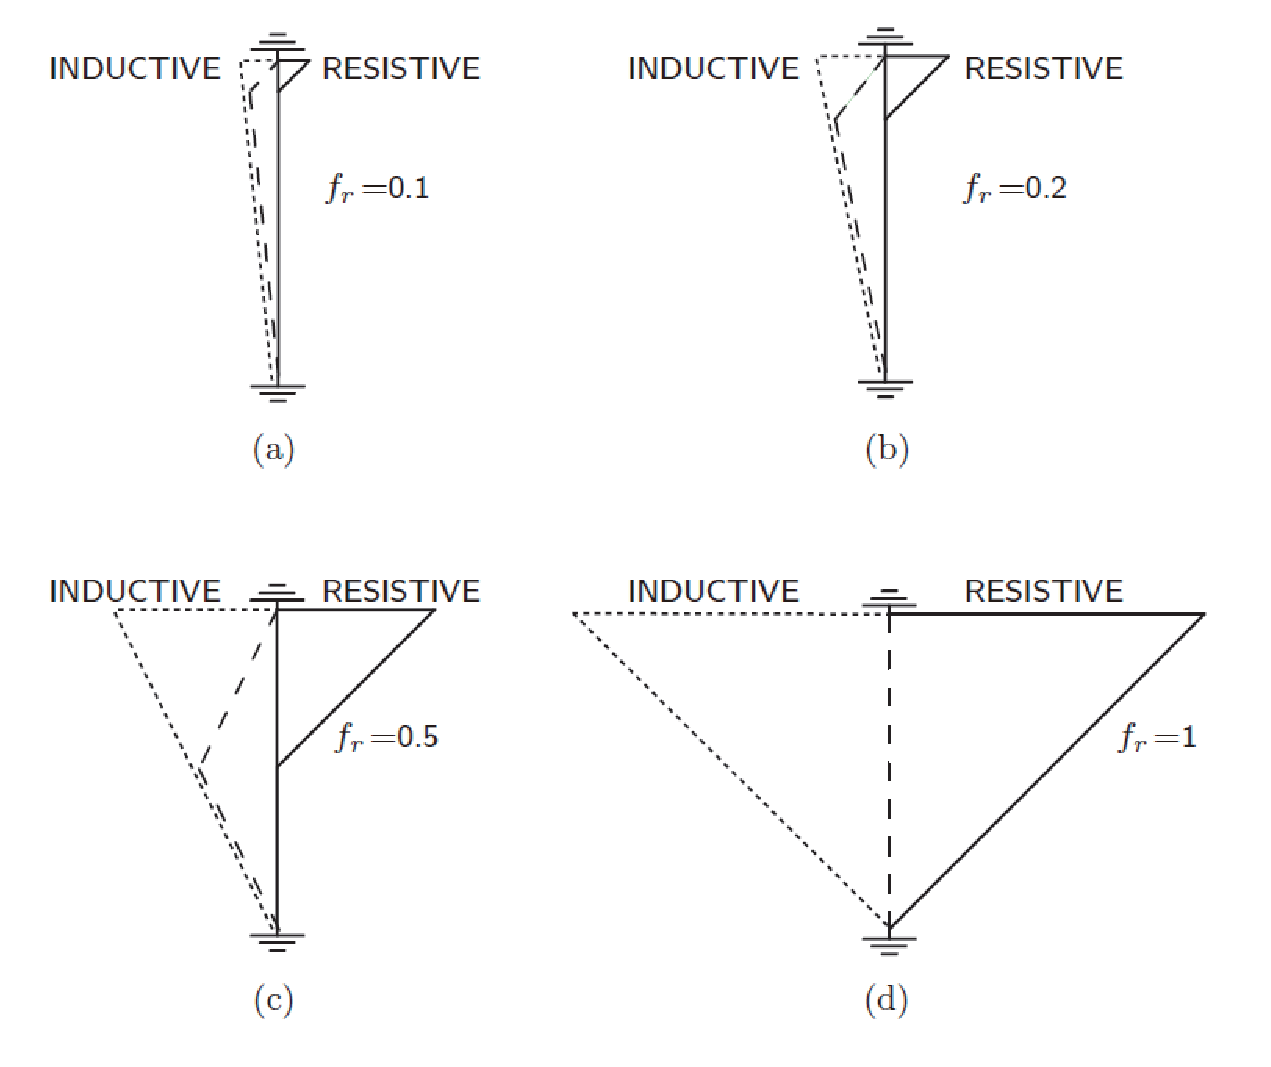
\includegraphics[scale=0.5]{chpt8/figs/fig8.7.eps}
	\caption{电压分布。}
\end{figure}

在图8.7的每一组电压分布中,实线表示阻性电压;短虚线表示感性电压;长虚线表示作为电阻性和点感性电压之和的总内部电压。
每一个图中,磁体电流保持恒定为$I_{op}$。
实际中,电流似乎随时间减小的;这个减小的效应在后面将会考虑。

最高阻性电压$[V_r]_{mx}$发生在磁体的一个端子上。因为端子是接地的,它恰好与同等复制的感性电压$[V_r]_{mx}=R_{nx}I_{op}$匹配,
其中$R_{nx}$是总的正常态电阻,如方程8.25所给。

从图8.7中我们得到最大内部电压为:
\begin{equation}% 8.38
[V_{in}]_{mx}=f_r(1-f_r)R_{nz}I_{op}
\end{equation}
其中,$f_r$如方程8.6已指出的,是被驱至电阻态的绕组体积分数。
注意到磁体电流维持$I_{op}$。
方程8.38表明在$f_r\rightarrow 0$或$f_r\rightarrow 1$时有$[V_{in}]_{mx}\rightarrow 0$。
方程还表明$[V_{in}]_{mx}$的峰值出现在$f_r=0.5$。

联立8.25和8.38,有:
\begin{equation}% 8.39
[V_{in}]_{mx}=f_r(1-f_r)\frac{\pi(\alpha+1)\rho_m(T_f)a_1}{4A_m}NI_{op}
\end{equation}

\textbf{基底电流密度的电压判据}

最大内部电压出现的条件为:正常区扩散到占绕组的$50\%$而电流仍维持$I_{op}$;或初始时绕组即有50\%被驱至正常态。

我们可以得到限制带旁路螺管磁体内部感应电压不超过击穿值$V_{bk}$的基底电流密度$J_{m_o}^V$的表达式:
\begin{equation}% 8.40a
J_{m_o}^{V}=\frac{2}{f_r(1-f_r)}\left[\frac{F(\alpha,\beta)}{\pi(\alpha^2-1)\beta}\right]\left[\frac{\mu_oV_{bk}I_{op}}{a_{1}^{2}\rho_m(T_f)B_o}\right]
\end{equation}
类似的,我们可以得到一个直接看出与$E_m$依赖关系的表达式:
\begin{align*}% 8.40b
J_{m_o}^{V}=\frac{2}{f_r(1-f_r)}\left[\frac{\sqrt{\ \mathcal{L}(\alpha,\beta)}}{\pi(\alpha+1)}\right]\left[\frac{V_{bk}I_{op}}{\rho_m(T_f)}\sqrt{\frac{2\mu_o}{a_1E_m}}\right] \tag{8.40b}
\end{align*}

可以看到,$J_{m_o}^V$随$V_{bk}$和$I_{op}$的乘积增长。
这里最重要的是,$J_{m_o}^V$随正常态金属的电导率增大而提高。
此外,一个较大的$V_{bk}$意味着较大的$J_{m_o}^V$,但是$I_{op}$下的绕组的电流密度$\lambda J_{op}$(6.3.3)
因为需要更多绝缘会很小。

\section{正常区传播(NZP)}
为了保护,多数“实际”大小的HTS磁体都必须依赖于一类或另一类主动技术,其中的一些将在后文讨论。
不过,对任何主动保护技术,因为在非恢复正常区的检测和电流退降之间存在不可避免的延迟,所以令磁体的正常区域传播(NZP)
速度“加快”,进而扩大其$f_r$(它限制$e_{mr}$(方程8.7),加强$J_{m_o}^{sh}$(方程8.30)和$J_{m_o}^V$(方程8.40))就很重要了。
一个具有快NZP速度(三个方向)的磁体可以成为“自保护”的;
自保护磁体的更多细节后文将讨论。
因为NZP速度在HTS绕组中通常比在LTS绕组中慢很多,故“自保护”HTS磁体几乎不可能实现:
\textit{所有}的HTS磁体都需要主动保护。

\subsection{轴向NZP速度}
自1960年代以来,LTS和HTS测试样品、模型绕组和磁体在绝热、准绝热、冷却条件下的长度方向
(沿着导体轴向)的NZP速度$U_\ell$得到了全面的研究[8.1, 8.2, 8.25–8.75]。
它是高性能(绝热)磁体保护的重要参数之一。
在那些绝热或准绝热的绕组中,NZP不仅限于导体轴向,而是三维扩散的:$U_t\propto U_\ell$,
其中$U_t$是“横向”传播速度。

\subsubsection*{绝热条件下的NZP}
图8.8给出了绝热条件下载流为$I$的导体示意图,正常-超导边界在$x=0$处,边界以恒定速度$U_\ell$沿$+x$方向移动。
正常态超导体的功率密度方程由不含扰动和冷却项的方程6.1的一维($x$)形式给出:
\begin{equation}% 8.41a
C_n(T)\frac{\partial T_n}{\partial t}=\frac{\partial}{\partial x}\left[k_n(T)\frac{\partial T_n}{\partial x}\right]+\rho_n(T)J^2
\end{equation}
其中,$C_n(T),k_n(T)$和$\rho_n(T)$分别是正常态超导体的热容、热导率和电阻率。

\begin{figure}
	\centering
	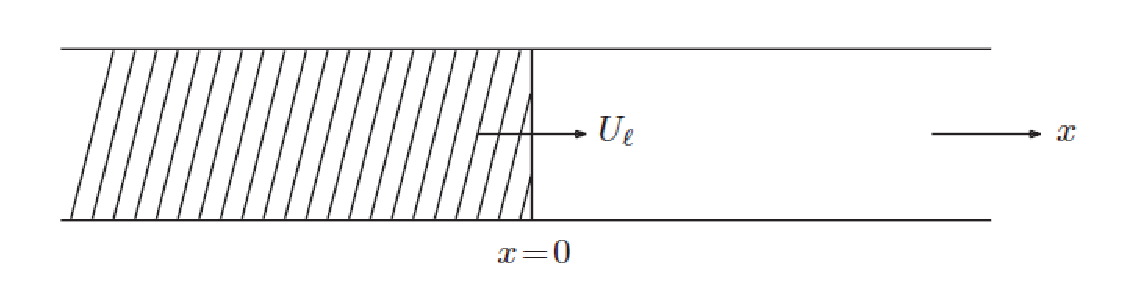
\includegraphics[scale=0.6]{chpt8/figs/fig8.8.eps}
	\caption{一维正常-超导边界($x=0$)以恒定速度$U_\ell$沿长度方向(轴向)移动。阴影部分($x<0$)
		为正常态区域,右侧为超导区域。}
\end{figure}

类似的,超导区域在绝热条件下的$x$方向的功率密度方程为:
\begin{align*}% 8.41b
C_s(T)\frac{\partial T_s}{\partial t}=\frac{\partial}{\partial x}\left[k_s(T)\frac{\partial T_s}{\partial x}\right] \tag{8.41b}
\end{align*}
其中,$C_s(T),k_s(T)$是超导态的热容和热导率。
当正常-超导边界在$+x$方向以恒定速度$U_\ell$移动时,我们可以将$x$坐标变换为$z$坐标:$z=x-U_\ell t$。
$\partial T_n/\partial t$可以写为:
\begin{equation}% 8.42
\frac{\partial T_n}{\partial t}=\frac{\partial T}{\partial z}\frac{\partial z}{\partial t}=-U_\ell\frac{dT}{dz}
\end{equation}

于是,我们可以吧8.41写成:
\begin{subequations}
	\begin{align}
-C_n(T)U_\ell\frac{dT_n}{dz}=&\frac{d}{dz}\left[k_n(T)\frac{dT_n}{dz}\right]+\rho_n(T)J^2\\
-C_s(T)U_\ell\frac{dT_s}{dz}=&\frac{d}{dz}\left[k_s(T)\frac{dT_s}{dz}\right]
	\end{align}
\end{subequations}
整理8.43a和8.43b,我们得到超导体分别在超导区($z>0$)和正常区($z<0$)的能量密度方程:
\begin{subequations}
	\begin{align}
&(z<0)\quad      \frac{d}{dz}\left[k_n(T)\frac{dT_n}{dz}\right]+C_n(T)U_\ell\frac{dT_n}{dz}+\rho_n(T)J^2&=0\\
&(z>0)\quad      \frac{d}{dz}\left[k_s(T)\frac{dT_s}{dz}\right]+C_s(T)U_\ell\frac{dT_s}{dz}&=0
	\end{align}
\end{subequations}
令$C_n(T),k_n(T), C_s(T)$和$k_s(T)$均为常数,分别记为$C_n,k_n, C_s$和$k_s$。假设$d^2 T_n/dz^2\simeq 0$,
我们可以重写8.44:
\begin{subequations}
	\begin{align}
	&(z<0)\quad     C_nU_\ell\frac{dT_n}{dz}+\rho_nJ^2&=0\\
&	(z>0)\quad     k_s\frac{d^2T_s}{dz^2}+C_sU_\ell\frac{dT_s}{dz}&=0
	\end{align}
\end{subequations}

从8.45b中可以直接解出$T_s(z)$:
\begin{equation}% 8.46a
T_s(z)=Ae^{-cz}+T_{op}
\end{equation}
式中,$T_{op}$是远离$z=0$($z\gg 0$)处的运行温度,
$c=C_s U_\ell/k_s$。
我们还知道$z=0$时由$T_s=T_t$,其中$T_t$是载流为$I$的超导体的转变温度。于是:
\begin{align*}% 8.46b
T_s(z)=(T_t-T_{op})\exp\left(-\frac{C_sU_\ell}{k_s}z\right)+T_{op} \tag{8.46b}
\end{align*}

另一个边界条件是各区域的$k(dT/dz)$应该在$z=0$处相等---
热流必须在边界上连续:
\begin{equation}% 8.47a
k_n\frac{dT_n}{dz}\mid_0=k_s\frac{dT_s}{dz}\mid_0
\end{equation}
联立8.45a,8.46b和8.47a,有:
\begin{align*}% 8.47b
-\frac{k_n\rho_nJ^2}{C_nU_\ell}=-C_sU_\ell(T_t-T_{op}) \tag{8.47b}
\end{align*}
在8.47b中解出$U_\ell$,有:
\begin{equation}% 8.48
U_\ell=J\sqrt{\frac{\rho_nk_n}{C_nC_s(T_t-T_{op})}}
\end{equation}

方程8.48中重要的几点包括$U_\ell$直接正比于电流密度$J$,而反比于两个区域热容的几何平均$\sqrt{C_n C_s}$。
8.48给出的$U_\ell$对绝热条件下的裸超导体有效。
由于材料物性是温度依赖的,使用$U_\ell$的精确表达式没什么必要。不过出于完整性,我们给出下面的精确表达式[8.47]:
\begin{equation}% 8.49
U_\ell=J\sqrt{\frac{\rho_n(T_t)k_n(T_t)}{\left[C_n(T_t)-\frac{1}{k_n(T_t)}\frac{dk_n}{dT}\mid_{T_t}\int_{T_{op}}^{T_t}C_s(T)dT\right]\int_{T_{op}}^{T_t}C_s(T)dT}}
\end{equation}

方程8.49给出的$U_\ell$值与YBCO带材短样在45-77 K的实测值吻合很好[8.66]。

取材料物性为常数,我们发现8.49退化为8.48。
在$C_n=C_s=C_o$时,方程8.48可以写为:
\begin{equation}% 8.50a
U_\ell=\frac{J}{C_o}\sqrt{\frac{\rho_nk_n}{(T_t-T_{op})}}
\end{equation}
在$(T_t-T_{op})/T_{op}\ll 1$时(一个通常可用于LTS而不能用于HTS的条件),我们可以修正8.50a,让它包含
温度依赖的$C_o,\rho_n$和$k_n$:
\begin{align*}% 8.50b
U_\ell=\frac{J}{C_o(\tilde{T})}\sqrt{\frac{\rho_n(\tilde{T})k_n(\tilde{T})}{(T_t-T_{op})}} \tag{8.50b}
\end{align*}
式中,$\tilde{T}=(T_t+T_{op})/2$。
方程8.48到8.50对没有基底金属的超导体有效;
实际中,磁体级导体都是复合的,我们可以用基底金属材料的物性近似上述材料属性。

\subsubsection*{复合超导体}
对于有截面为$A_m$的基底金属的复合导体,在$(T_t-T_{op})/T_{op}\ll 1$时(同样,只适用于LTS),
引入温度依赖的参数,利用$\tilde{T}=(T_t+T_{op})/2$,将8.50b推广为:
\begin{equation}% 8.51a
U_\ell=\frac{J_m}{C_{cd}}(\tilde{T})\sqrt{\frac{\rho_m(\tilde{T})k_m(\tilde{T})}{T_t-T_{op}}}
\end{equation}
式中,$C_{cd}(\tilde{T})$是导体在$T_{op}$和$T_t$区间的单位体积平均热容,
$J_m$是基底金属截面上的电流密度。
因为$\rho_m$(基底金属电阻率)远小于$\rho_n$,
$k_m$(基底金属热导率)远大于$k_n$,
8.51a中使用$k_m(\tilde{T})$和$\rho_m(\tilde{T})$是非常合适的。
方程8.51a中,Joshi建议转变温度$T_t\equiv (T_{cs}+T_{c})/2$[8.45],或简单的$T_t= (T_{cs}$。
试验数据很难验证这个微小的差异。
基于和方程8.9b相同的近似方法,我们使用$C_{cd}(\tilde{T})\simeq C_m(\tilde{T})$,有:
\begin{align*}% 8.51b
U_\ell\simeq\frac{J_m}{C_m}(\tilde{T})\sqrt{\frac{\rho_m(\tilde{T})k_m(\tilde{T})}{T_t-T_{op}}} \tag{8.51b}
\end{align*}

方程8.48-8.51的一般适用性已被大量LTS和最近的HTS试验证实。

\subsubsection*{长度方向NZP速度的实验确定}
确定$U_\ell$的实验基本装置很简单。
一般的,如图8.9所示,在一个长直样品上,测量很多短距离(10-20 cm)的局部电压信号;
在一些实验中,还监测了局部的温度。
如果测试样品处于磁体室温孔中,样品更倾向于环形或螺旋形而非平直的。
测试样品载流$I$时,由加热器等制造一个局部失超区域。
其过程通过电压信号$V_1,V_2,V_3$以及$V_\Sigma =V_1+V_2+V_3$监测;
明显,$U_\ell$可以从相邻电压(和/或温度)信号间距以及时间获得。
图8.9b给出了一段10 cm长Nb3Sn带的$V_1,V_2,V_3$以及$V_\Sigma =V_1+V_2+V_3$的记录波形[8.55]。

\begin{figure}
	\centering
	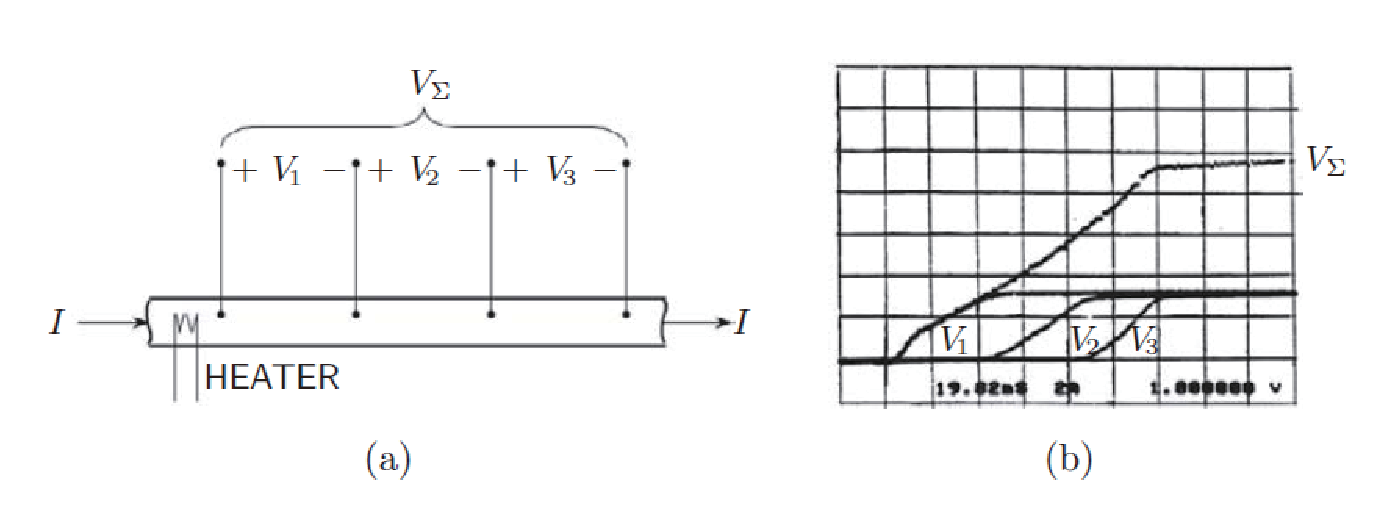
\includegraphics[scale=0.5]{chpt8/figs/fig8.9.eps}
	\caption{(a) 测量长度方向NZP速度的实验装置示意图;
		(b) NZP时间下的电压记录波形图。}
\end{figure}

使用类似于LTS测试所用的实验技术,在20实际初测量了上面描述的一个样品。
这里,不涉及实验设置的细节,我们仅在图8.10给出YBCO带材NZP速度测量的电压和温度的共四组曲线:
a),b)和c)是测试样品长度分别为20 cm[8.65],15 cm[8.70]和18 cm[8.74]情况下的$V(t)$曲线。
在20 cm场YBCO带材中,初始温度为50 K的样品的局部正常区域的产生依赖于在20 cm长度上的临界电流的非均匀分布。
72 A的过流脉冲(图8.10a和8.10d)触发了区域5的失超(相应的,$V_5$和$T_5$),导致恒定电流为30 A的NZP(图8.10a);
a)中的$V(t)$的时间刻度和d)中$T(t)$的时间刻度是一致的。
b)中的$V(t)$曲线是15 cm长带材在60 K的;c)中的是在70 K的。
测到的NZP速度在2-10 mm/s之间,总结如表8.5。

\begin{figure}
	\centering
	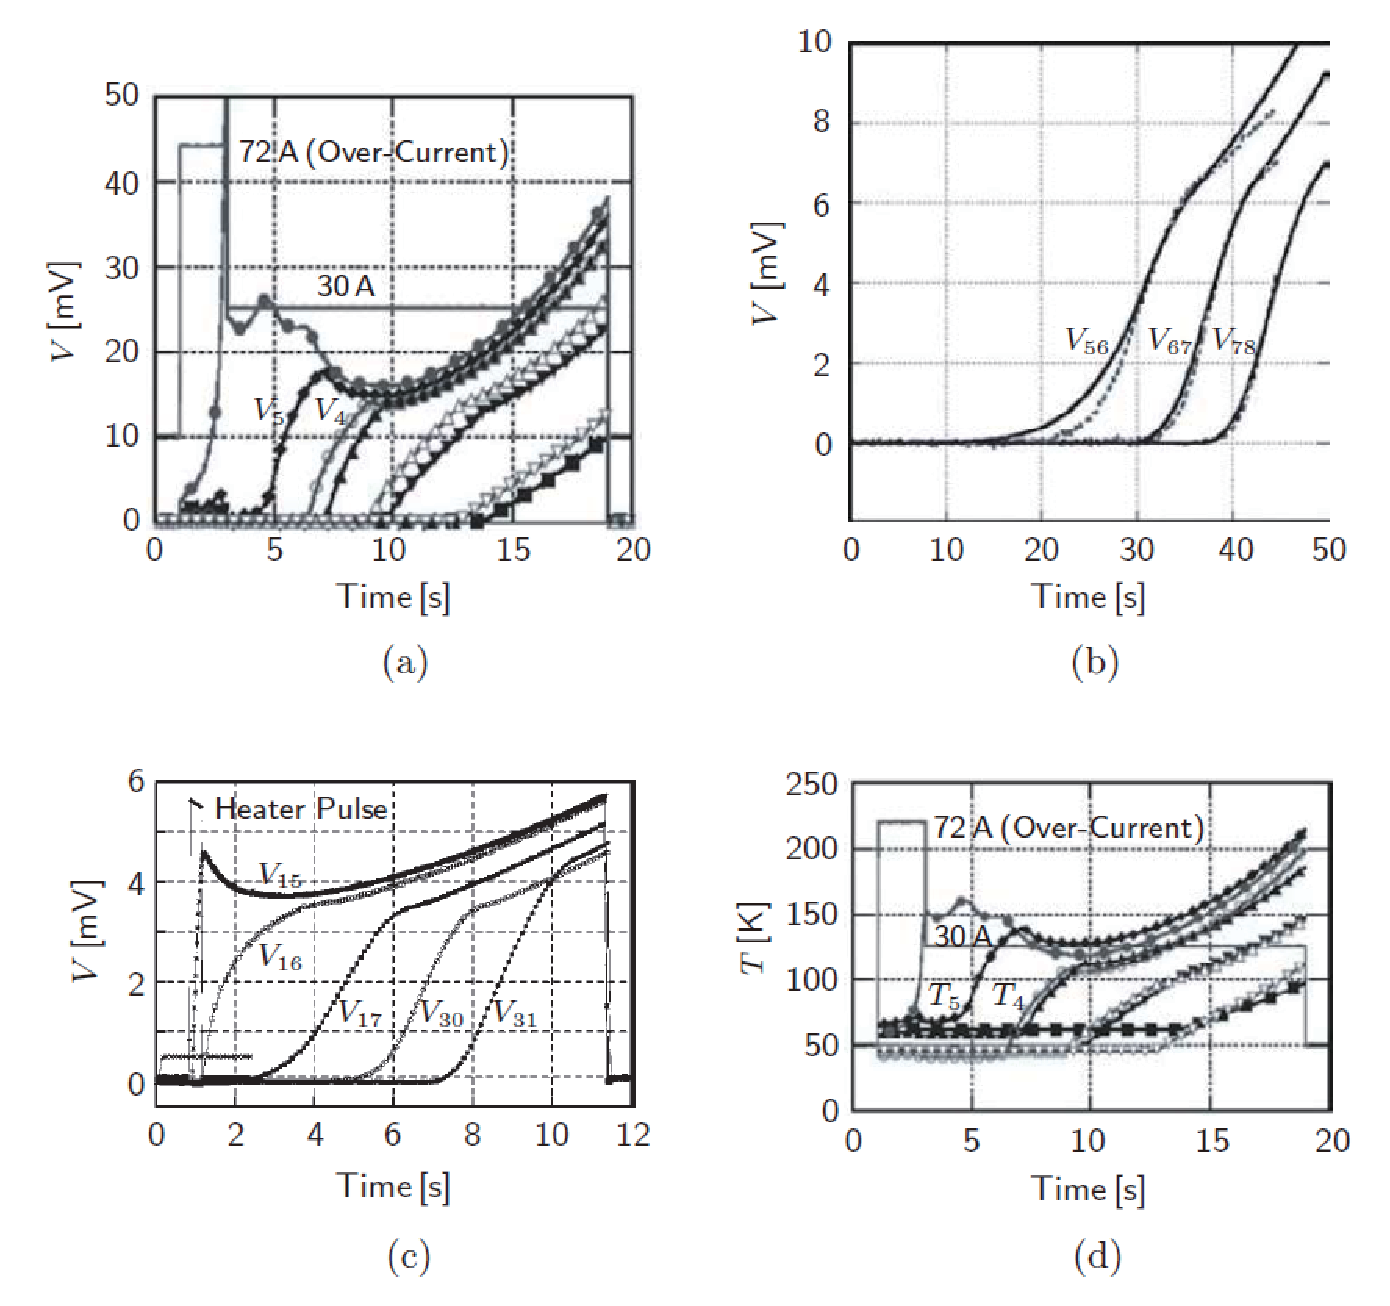
\includegraphics[scale=0.5]{chpt8/figs/fig8.10.eps}
	\caption{YBCO测试样品在长度方向的NZP信号。}
\end{figure}

表8.5.。。。。。。。。。。。。。。。。

表8.5列出了LTS和HTS的$U_\ell$测量值。
尽管由液氦冷却,Nb-Zr单丝的$U_\ell\propto J$,因为没有基底金属(Stekly之前时代的超导体),
正常态焦耳热完全超过了冷量。
一般的,这些数据表明HTS(Bi2223-Ag;YBCO)的NZP速度比LTS的小2-4个数量级。
NbTi的“恢复”[8.36]将在8.4.2讨论。
铁基底的MgB2[8.70],NZP速度和LTS的具有可比性,主要因为没有高导电基底金属。
这里,在总导体电流密度$J_{cd}$为$26\ \mathrm{ A/mm^2}$或更低时,
不会发生NZP:正常态超导体不产生足够的焦耳热,主要原因是其指数很低($n\simeq 15$)。
类似的非NZP行为在Bi2223-Ag[8.55]带和YBCO带[8.64,8.69,8.73]中都观察到了。

\subsection{“制冷”条件下的NZP}
尽管在冷却磁体中的NZP保护不及绝热磁体中那么重要,
但在有冷却条件下的NZP也获得了广泛的研究。
如表8.5中给出NbTi复合导体中观察到的,实际上存在一个“恢复”电流,低于
这个电流,正常态会缩小而不是扩大。

\subsection{横向(匝间)速度}
现在我们关注主要针对超导带材的横向(匝间)NZP速度$U_t$。
$\mathrm{Nb_3Sn}$带材曾一度很流行,但现在已不再用。
现在最广泛使用的复合超导体带材是HTS的Bi2223-Ag和YBCO,两者都可绕成饼式线圈。
此类HTS磁体的绕组尽管由制冷工质或制冷机冷却,但本质上是绝热的。
$U_\ell$的绝热分析可以用于导出$U_t$[8.57]:
\begin{equation}% 8.52
U_t=U_\ell\sqrt{\frac{1}{2}\left(\frac{\delta_{cd}}{\delta_i}\right)\left[\frac{k_i(\tilde{T})}{k_m(\tilde{T})}\right]}
\end{equation}
式中,$k_i(\tilde{T})$是相邻厚度为$\delta_{cd}$超导带之间的厚度为$\delta_i$的绝缘层的温度平均热导率。
方程8.52中,一般$\delta_{cd}>\delta_i$,倍数通常在3-10之间,但是$k_m\gg k_i$的倍数在1000或更大,
甚至在77 K时也是如此;所以,$U_t$至少比$U_\ell$小1到2个数量级。
Bi2223-Ag和YBCO模型线圈的测试实际上已经表明$U_t$至少比$U_\ell$小一个数量级。
因为有高导电基底的HTS的$U_\ell$本身仅为1-10 mm/s,$U_t$则更小。
如下面将讨论的,在2D和3D绕组中,接触热阻能进一步降低有效$U_t$。

\subsubsection*{接触热阻}
因为$U_t\propto \sqrt{k_i}$,使用高热导材料做匝间绝缘可以提高$U_t$。
一种这样的材料是钻石;液氮温区中钻石的体热导率是铜的10-100倍[8.54]。
不过,方程8.52忽略了导体和绝缘体之间的接触热阻。
实际上,由绝缘垫片隔开的相邻导体之间存在两个接触热阻$R_{th_{ct}^1}$和$R_{th_{ct}^2}$。
于是,方程8.52中的$k_i$应被$k_i^\prime$替换:
\begin{equation}% 8.53
\frac{1}{k_{i}^{\prime}}=\frac{1}{k_i}+R_{th_{ct}^{1}}+R_{th_{ct}^{2}}
\end{equation}

使用8.53中的$k_i^\prime$代入8.52,得到:
\begin{equation}% 8.54
U_t=U_\ell\sqrt{\frac{1}{2}\left(\frac{\delta_{cd}}{\delta_i}\right)\frac{k_i}{k_m[1+k_i(R_{th_{ct}^{1}}+R_{th_{ct}^{2}})]}}
\end{equation}

方程8.54表明当接触热阻是主要项,即$k_i(R_{th_{ct}^{1}}+R_{th_{ct}^{2}})\gg 1$时,
8.54中的$k_i$可以消去,使绝缘体的热导率与$U_t$无关。于是,在该条件下:
\begin{equation}% 8.55
U_t=U_\ell\sqrt{\frac{1}{2}\left(\frac{\delta_{cd}}{\delta_i}\right)\frac{1}{k_m(R_{th_{ct}^{1}}+R_{th_{ct}^{2}})}}
\end{equation}

Bi2223-Ag超导带间用250 $\mu$m垫片隔开情况下的$U_t$实测基本证实了8.55的适用性;
类似的结果也在YBCO带材之间的Nomex和Mylar隔层中观察到了[8.74,8.75]。

\subsubsection*{实验结果}
尽管在LTS和HTS存在$U_t\ll U_\ell$,但在多数LTS绕组中,NZP的主要方向还是导体轴横向的,
因为多数绕组中,导体长度$\ell_{cd}$比绕组的尺度(例如在螺管中$a_2-a_1$)要大得多:
在LTS和HTS绕组中,条件$(a_2-a_1)/U_t\ll \ell_{cd}/2U_\ell$通常是都满足的。
不过,如8.6将深入讨论的,这个条件并保证LTS和HTS磁体的保护有效。

图8.11给出了YBCO样品在77 K下的四组横向NZP信号:
a) 两个用38 $\mu$m厚Nomex隔层绝缘的绕组模型测量的$V(t)$曲线---实线是“干”隔层,虚线是浸渍过的隔层[8.75];
b) 同一个浸渍绕组的$V(t)$曲线,测量曲线似乎实线,与a)中的虚线相同,虚线是$R_{th_{ct}^{1}}=R_{th_{ct}^{2}}=0$
时的仿真曲线;
c)和d) 分布为对i.d.=100 mm, o.d.=120 mm的10层环氧浸渍模型饼式线圈的$V(t)$和$T(t)$的预测曲线---
传输电流在$t=20$ s是切断[8.76]。

数据给出的$U_t$在0.1-1 mm/s范围,至少比$U_\ell$小一个数量级。
在干绕组[8.75]中,测到的$U_t$在接触压力为10 MPa时为$\sim$0.1 mm/s,在接触压力25 MPa时为$\sim$0.2 mm/s,
浸渍的绕组,横向速度为$\sim$1 mm/s。
\begin{figure}
	\centering
	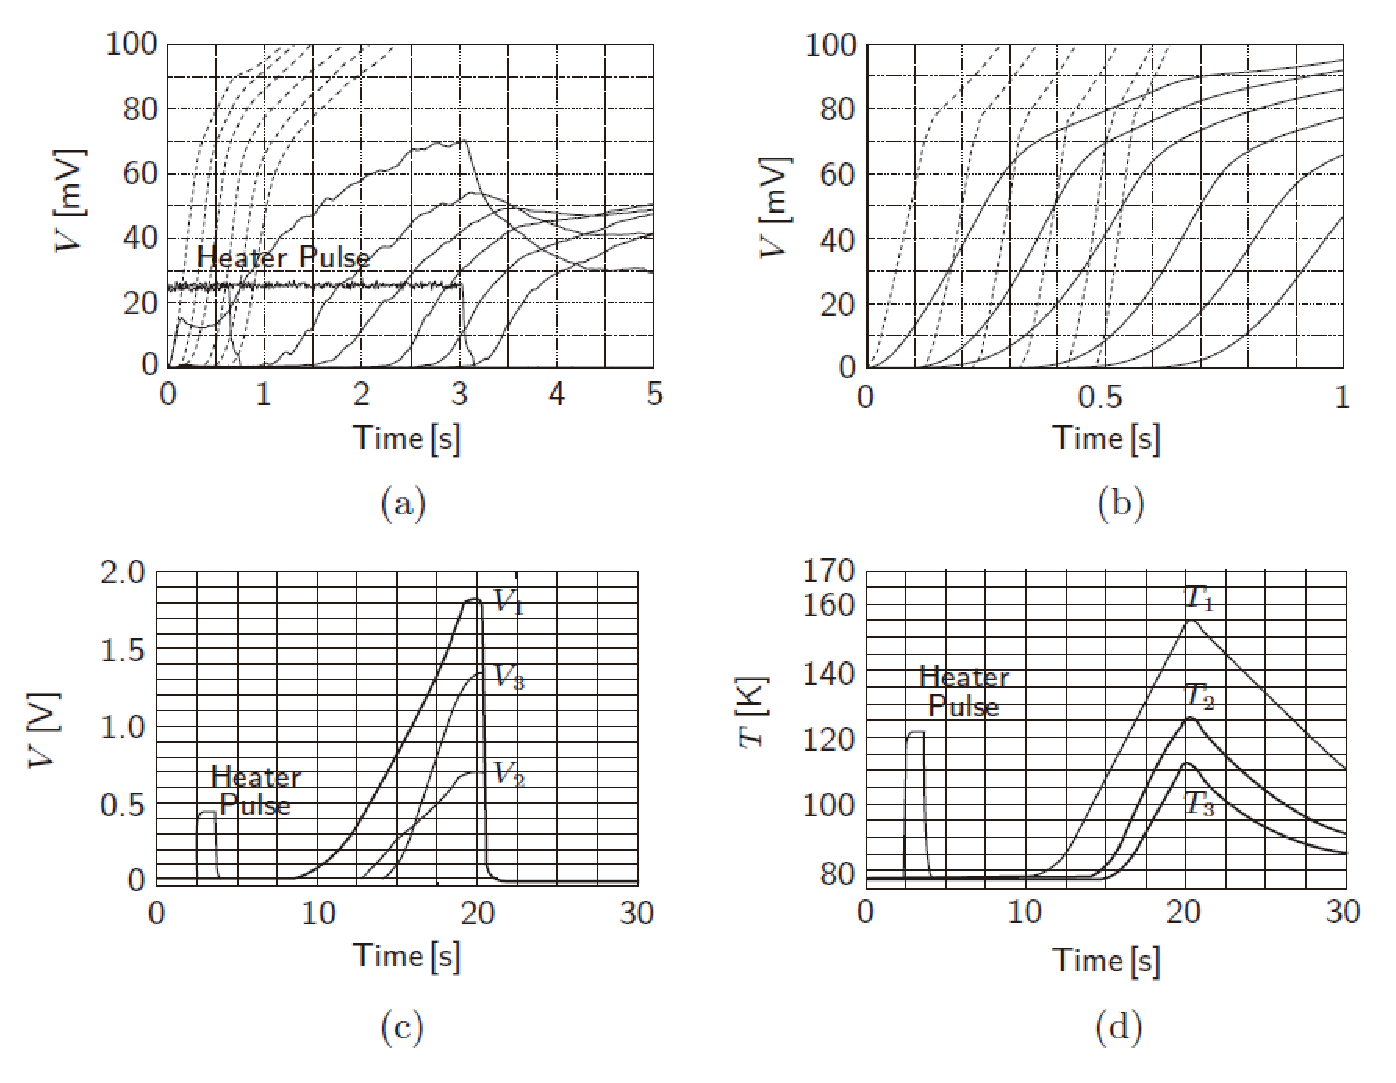
\includegraphics[scale=0.5]{chpt8/figs/fig8.11.eps}
	\caption{YBCO测试样品在77 K时得到的横向NZP信号,失超是由加热脉冲触发的。}
\end{figure}



\subsection{热-流体失超恢复(THQB)}
对于迫流氦冷却的CIC导体,在局部正常区传播速度比迫流氦快时,
会出现热-流体失超恢复(thermal-hydraulic quenchback, THQB)现象。
Luongo等[8.76–8.78; 1.23]最初将之视为CIC导体中失超的其他现象
(内部压力升高、导体末端氦排除等)有关系的一种现象。它通常发生于CIC导体运行在基底电流密度$J_m$
很高,接近导体临界电流的时候。
如讨论6.6将讨论到的,因为在聚变磁体中---CIC导体最重要的大型应用---
CIC导体设计运行在小于$I_m$(方程6.30)良好冷却区间,THQB应该不会成为严重的保护问题。

\subsection{交流损耗诱导的NZP}
到目前为止,我们将焦耳损耗视为绝热绕组中NZP的唯一源。
当非恢复正常区产生并进入故障模式后,磁体电流随时间衰减,衰减电流幅值在$\sim 100$ A/s,进而在绕组中产生时变磁场$dB/dt$---NMR磁体的情况将在问题8.6研究。
时变磁场的存在导致交流损耗的产生;方程6.1中,$g_d(t)\neq 0$。
在没有局部冷却的时候,这个$dB/dt$感应的$g_d(t)$导致在绕组中$\Delta T_{op}>0$。
$g_d(t)$越大,$\Delta T_{op}>0$越大。如6.2.6所述,甚至绝热绕组也能承受一个极限$\Delta T_{op}$,
具体可高至温度裕度极限$[\Delta T_{op}]_{mx}$。
因为这个$g_d(t)$加热,一些NMR磁体以很慢的速率励磁,某些时候会经历一个星期才达到运行电流,
以确保满足绝热稳定性条件$\Delta T_{op}<[\Delta T_{op}]_{mx}$。

因此,$dB/dt$感应的加热令$U_\ell$和$U_t$的视在值明显大于仅有焦耳耗散作为驱动力的NZP。
$dB/dt$感应的加热可以设计用来加速故障事件下的NZP,此时快速扩大正常区并将电流快速降低是很重要的[8.79-8.81]。
为了保护,一些NMR和MRI磁体还使用特殊选定的长绞合节距多丝导体来提高耦合损耗。

在更大的电流衰减率幅值下,比如$\sim 0.1-1$ MA(尽管明显不可能在高感性MRI和NMR磁体中出现,
但在电阻性设备比如限流器中会遇到),Vysotsky等人发现快速NZP接近 1km/s[8.82];
在这种快速电流变化下,失超成为全局的,而不是从局部开始传播的。


\section{计算机仿真}
由于绝热磁体中失超过程的耦合特定,特别是那些多线圈系统,失超分析最好借助计算机来进行。
Wilson在1968年做了早期尝试[8.83],失超仿真工作(一些还引入了实验结果)持续进行[1.5–1.23;8.84–8.100],
一些工作专门针对HTS绕组。

这里我们简要描述FBNML涉及的绝热、螺管绕组的失超仿真程序,该程序的最初工作是1985年Williams[8.101]做的。
FBNML程序简单的认为绕组内控制正常区域传播的复杂热扩散过程可以简化为一个单一参数横向传播速度$U_t$,该参数
依赖于磁场、温度和基底电流密度。
将绕组的热属性的复杂效应归结为$U_t$,极大的简化了程序且没有牺牲很大的准确性[8.45,8.101]。
如8.4.3中讨论的,$U_t$与长度方向的传播速度$U_\ell$有关;
于是,$U_t$在绕组内既与时间有关,也与位置有关。

图8.12给出了绝热螺管绕组内的失超传播示意图,图中的绕组为圆线密排六边形并浸渍了环氧。
图中的失超开始于绕组中平面的最内半径处。
因为下面的对多数磁体都成立的条件,
横向传播速度$U_t$确定的匝间输运时间或通常小于由长度方向传播速度$U_\ell$确定的周向输运时间:
\begin{equation}% 8.56
\frac{d_{cd}}{U_t}\ll\frac{2\pi a_1}{U_\ell}
\end{equation}

\begin{figure}
	\centering
	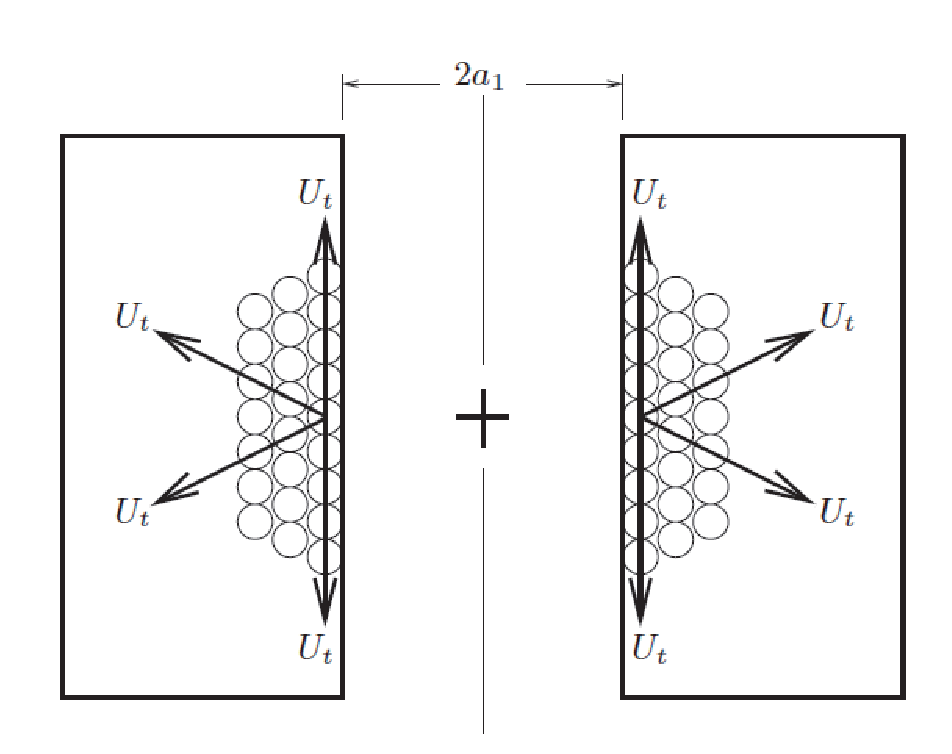
\includegraphics[scale=0.5]{chpt8/figs/fig8.12.eps}
	\caption{绝热螺管绕组中的失超}
\end{figure}

\section{自保护磁体}
如果超导磁体在过热时无需依赖于外部干预即可将正常区域快速扩展到整个绕组,那就称为是自保护的。
根据8.1.2,多数绝热磁体为了保证最高温度低于$\sim 200$ K,至少需要$\sim 10\%$的绕组体积来吸收磁能。
该过程发展的发生快慢可以用NZP速度来衡量。
下面的定性分析将表明,自保护磁体必须有很快的NZP速度且很小。
不过,如后面将讨论的,磁体尽管可以对过热自保护,但不一定能对应力过大保护。

\subsection{尺寸限制}
由8.1.2中的标8.1可见,磁体的初始储能如果完全耗散为绕组中的热量,
为了保持$T_f$在$\sim$200 K以下,绕组的至少$\sim 10\%$($f_r=\sim 0.1$必须
在电流衰减时间$\tau_{dg}$内转变为正常态来吸收能量。

如果在磁体的最内半径$a_1$处产生小正常区,我们需要满足磁体绕组半径$a_1(\alpha-1)$的理想要求来
确保$f_r$足以实现自保护。条件如下:
\begin{equation}% 8.57
\frac{a_1(\alpha-1)}{U_t}<\tau_{dg}
\end{equation}

方程8.57表明整个径向的传播时间$a_1(\alpha-1)/U_t$必须小于$\tau_{dg}$。
实际上,如前所述,不太大的绕组体积分数即足够保持$T_f$在$\sim 200$ K之下。
在这里的“幅值量级”讨论中,我们使用8.57给出的理想条件。

\subsubsection*{恒电流加热下的尺寸限制}
在绝热、恒电流加热模式(8.2.1)下,我们有$\tau_{dg}=\tau_{ah}^i(T_f,T_i)$,其中
$\tau_{ah}^i(T_f,T_i)$由8.12a给出,是绝热恒电流($J_{m_o}$)加热下的最长时间。联立8.57和8.12a,有:
\begin{equation}% 8.58
\frac{a_1(\alpha-1)}{U_t}=\frac{Z(T_f,T_i)}{J_{m_o}^{2}}
\end{equation}

联立8.51b和8.52和8.58,并令$J_m=J_{m_o}$,我们得到绝热恒电流加热条件下的自保护磁体的
绕组尺寸极限$[a_1(\alpha-1)]_{ah}^i$:
\begin{equation}% 8.59
[a_1(\alpha-1)]_{ah}^{i}=\frac{Z(T_f,T_i)}{J_{m_o}C_m(\tilde{T})}\sqrt{\frac{\rho_m(\tilde{T})k_i(\tilde{T})\delta_{cd}}{2\delta_i(T_t-T_{op})}}
\end{equation}

方程8.59表明,允许的磁体尺寸随$J_{m_o}$和$C_m(\tilde{T})$而减小,随$Z(T_f,T_i)$而增大。
它还表明,尺寸极限随$\rho_m(\tilde{T})$和$k_i(\tilde{T})$而增大,随$(T_t-T_{op})$而缩小。
$C_m(\tilde{T})$和$(T_t-T_{op})$的依赖性意味着对同样的$J_{m_o}$和$T_f$,
自保护HTS磁体如果要可以实际应用的话,必须要比LTS更为紧凑才行。

\subsubsection*{端子短接磁体的尺寸限制}
从保护的角度看,让端子短接磁体可以自保护是很有价值的。
实际上,多数NMR和MRI磁体都设计为自保护的。自保护不一定用NZP扩散正常区,而是用
感应交流损耗和二连接于磁体端子的二极管和电阻器。

这里,我们使用仅用NZP的端子短接磁体实现自保护的尺寸极限:
磁体在端子短接下的绝热加热见8.2.3的讨论。
这里,$\tau_{dg}=R_{nz}/L$,其中$R_{nz}$有方程8.27或8.25给出。
联立8.57和8.27,使用8.52和8.51b给出的$U_t$,
解得端子短接自保护磁体在绝热加热时的绕组限制$[a_1(\alpha-1)]_{ah}^{sh}$:
\begin{subequations}% 8.60a 8.60b 8.60c
	\begin{align}
[a_1(\alpha-1)]_{ah}^{sh}=&U_t\left(\frac{L}{R_{nz}}\right) \\
=&\frac{J_{m_o}}{C_n(\tilde{T})}\sqrt{\frac{\rho_m(\tilde{T})k_i(\tilde{T})\delta_{cd}}{2\delta_i(T_t-T_{op})}}\left(\frac{L}{R_{nz}}\right)  \\
=&\frac{J_{m_o}}{C_n(\tilde{T})}\sqrt{\frac{\rho_m(\tilde{T})k_i(\tilde{T})\delta_{cd}}{2\delta_i(T_t-T_{op})}}\times \\\notag
&\frac{4A_m}{f_r\pi(\alpha+1)\rho_m(T_f)}\sqrt{\frac{\mu_o\mathcal{L}(\alpha,\beta)L}{a_1}}\\
[a_1(\alpha-1)]_{ah}^{sh}=&\frac{1}{C_m(\tilde{T})}\sqrt{\frac{\rho_m(\tilde{T})k_i(\tilde{T})\delta_{cd}}{2\delta_i(T_t-T_{op})}}\times \\\notag
&\frac{4}{f_r\pi(\alpha+1)\rho_m(T_f)}\sqrt{\frac{2\mu_o\mathcal{L}(\alpha,\beta)E_m}{a_1}}
\end{align}
\end{subequations}

类似的,在如上面处理的恒电流加热模式下,因为$C_m(\tilde{T})$和$(T_t-T_{op})$出现在8.60c和8.60d的分母中,
在同样的运行参数下,自保护HTS磁体必须要比运行于液氦温度的LTS尺寸更小。


\section{“孤立”磁体的被动保护}
被动保护技术通常用于持续模式超导磁体,如NMR和MRI。
不像8.8中所讨论的主动保护技术,被动保护通常不依赖于低温容器外部的设备。

图8.13给出了持续模式磁体的电路模型,其中磁体由两个串联的电感表示。
它采用了最简单的模型,实际磁体通常有很多嵌套的线圈。
磁体被持续电流开关PCS旁路,开关的状态在加热电流存在时为“正常态”,在加热器关闭后为超导态。
(本电路不包括保护PCS的二极管,含二极管的更完整的电路如图7.22所示。
包含保护二极管的持续模式电路运行的基本特征将在讨论7.8中描述。)
这个模型中,各线圈均有旁路电阻($R_1$或$R_2$)。电阻是孤立磁体保护的关键元件。

在这个简单系统中,各线圈的自感是一致的:$L_1=L2=L$;
互感为$M=k\sqrt{L_1L_2}=kL$,其中$k$是耦合系数;
同时还有$R_1=R_2=R$。
起始,各线圈载有恒定传输电流$I_0$。
时刻$t=0$,线圈1内形成了小正常区;它由一个定值小电阻表示(图8.13未画出)。

系统的总磁能为:$E_m=(L+M)I_0^2$。
电阻$r$上耗散的总磁能与系统总磁能之比$E_r/E_m$用$\zeta=r/R$表示为:
\begin{equation}% 8.61
\frac{E_r}{E_m}=\frac{0.5\zeta(1-k)+(1+k)}{\zeta+(1+k)}
\end{equation}

\begin{figure}
	\centering
	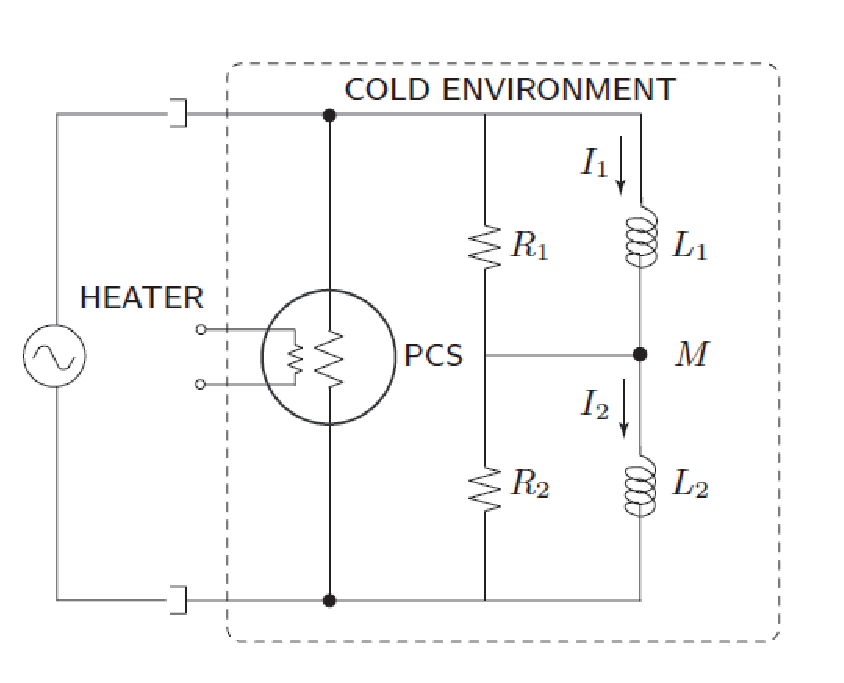
\includegraphics[scale=0.6]{chpt8/figs/fig8.13.eps}
	\caption{“孤立”的持续模式2线圈磁体的电路模型。}
\end{figure}

多数高性能线圈都能满足$r\gg R(1+k)$条件,此时给出的$I_1(t)$和$I_2(t)$为:
\begin{subequations}
	\begin{align}
\frac{I_1(t)}{I_0}=&\frac{R(1+k)^2}{2r}\exp\left(-\frac{Rt}{2L}\right)\left[1-\frac{R(1+k)^2}{2r}\right]\exp\left[-\frac{rt}{(1-k^2)L}\right]\\
	\frac{I_2(t)}{I_0}=&(1+k)\exp\left(-\frac{Rt}{2L}\right)-k\exp\left[-\frac{rt}{(1-k^2)L}\right]
	\end{align}
\end{subequations}

由8.62,我们可以得到如下结论:
\begin{itemize}
		\item 方程8.61表明,当$r\rightarrow 0$时,$E_r/E_m\rightarrow 1$。
		这是由于为了将能量转移到旁路电阻---唯一的可以用于吸收耗散能量的元件---
		必须在各旁路电阻上形成电压。
		如果正常区域电阻$r$很小,旁路电阻$R_1$上的电压也很小。
		当$r\rightarrow 0$时,各旁路电阻上仅有很小的电压,而整个磁场能量被正常区耗散,从而$E_r/E_m\rightarrow 1$;
		幸好,这种情况不会发生于绝热绕组,因为在绝热绕组中一旦形成正常态区域,$r$迅速增加,在各旁路电阻上提供
		足够的电压。
		\item 方程8.61还表明,当$r\rightarrow\infty$时,$E_r/E_m\rightarrow 0.5(1-k)$,$k=1$意味着
		$E_r/E_m=0$。在这个条件下,各旁路电阻上出现很高的电压,总能量的大部分耗散于旁路电阻上。
		如果两个线圈耦合很好$(k\rightarrow 1)$,储存与线圈1的能量被转移到线圈2,通过旁路电阻耗散。
		
		注意到因为跨过两个旁路电阻的总电压必须总是为零,两个旁路电阻中必然流过相同(但反向)的电流;
		两个电阻的耗散相同。也即,若$R_1=R_2$,则各旁路电阻耗散相同的能量。
		\item 方程8.62b给出,在$r/R\gg (1-k^2)/2$时,仍处于超导态的线圈2的电流$I_2(t)$开始增加。
		线圈1中出现的$r$迫使电流流过旁路电阻$R_1$。
		因为磁体端子之间的电压必须为零---PCS是超导态---
		在旁路电阻$R_2(=R_1)$中必须流过一个相等但反向的电流。
		各旁路电阻中的电流最终会进入线圈2,导致$I_2(t)$增加,$I_1(t)$则减少相同的电流,保持磁体中磁通不变。
		\item $I_2(t)$的增加一致持续到它达到超导体在线圈中平面处最内层绕组半径处临界电流,
		导致线圈2失超,这会促进正常区的快速扩展。
		这个过程将在下一个问题中进一步考察,届时我们将更细致的研究一个真实的线圈工况。
		\item  有利于触发失超的$I_2(t)$大幅度增加可能带来问题。因为如上所述,磁通保持不变,
		这导致绕组中应力大幅升高。这意味着设计使用旁路电阻保护的线圈时,他们必须设计具有承受失超中可能
		出现的最大应力的能力。
		失超过程中的一个重要参数是$I_2(t)\times B_2(t)$。
	\end{itemize}

\subsubsection*{两线圈磁体}
作为一个实例,这里研究如图8.14所示的两线圈磁体。
两个串联的线圈均由带绝缘的NbTi导线绕成(密排六边形),各线圈分别并联0.5 $\Omega$旁路电阻。
电源可以建模为最高电压10 V的恒流源。

分析中,我们假设正常区传播主要由横向热传导决定。
正常区在整个圆周上沿径向和轴向三维扩大。
尽管因为$2\pi a_{1_1} U_\ell d_1 U_t$(其中$a_{1_1}$和$d_1$分别是线圈1的内绕组半径和导体直径。),
导致$U_\ell\gg U_t$,但横向传播在两部分都是主要部分。

表8.6给出了线圈参数。总电感是1.52 H。
因为线圈2是直接绕在线圈1上的,两线圈界面上的热接触良好:整个线圈可以视为均一的热单元。(如表8.6所给的,
两个线圈的导线直径不同,于是NZP速度不同。)

线圈1中平面上最内直径处放置一个用于制造失超的加热器。
于是,我们可以结社正常区开始于线圈1中平面上最内直径的环上,如图8.12那样扩展到线圈2。

图8.15给出了加热器驱动的失超的电流电压随时间变化的曲线,该磁体初始电流100 A;
电源电压极限为10 V。
电流和电压图都包含四条线:实线(实验)和虚线(仿真)。
电流和电压曲线中,标为1的表示第1部分,标为2的表示第2部分。
在回答下列问题时,可以忽略分析曲线。

\begin{itemize}
\item 从图8.15曲线中,可以得到如下结论:
	\begin{enumerate}
		\item  因为第1部分最早出现失超,$I_1$首先下降。
		\item $I_2$开始上升以保持磁通不变。
		\item $I_1$和$I_2$的行为也反映在$V_1,V_2$上。
		$V_2$升高,因为$\Delta I_1$不是通过第1部分,而是通过$R_1$。
		\item 为保持端子电压为0(至少在初始时),$V_2$变为负的。这些初始响应与问题8.9的结果一致。
		最终$V_1+V_2$爬升至电源极限10 V。
		\item 在$t\sim$0.2 s,$V_2$开始爬升,明确表明正常区域已经进入线圈2。
		\item $I_2$因此开始下降,$I_1$升高,以保持磁通不变。
		\item 在$t\sim$0.4 s,$V_1+V_2$达到10 V,$I_1$必须开始下降。
		\item 在$t>$0.4 s后,$V_1+V_2=10$ V。
	\end{enumerate}
\item 磁体中耗散的总能量$E_d$可由下式给出:
\begin{equation}% 8.63
E_d=E_m+E_s-E_{R1}-E_{R2}
\end{equation}
式中,$E_m$是磁体初始的总储能量,$E_s$是$t=0$到$t=2$ s时间内电源提供的能量,
$E_{R1}$和$E_{R2}$分别是耗散于$R_1$和$R_1$的能量。
$E_m$=7600 J$[(0.5)(1.52)(100)^2]$。
$E_s$由$V_s(t)I_s(t)$在$0\le t\le 2$之间的积分得到。
$V_s(t)$和$I_s(t)$分别是电源的电压和电流。
电源在$0\le t\le$0.4 s间可以建模为恒流源(100 A),$t\ge 0.4$ s后,可以建模为恒压源(10 V)。
在$0\le t\le$0.4 s,我们有$V_s(t)=V_1(t)+V_2(t)$,在$t\ge 0.4$ s,有$I_s(t)=I_1(t)+I_2(t)/R_1$。
(涉及更多线圈的类似关系的证明见问题8.11.)

使用图8.15中的曲线,我们计算$E_s,E_{R1}$和$E_{R2}$:
\begin{align*}
E_s&=(100\ \mathrm{A})\int_{0}^{0.4\ \mathrm{s}}[V_1(t)+V_2(t)]dt+(10\ \mathrm{V})\int_{0.4\ \mathrm{s}}^{2\ \mathrm{s}}\left[I_1(t)+\frac{V_1(t)}{R_1}\right]dt \\
&\simeq 200\ \mathrm{J}+650\ \mathrm{J}\simeq 850\ \mathrm{J}\\
E_{R1}&=\frac{1}{R_1}\int_{0}^{2\ \mathrm{s}}V_1(t)^2dt\simeq 50\ \mathrm{J} \\
E_{R2}&=\frac{1}{R_2}\int_{0}^{2\ \mathrm{s}}V_2(t)^2dt\simeq 300\ \mathrm{J}
\end{align*}
于是,磁体中耗散的总磁能约为5500 J。

\item 如果$I_0=50$ A,正常态将在$\sim 0.4$ s或更晚达到线圈2,因为$U_t\propto U_\ell\propto I_t$。
同时,$B$减半或$T_c$提高使达到时间比0.4 s更晚。
因为旁路电压降低2分之一,端子电压达到10 V所需的时间会更长:长于0.4 s,或许长达0.8 s。

\item 总绕组体积(导体和环氧填充物)是694 $\mathrm{cm^3}$。假设全绕组的热容$C_{wd}$以铜代表,有:
\begin{align*}% page500第四个
\mathcal{V}_{cd}[h_{cu}(T_f)-h_{cu}(T_{op})]\simeq(694\ \mathrm{cm^3})[h_{cu}(T_f)]=5500\ \mathrm{J}
\end{align*}
其中,$\mathcal{V}_{cd}$是绕组体积,$h_{cu}$是铜的单位体积焓。
$T_f>T_{op}=4.2$ K时,$h_{cu}(T_f)\gg h_{cu}(T_{op})$。
从图A3.3中,我们发现$T_f\simeq$50 K,与47 K(图8.16)仿真数据大致吻合。

\item 使用铝替换铜,图A3.3给出$T_f=75$ K。仿真给出的温度是57 K。
\end{itemize}


\begin{figure}
	\centering
	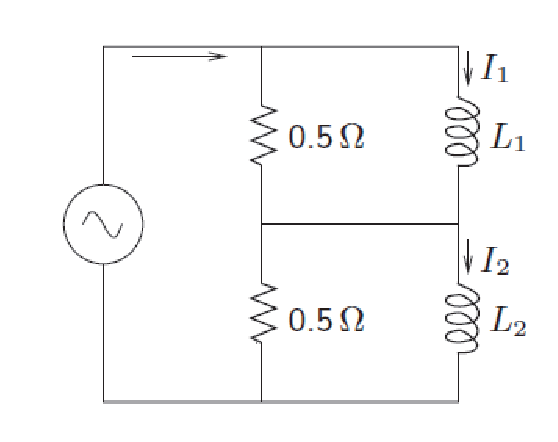
\includegraphics[scale=0.6]{chpt8/figs/fig8.14.eps}
	\caption{两线圈磁体电路模型}
\end{figure}

表8.6.。。。。。。。。。。。。。。。

\begin{figure}
	\centering
	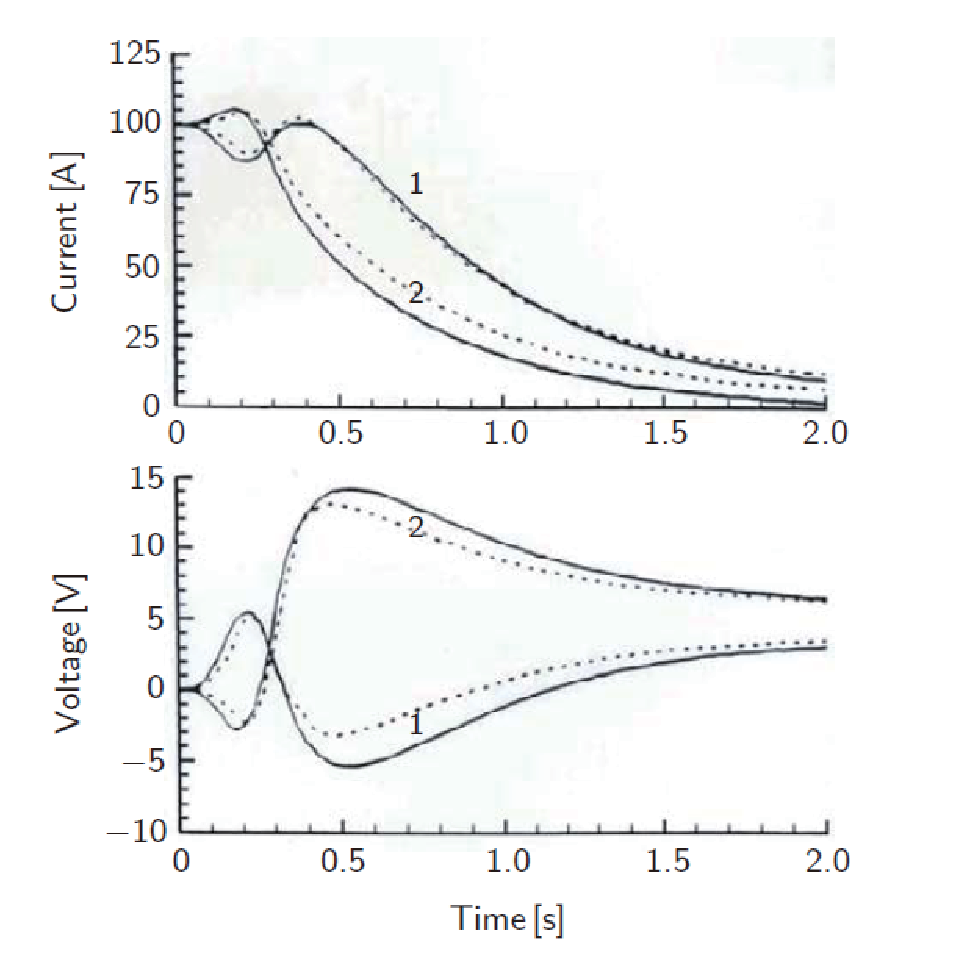
\includegraphics[scale=0.5]{chpt8/figs/fig8.15.eps}
	\caption{线圈1(标号1)和线圈2(标号2)的电流电压的时间曲线):实验值为实线,仿真值是虚线。 }
\end{figure}

图8.16给出了磁体的第1部分和第2部分的空间平均温度。实线对应的是NbTi/Cu导线,
虚线对应的是NbTi/Al导线[8.46]。

\begin{figure}
	\centering
	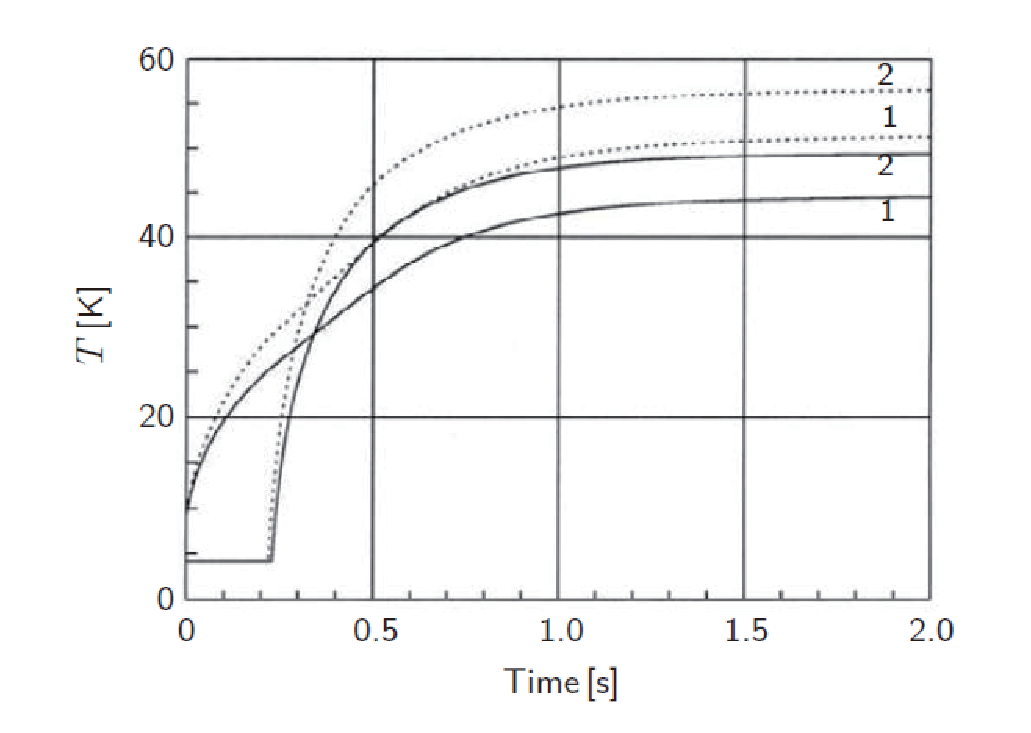
\includegraphics[scale=0.6]{chpt8/figs/fig8.16.eps}
	\caption{磁体的第1部分和第2部分的空间平均温度。}
\end{figure}



\section{主动保护}
\subsection{过热}
除了电力应用的大部分超导磁体都是以磁场储存大量能量的低电压设备。
所以,保护一般意味着确保总能量不被转换为局部绕组的热,
反过来,又通常意味着确保能量吸收区域的最高温度不超过安全水平,比如200 K。

如前论及,自保护磁体通过足够大的NZP速度让绕组在能量转换时间尺度内将能量吸收区域
扩大到大部分绕组来实现上述保护目标。
但是,自保护磁体存在尺寸限制,甚至具有很快NZP速度的LTS高性能磁体也是如此。
因为NZP速度很低,HTS磁体不能自保护。

如8.1所述,磁体保护的一个重要目标就是限制绕组最大温度$T_f$不超过200 K。
自保护磁体通过自身实现上述目标,无需特别为此目的为系统设置额外干预。
与主动保护不同,我们将这种自保护磁体称为是“被动保护”的。

主动保护的基本方法是1) 将存储的大部分能量$E_m$转移到绕组外部;或2) 在绕组的很大部分区域内($f_r\le 0.1$)分布
能量。两种方法都可以实现$T_f<200$ K的目标,这可以从方程8.7看出:
\begin{align*}% page501 8.7
e_{mr}\equiv\frac{E_m}{V_r}=\frac{2(\alpha-1)\beta\mathcal{L}(\alpha,\beta)}{f_r\pi(\alpha+1)F^2(\alpha,\beta)}\left(\frac{B_{o}^{2}}{2\mu_o}\right) \tag{8.7}
\end{align*}

于是,方法1)中,尽管$f_r$很小,绕组中转换为热的有效磁能$E_m$是减小的;
方法2)中,有效磁能$E_m$维持初始储能相同的水平不变,但$f_r$增加。
每一种方法都能降低$e_{mr}$。

\subsection{多线圈磁体中的过应力}
尽管到目前为止尚未论及,仅用于相互耦合的多线圈磁体的保护还有另一个重要目标。
这里,失超导致的一个线圈的电流衰减可能在另一个线圈中感应出很大的电流,
导致线圈中应力超出极限,损坏线圈。(这种电流引起的过应力不同意温度引起的过应力)

我们在两线圈磁体中已经看到了这一点。
如方程8.62b给出的,$I_2(t)/I_0$(线圈2中的电流,线圈1进入正常态后线圈2仍保持超导)开始升高
超过$I_0$,这可能导致线圈2中导体的过应力---
$I_2(t)$的增加还可以从图8.15两线圈磁体系统的录波的电流曲线看出。
本部分将讨论可最小化该电流升高的一种主动保护技术。

\subsection{主动保护技术:检测-泄放}
这种所谓的“检测--泄放”(detect and dump)技术在大型磁体系统中广泛使用。
该技术最初由Maddock和James于1968年[8.3]提出,基本思路是将存储的大部分磁能转移到连接于磁体端子的
泄放电阻器而保护磁体。
这样,哪怕对于很大的$E_m$,$f_r$仍可保持很小。
图8.17给出了检测-泄放技术的基本电路。
磁体由电感$L$代表;泄放电阻由$R_D$代表,连接于磁体的端子,通常位于低温容器之外。
开关S在非恢复正常区(由$r(t)$表示)在磁体中出现时被打开。
在运行电流$I_{op}$下储存的磁能$E_m$为$LI_{op}^2/2$。
一旦开关S打开,电路就和图8.3一致了。在8.2.2中我们已讨论了一些和本技术相关的要点。

由于可能形成危害的大部分能量耗散于别处,
绕组内正常区被加热的时间缩短。这样,限制$T_f$到一个安全水平是可能的:
电流衰减速率越快,热点温度越低。
不过,为了实现快速放电,磁体端子必须承受高电压。
于是,磁体设计者试图同时限制温度$T_f$和端子电压$V_D$:两者在很多情况下是竞争性的要求。
$T_f$(以$Z(T_f,T_i)$形式)和$V_D$和(其他参数)的关系已在8.2.2讨论,可由方程8.18b表示:
\begin{align*}% page502 8.18b
Z(T_f,T_i)=\frac{J_{m_o}E_m}{A_{cd}V_D}\tag{8.18b}
\end{align*}
其中,$J_{m_o}$是运行电流$I_{op}$下的基底电流密度。

\begin{figure}
	\centering
	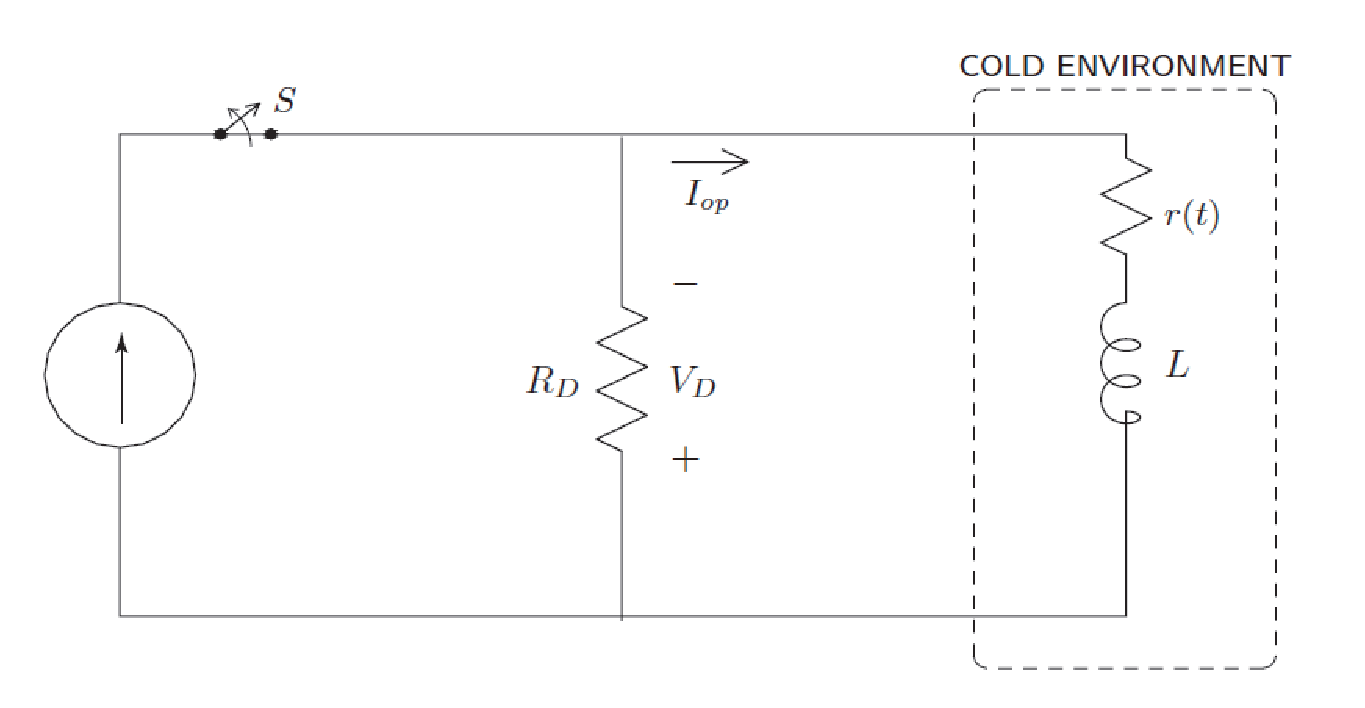
\includegraphics[scale=0.5]{chpt8/figs/fig8.17.eps}
	\caption{检测-泄放主动保护的磁体电路模型。}
\end{figure}

上述内容可归结为运行电流下基底金属电流密度$J_{m_o}^D$的一个过热判据,如方程8.19给出:
\begin{align*}% page503 8.19
J_{m_o}^{D}=\frac{A_{cd}Z(T_f,T_i)V_D}{E_m}\tag{8.19}
\end{align*}

这种主动保护技术要求两个相继的执行动作:
1) 非恢复正常区(可能很小)检测;2)打开开关S,迫使磁体通过泄放电阻放电。
本技术的缺点是上述两个动作都可能不可靠。
正常区的检测并不简单,这是因为检测通常需要在磁体充电过程中存在高电压时
而不是它已充电到$I_{op}$时的准静态下进行。
此种保护技术有用的失超电压检测方法将在后面讨论。

\textbf{提高$J_{m_o}^D$的方法}\quad 方程8.19指出,在给定的$\gamma_{m/s}, T_f$和$E_m$下,
提高$J_{m_o}^D$的方法有两种:提高$A_{cd}$和/或$V_D$。
$A_{cd}$的提高引起$I_{op}$提高。
从图8.2可知,在所给出的基底金属中,Ag1000的$Z(T_f,T_i)$最大。
为了提高$J_{m_o}^D$,相比于铝和黄铜,青铜和银作为基底金属更合适。

提高$A_{cd}$(增加$I_{op}$):这个方法需要评估以下后果:
\begin{enumerate}
	\item 给定kA-m下的大型导体通常比小型导体更贵。
	\item 大电流引线会导致进入低温容器的热量更多。
	\item 电流引线和母线系统的大$\vec{B}\times \vec{I}$力。
	\item 在给定功率$VI$下,大电流电源通常比小电流电源更贵。	
\end{enumerate}

提高$V_D$:这明显会增加液氦浸泡磁体放电的可能性,特别是当$V_D$超过$\sim 700$ V的时候。

\textbf{放电电压$V_D$}

在给定的$Z(T_f,T_i)$下,从8.18可以看到,有5个设计参数:$J_{m_o};E_m,\gamma_{m/s};V_D$和$I_{op}$。
于是:
\begin{equation}% 8.65
V_D=\frac{J_{m_o}E_m}{A_{cd}Z(T_f,T_i)}
\end{equation}
上式表明,$V_D$随$E_m$和$J_{m_o}$线性增加,随$A_{cd}(I_{op})$和$Z(T_f,T_i)$成反比减小。

\textbf{开断延迟}

方程8.18和8.19都假设了非恢复区产生后放电立即开始。实际上,两者之间存在一个延迟$\tau_{dl}$:
$\tau_{dl}$是正常区检测延迟和开断实际打开的电路延迟之和。
在延迟期间,电流保持初始值$I_{op}$。
所以,为了通过$Z(T_f,T_i)$计算$T_f$,我们应该在方程8.12a中代入延迟$\tau_{dl}$取代$\tau_{ah}^i(T_f,T_i)$,并与8.16a联立:
\begin{subequations}
	\begin{align}
Z(T_f,T_i)&=\left(\frac{A_m}{A_{cd}}\right)(J_{m_o}^{2}\tau_{dl}+\frac{1}{2}J_{m_o}^{2}\tau_{dg})\\
&=\left(\frac{A_m}{A_{cd}}\right)(\tau_{dl}+\frac{1}{2}\tau_{dg})J_{m_o}^{2}
	\end{align}
\end{subequations}

\subsection{主动保护技术:检测-激活加热器}
这个“检测-激活加热器”技术广泛用于大型磁体[8.102-8.110]。
在检测磁体电阻区的时候,绝大部分,至少很大部分的仍处于超导态的绕组通过保护加热器而被驱至正常态。
加热器安装在绕组中,强迫增加$f_r$。
如表8.1所示,对多数磁体,$T_f<200$ K的目标在$f_r<0.1$下可以实现,此时在绕组中安装一个保护加热器
要比在$f_r$接近1的情况下更轻便。
同时看到,保护加热器可以安装在绕组的便于安装的位置,与失超点或其初始大小关系不大[8.75,8.111]。
这个可以将保护加热器安装于便于安装的位置的概念在讨论8.6中会深入讨论。

\subsubsection*{被动激活加热器}
\begin{figure}
	\centering
	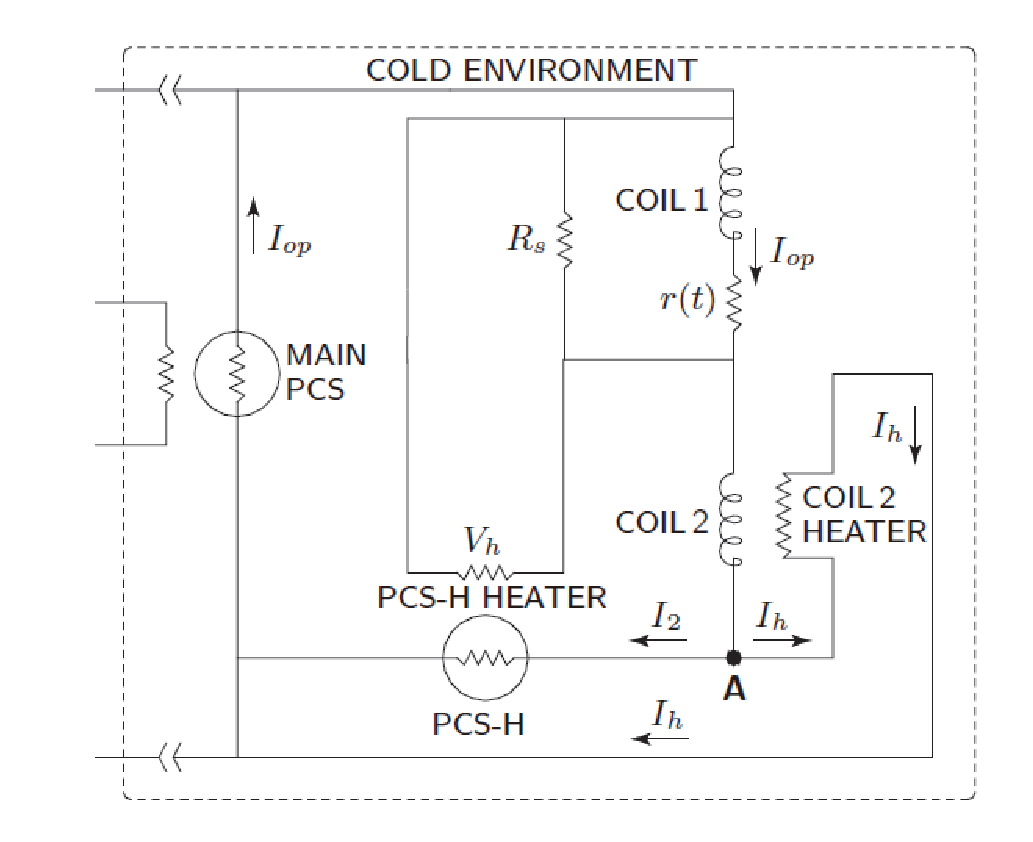
\includegraphics[scale=0.6]{chpt8/figs/fig8.18.eps}
	\caption{带有被动激活加热器保护的磁体电路图。}
\end{figure}

图8.18给出了带有被动激活加热器保护的两线圈持续模式(“孤立”)磁体的电路图。
该电路是持续模式NMR磁体[8.101]的简化版。实际NMR磁体由嵌套线圈组成,各线圈均有旁路电阻;
这里为了简化,电路仅给出一个旁路电阻$R_s$。
在这个两线圈版本中,线圈2(插入线圈1中)上绕制了加热丝(线圈2加热器)。
在正常运行条件下,线圈1中有$r(t)=0$:
$I_1=I_{op};I_h=0;V_h=0$。其中$I_h$是线圈2加热器的电流。
当线圈1失超后,$r(t)\neq 0$,PCS-H加热器上出现电压$V_h$,PCS-H成为电阻性而“打开”。
点A处。磁体电流$I_{op}$的大部分转移至线圈2的加热器中,有$I_h>0(I_2+I_h=I_{op})$,
在线圈2的最外层产生正常态区域。

这种检测-激活加热器保护的被动版本是适合持续模式磁体的,因为基于电压的失超监测不可能也不要求。
监测-激活加热器技术有多种变体。



\subsection{失超电压检测技术---基本电桥电路}
执行主动保护的一个关键过程是非恢复失超的检测。
主动保护通常强迫磁体放电,该过程会中断磁体运行:必须避免假警报放电。
在充满噪声的实际环境中检测真实的失超电压充满挑战[8.112,8.113]。

图8.19给出了包括两个串联线圈1和线群2两个线圈的基本电桥电路。
两个线圈实际中可以是分为两个部分的同一个线圈。
$L_1$和$L_2$分别是线圈1和线圈2的自感(本模型中,由于两线圈串联,两线圈间的互感可以包括自感中去)。
$r$表示线圈1失超产生的小正常区。$R_1$和$R_2$是电桥电阻,$V_{out}(t)$表示电桥输出。

\begin{figure}
	\centering
	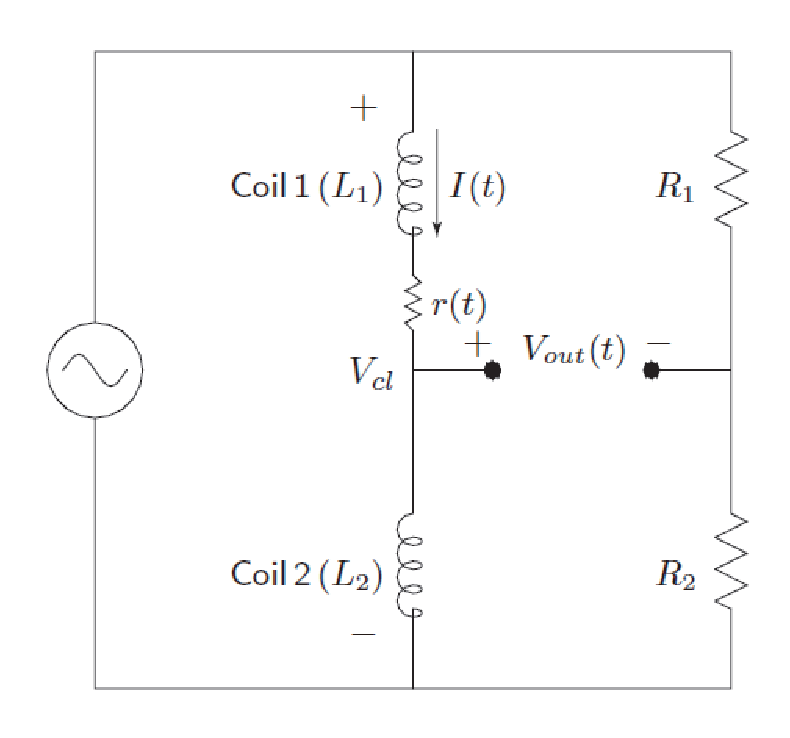
\includegraphics[scale=0.6]{chpt8/figs/fig8.19.eps}
	\caption{电桥电压检测技术。}
\end{figure}

下面的分析中,我们假设包括$r$在内的所有的电路元件都是不变的;
同时,我们假设$R_1$和$R_2$足够大,不会影响电桥电路负载。

在$R_1$和$R_2$很大时,两线圈上的总电压$V_{cl}(t)$由下式给出:
\begin{equation}% 8.67a
V_{cl}(t)=L_1\frac{dI(t)}{dt}+rI(t)+L_2\frac{dI(t)}{dt}
\end{equation}
同样条件下,通过$R_1$和$R_2$的电流$i_R(t)$由下式给出:
\begin{align*}% 8.67b
i_R(t)=\frac{V_{cl}(t)}{R_1+R_2} \tag{8.67b}
\end{align*}
从图8.19的电路中,我们有:
\begin{align*}% 8.67c
V_{out}(t)=L_1\frac{dI(t)}{dt}+rI(t)-R_1i_R(t) \tag{8.67c}
\end{align*}

联立上面三式,我们有:
\begin{align}% 8.68
V_{out}(t)=&L_1\frac{dI(t)}{dt}+rI(t) \\
&-\frac{R_1}{R_1+R_2}\left[L_1\frac{dI(t)}{dt}+rI(t)+L_2\frac{dI(t)}{dt}\right] \\\notag
=&\left(\frac{R_2}{R_1+R_2}\right)L_1\frac{dI(t)}{dt} \\
&-\left(\frac{R_1}{R_1+R_2}\right)L_2\frac{dI(t)}{dt}+\left(\frac{R_2}{R_1+R_2}\right)rI(t)
\end{align}

为了使$V_{out}(t)$仅正比于$rI(t)$,方程8.69等号右侧前两项必须为零:
\begin{equation}% 8.69
\left(\frac{R_2}{R_1+R_2}\right)L_1\frac{dI(t)}{dt}-\left(\frac{R_1}{R_1+R_2}\right)L_2\frac{dI(t)}{dt}=0
\end{equation}

化简方程8.69得到以下条件:$R_2L_1=R_1L_2$。
8.68消去前两项,成为:
\begin{equation}% 8.70
V_{out}(t)=\left(\frac{R_2}{R_1+R_2}\right)rI(t)
\end{equation}

我们在讨论8.1中将看到,实际混合磁体中的条件远非理想情况:
实际磁体中通常很难实现与$I(t)$和$dI/dt$无关的$R_2L_1=R_1L_2$。

专题中,上面的论及的部分问题将会进一步深入研究,有些给出精细的结论。

\section{专题}

\subsection{问题8.1:大型超导磁体的回温}
超导磁体的测试过程中,将之从低温4.2 K回温到室温通常是很必要的。
如果浸泡于制冷剂的磁体是小的,我们可以简单的排空低温容器中的制冷剂后不管它,
等待几个小时到几天的时间,磁体即可回温到室温。

本问题中,我们考虑两种回温大型磁体的方法。首先考虑一个在4.2 K液氦中运行的磁体,
接下来考虑一个在77 K液氮中运行的磁体。
对一个液氦浸泡的大型磁体,常用的方法是将磁体端子连接到电源上加热磁体。
这里,我们考虑两种电源:1) 恒流源(8.2.1);2) 恒压源(8.2.4)。

回温过程可以用下面的微分方程描述,其中$T$是磁体温度。
\begin{subequations}
	\begin{align}
\mathcal{V}C_{cd}(T)\frac{dT}{dt}=&\frac{\rho_m(T)\ell_{cd}}{A_m}I_{o}^{2} \\
=&\frac{A_m}{\rho_m(T)\ell_{cd}}V_{o}^{2}
	\end{align}
\end{subequations}
式中,$\mathcal{V}_{cd}$是磁体全部导体的体积,这里假设热仅存储与导体中;
$C_{cd}(T)$是导体热容,这里假设等于铜的热容,$C_{cd}(T)=C_{cu}(T)$;
$\rho_m(T)$是铜的电阻率,$\rho_m(T)=\rho_{cu}(T)$;
$\ell_{cd}$是磁体中导体总长度;
$A_m$是铜的横截面积;
$I_o$是恒流源的电流;
$V_o$是恒压源的电压。

假设在两种加热模式下,磁体都没有其他热输入源。
(有时候,会破坏低温容器真空以加速回温过程,但这种操作一般不推荐:它会导致容器表面结霜,
很难看。在CIC磁体中,可以通过在绕组内循环氦气促进回温过程。)

对这个特定的磁体:$\mathcal{V}_{cd}=0.4\ \mathrm{m^3};\ell_{cd}=10^4\ \mathrm{m};A_m=1.5\times 10^{-5}\ \mathrm{m^2}$。(多数使用梯度导体的磁体中,$A_m$并不像这里假设的这样在全绕组内都是定值。)

a) 计算当恒流$I_o$=25 A加热时,从10 K回温到300 K的近似($\pm 20\%$不确定性之下)回温时间。

b) 计算当恒压$V_o$=25 V加热时,从10 K回温到300 K的近似($\pm 20\%$不确定性之下)回温时间。

c) 讨论一个实际的案例,由于实际电源的限制,其在整个温度区间,既不是恒流也不是恒压。

d) 重复a),初始温度变为80 K。

e) 重复b),初始温度变为80 K。

\subsubsection{问题8.1之解}
a) 我们可以使用方程8.71a来计算在恒流加热条件下从10 K到300 K的回温时间$\Delta t_w^I|_{10\ \mathrm{K}}^{300\ \mathrm{K}}$:
\begin{align*}% page508 S1.1
\Delta t_{\omega}^{I}\mid_{10\ \mathrm{K}}^{300\ \mathrm{K}}&=\frac{\mathcal{V}_{cd}A_m}{\ell_{cd}I_{o}^{2}}\int_{10\ \mathrm{K}}^{300\ \mathrm{K}}\frac{C_{cu}(T)}{\rho_m{cu}(T)}dT \\
&=\frac{\mathcal{V}_{cd}A_m}{\ell_{cd}I_{o}^{2}}Z(T_f=300\ \mathrm{K},T_i=10\ \mathrm{K}) \tag{S1.1}
\end{align*}

对青铜,RRR=100,图8.2给出的$Z(T_f,T_i)$为:
$Z(T_f=300\ \mathrm{K},T_i=10\ \mathrm{K})=15.1\times 10^{16}\ \mathrm{A^2 s/m^4}$。
解出$\Delta t_w^I|_{10\ \mathrm{K}}^{300\ \mathrm{K}}$,有:
\begin{align*}% page508 S1.2
\Delta t_{\omega}^{I}\mid_{10\mathrm{K}}^{300\mathrm{K}}&=\frac{(0.4\ \mathrm{m^3})(1.5\times 10^{-5}\ \mathrm{m^2})(15.1\times 10^{16}\ \mathrm{A^2s/m^4})}{(1\times 10^4\ \mathrm{m})(25\ \mathrm{A})^2} \\
&\simeq 1.45\times 10^5\ \mathrm{s}\simeq 40\ \mathrm{h}\simeq 1\frac{2}{3}\ \mathrm{days}  \tag{S1.2}
\end{align*}

在恒流25 A下,磁体从10 K到300 K的回温时间略小于2天。

b) 我们可以使用8.71b计算在恒压加热条件下从10 K到300 K的回温时间$\Delta t_w^V|_{10\ \mathrm{K}}^{300\ \mathrm{K}}$:
\begin{align*}% page508 S1.3
\Delta t_{\omega}^{I}\mid_{10\mathrm{K}}^{300\mathrm{K}}&=\frac{\mathcal{V}_{cd}\ell_{cd}}{A_mV_{o}^{2}}\int_{10\ \mathrm{K}}^{300\ \mathrm{K}}C_{cu}(T)\rho_m{cu}(T)dT \\
&=\frac{\mathcal{V}_{cd}\ell_{cd}}{A_mV_{o}^{2}}Y(T_f=300\ \mathrm{K},T_i=10\ \mathrm{K})\tag{S1.3}
\end{align*}

对青铜,RRR=100,图8.6给出的$Y(T_f,T_i)$为:
$Y(T_f=300\ \mathrm{K},T_i=10\ \mathrm{K})=7.25\ \mathrm{V^2 s/m^2}$。
解出$\Delta t_w^V|_{10\ \mathrm{K}}^{300\ \mathrm{K}}$,有:
\begin{align*}% page508 S1.4
\Delta t_{\omega}^{I}\mid_{10\mathrm{K}}^{300\mathrm{K}}&=\frac{(0.4\ \mathrm{m^3})(1\times 10^4\ \mathrm{m})(7.25\ \mathrm{V^2s/m^2})}{(1.5\times 10^{-5}\ \mathrm{m^2})(25\ \mathrm{V})^2} \\
&=3.1\times 10^6\ \mathrm{s}\simeq 860\ \mathrm{h}\simeq 36\ \mathrm{days} \tag{S1.4}
\end{align*}

在恒压25 V下,磁体从10 K到300 K的回温时间大约是36天。

可以算的,10 K时磁体的电阻为$0.32\ \Omega$,在300 K时为$17.2\ \Omega$。
这意味着在25 A的电源下,电压和响应的功率分别为:10 K时为8 V和200 W;300 K时为430 V和$\sim$11 kW。
类似的,在25 V电源下,10 K时为78 A和$\sim 2$ kW;300 K时为$\sim$1.5 A和$\sim$35 W。

大部分恒流电源不能提供无限的电压;同样,大部分恒压源也不能提供无限的电流。
因此,25 A模式的实际回温时间要长于上面计算得到的$\sim 2$天,25 V模式要长于36天。

c) 多数电源通常即允许恒流模式也允许恒压模式运行。
不过,恒流模式有电压极限,恒压模式有电流极限。
假定本例所用电源的电压极限是100 V,电流极限是100 A,即一个10 kW功率匹配负荷1 $\Omega$的电源。
因为磁体电阻可变,从10 K的0.32 $\Omega$到300 K时的17.2 $\Omega$,
该电源不可能在整个回温时间提供它的最大功率10 kW。

将初始电流设置为100 A($V$=1.6 V),在磁体电阻达到1 $\Omega$前一直以100 A模式加热磁体;
接下来以100 V模式将磁体一直加热到300 K---这将得到最快的回温时间。

\textbf{10-50 K}\quad 电阻达到1 $\Omega$的温度是50 K(图A4.1)。
于是,在100 A模式下的该段回温时间$\Delta t_w^I|_{10\ \mathrm{K}}^{50\ \mathrm{K}}$
	($Z(T_f=50\ \mathrm{K},T_i=10\ \mathrm{K})=4.5\times 10^{16}\ \mathrm{A^2 s/m^4}$)为:
\begin{align*}% page509 S1.5
\Delta t_{\omega}^{I}\mid_{10\mathrm{K}}^{50\mathrm{K}}&=\frac{(0.4\ \mathrm{m^3})(1.5\times 10^{-5}\ \mathrm{m^2})(4.5\times 10^{16}\ \mathrm{A^2s/m^4})}{(1\times 10^4\ \mathrm{m})(100\ \mathrm{A})^2} \\
&\simeq 2.7\times 10^3\ \mathrm{s}=45\ \mathrm{min} \tag{S1.5}
\end{align*}

\textbf{50-300 K}\quad 从50 K直到300 K,都使用100 V加热模式。
由于$Y(T_f=300\ \mathrm{K},T_i=50\ \mathrm{K})=7.25\ \mathrm{V^2 s/m^2}$,
该模式相应的加热时间$\Delta t_w^V|_{50\ \mathrm{K}}^{300\ \mathrm{K}}$为:
\begin{align*}% page509 S1.6
\Delta t_{\omega}^{I}\mid_{50\mathrm{K}}^{300\mathrm{K}}&=\frac{(0.4\ \mathrm{m^3})(1\times 10^4\ \mathrm{m})(7.25\ \mathrm{J\Omega/m^2})}{(1.5\times 10^{-5}\ \mathrm{m^2})(100\ \mathrm{V})^2} \\
&=1.93\times 10^5\ \mathrm{s}=54\ \mathring{h} \tag{S1.6}
\end{align*}

这种组合模式下,总回温时间$\sim$55 h。
因为随着磁体的回温,恒压模式提供的能量会越来越少,这样要比恒流模式更安全(尽管通常更慢)。

d) 如果我们认为磁体热等效为基底金属,LTS磁体和HTS磁体除了$T_i$外没区别。
使用$T_i$=80 K和$Z(300\ \mathrm{K},80\ \mathrm{K})=7.7\times 10^{16}\ \mathrm{A^2 s/m^4}$,代入S1.1,有:
\begin{align*}% page509 S1.7
\Delta t_{\omega}^{I}\mid_{80\mathrm{K}}^{300\mathrm{K}}\simeq 0.7\times 10^5\ \mathrm{s}\sim 20\ \mathrm{h}\tag{S1.7}
\end{align*}

e) 使用$T_i$=80 K和$Y(300\ \mathrm{K},80\ \mathrm{K})=7\ \mathrm{V^2 s/m^2}$代入S1.4有:
\begin{align*}% page509 S1.8
\Delta t_{\omega}^{I}\mid_{80\mathrm{K}}^{300\mathrm{K}}\simeq 3\times 10^6\ \mathrm{s}\simeq 830\ \mathrm{h}\simeq 35\ \mathrm{days} \tag{S1.8}
\end{align*}

由于在10 K和80 K之间存储的热量不多,恒压模式下的该区段回温时间在$T_i=10$ K和$T_i=80$ K
下是几乎一致的。

\subsection{问题8.2:6 kA气冷HTS引线的保护}
本问题处理问题4.6B中研究过的6 kA气冷HTS电流引线的保护。

考虑以下情景。一对这样的气冷引线连接于电感为$L$的超导磁体,磁体运行于4.2 K液氦环境。
故障---这里为一个引线的流动阻塞---时,磁体通过连接于磁体端子,即电流引线室温端的泄放电阻$R_D$放电。
也就是说,磁体和电流引线系统由检测-泄放技术得到了保护。
这里有两个重要的时间过程:1) 故障检测并打开磁体从$I_{op}=$6 kA开始放电的开关;
2) 放电本身。
第一个过程存在延迟时间$\tau_{dl}$,第二个过程有放电时间常数$\tau_{dg}=L/R_D$。

a) 证明,在流动阻塞故障$\tau_{dl}$=5 s和$\tau_{dg}$=15 s条件下,
$A_m=1.735\ \mathrm{cm^2}$将闲置这根6 kA引线的$T_f$到180 K。
在问题4.6B中表示引线截面的特殊符号$[A_n]_{fs}$和$[A_n]_{cs}$用于表示
复合导体中基底金属截面积$A_m$。
假设流动阻塞后,全部电流均由基底金属承担,焦耳热是绝热的。
同时假设$T_i$=80 K,$\gamma_{m/s}=2$。

b) 计算$T_f$=300 K对应的最大延迟时间$\tau_{dl}$。
(和绕组内的情况不同,这里假设$T_f$超过200 K也能安全。)


\subsubsection{问题8.2之解}
a) 类似于8.8.3中讨论的带有开关延迟的检测-泄放保护技术,
基底金属的焦耳热包括两种模式:1) $\tau_{dl}$期间的恒流模式;2)
时间常数为$\tau_{dg}$的电流放电。
于是,使用8.66b,我们有:
\begin{align*}% 8.66b
Z(T_f,T_i)=\left(\frac{A_m}{A_{cd}}\right)(\tau_{dl}+\frac{1}{2}\tau_{dg})J_{o}^{2} ]\tag{8.66b}
\end{align*}
代入$A_m/A_{cd}=\gamma_{m/s}/(\gamma_{m/s}+1)$,有:
\begin{align*}% page510 S.1
Z(T_f,T_i)=\left(\frac{\gamma_{m/s}}{1+\gamma_{m/s}}\right)(\tau_{dl}+\frac{1}{2}\tau_{dg})J_{o}^{2} \tag{S2.1}
\end{align*}
将$\tau_{dl}$=5 s,$\tau_{dg}$=15 s,$J_{m_o}=6000/1.735\times 10^{-4}=3.46\times 10^7\ \mathrm{ A/m^2}$和$\gamma_{m/s}=2$代入S2.1,$Z(T_f,T_i)$成为:
\begin{align*}% page510 第三个
Z(T_f,T_i)=(12.5\ \mathrm{s})\left(\frac{2}{3}\right)(3.46\times 10^7\ \mathrm{A/m^2})^2\simeq 1\times 10^{16}\ \mathrm{A^2s/m^4}
\end{align*}

从图8.2,我们发现黄铜对应$T_f$=250 K的
$Z(300\ \mathrm{K},80\ \mathrm{K})=1\times 10^{16}\ \mathrm{A^2 s/m^4}$,
在该6 kA电流引线安全极限内。

b) 代入铜的$Z(300\ \mathrm{K},80\ \mathrm{K})\simeq 1.1\times 10^{16}\ \mathrm{A^2 s/m^4}$(图S2.1),解出$\tau_{dl}$,有:
$\tau_{dl}+\tau_{dg}/2\simeq$14 s;$\tau_{dl}\simeq$6.5 s。


\subsection{问题8.3:制冷机制冷的NbTi磁体的保护}
考虑一个由NbTi复合带绕成的低温稳定磁体,$a=$10 mm,$b=$3 mm,$\gamma_{m/s}=4$
(铜基底RRR=50)。
在 $f_p=0.5$和$q_{fm}=0.36\ \mathrm{W/cm^2}$,方程6.22给出:
$[J_{m_o}]_{Sk}=6.25\times 10^7\ \mathrm{ A/m^2}$,$I_{op}$下的基底金属电流密度
满足Stekly低温稳定性判据。
磁体由检测--泄放法保护。

a) 首先证明$I_{op}$=1500 A,然后计算$E_m$=10 MJ和$T_f$=100 K下的$V_D$。
为了使得磁体泄放后能更简单的回冷到4.2 K,$T_f$有时候设定到低于过应力
温度极限200 K之下很多(如本例)。这里$J_{m_o}^D=[J_{m_o}]_{Sk}$。

b) 重复a)中$V_D$的计算,此时$E_m$=100 MJ和$T_f$=100 K。

\subsubsection{问题8.3之解}
a) 根据$I_{op}==[J_{m_o}]_{Sk} A_m$,其中$A_m=(a\times b)\gamma_{m/s}/(1+\gamma_{m/s})$为复合导体基底金属横截面积。我们计算得到:
\begin{align*}% page511 第一个
I_{op}=(6.25\times 10^7\ \mathrm{A/m^2})\frac{(10\times 10^{-3}\ \mathrm{m})(3\times 10^{-3}\ \mathrm{m})4}{(1+4)}=1500\ \mathrm{A}
\end{align*}

由方程8.19,我们解出$V_D$:
\begin{equation}% 8.72
V_D=\frac{J_{m_o}E_m}{A_{cd}Z(T_f,T_i)}
\end{equation}

代入$J_{m_o}^D=[J_{m_o}[_{Sk}=J_{m_o}, E_m=10\times 10^6\ \mathrm{J}$,
$A_{cd}=(10\times 10^{-3})(3\times 10^{-3})=3\times 10^{-5}\ \mathrm{m}$以及
$Z(100\ \mathrm{K},4.2\ \mathrm{K})=6.7\times 10^{16}\ \mathrm{A^2 s/m^4}$到
方程8.72中去,有:
\begin{align*}% page511 S3.1
V_D&=\frac{(6.25\times 10^7\ \mathrm{A/m^2})^2(10\times 10^6\ \mathrm{J})}{(3\times 10^{-5}\ \mathrm{m^2})(6.7\times 10^{16}\ \mathrm{A^2s/m^4})} \\\tag{S3.1}
&=310\ \mathrm{V} 
\end{align*}

放电电压310 V是安全的,不会带来难以解决的困难。

b) 在方程8.72中,替换$E_m$=100 MJ,我们有:
$V_D$=3100 V。该电压在低温容器内是非常危险的。
一个广为使用的降低磁体及其低温容器之间电压的方法是将泄放电阻的中点接地,当然
多数低温容器也是接地的。
这种方法将相对电位限制到$\pm$1550 V。
这当然没有降低磁体端间的电压。
对一些大型磁体,如Tokamak聚变磁体,高达5-20 kV的放电电压不可避免。
图8.8.3A指出的,降低$V_D$的一个方法是增加$A_{cd}$(即$I_{op}$)。
这就是大型聚变磁体运行在50-100 kA的原因。
如果本磁体($E_m$=100 MJ和$T_f$=100 K)选择$I_{op}$=15 kA(是源$A_{cd}$的10倍),
有$V_D$=310 V。


\subsection{问题8.4:混合III磁体“热点”的温度}
本问题处理混合III磁体的保护。
表8.7列出了导体的必要参数。
磁体采用的是8.8.3A讨论的检测-泄放保护技术。

混合III磁体的泄放电阻$R_D=0.3\ \Omega$。
磁体电感$L=8.0$ H。
在2230 A(最大运行电流)时,磁体储能量为19.9 MJ(系统额定运行电流为2100 A)。

a) 计算各梯度Nb3Sn和NbTi复合导体在磁体从2230 A泄放电流时发生失超处的热点最终温度$T_f$。
假设在泄放过程中,四种导体热点外的部分仍超导,各热点部位满足绝热条件。
进一步还假设各热点几乎引起电路中电阻的增加。
使用图8.2给出的铜(RRR=50)的Z函数。

磁体在泄放开始的$t=0$实际发生的是整个磁体大部分在$t=0$时刻被驱动至正常态,
主要原因是绕组内快速变化磁场产生的交流损耗加热导致的。
绕组接下来又进一步被焦耳耗散加热。
因此,在电流衰减分析中,将$r(t)$包括进来是更实际的。
为了简化,我们将$r(t)$写为:
\begin{equation}% 8.73
r(t)=r_0+\eta t
\end{equation}
式中,$r_0$和$\eta$都是常数。

b) 证明在放电期间($t\ge 0$),磁体的电流$I(t)$可写为:
\begin{equation}% 8.74
I(t)=I_{op}\exp\left[-\frac{(R_D+r_0)}{L}t-\frac{\eta}{2L}t^2\right]
\end{equation}
其中,$I(t=0)=I_{op}$。

c) 使用上面的模型,计算磁体中耗散的总能量$E_{sm}$。相关参数如下:
$I_{op}$=2230 A;$L$=8 H;$R_D=0.3\ \Omega$;$r_0=0.3\ \Omega$;$\eta=0.04\ \Omega/s$。
和8.4.2中讨论的低温稳定性条件不同,这里的正常态区域是增长的而不是缩小的,所以
$\eta>0$,因为泄放引起的$dB/dt$加热在绕组中产生蒸汽,扰乱了绕组中的冷却条件。

表8.7.。。。。。。。。。。。。。。


\subsubsection{问题8.4之解}
a) 一般的,当放电时间常数$\tau_{dg}$完全由磁体电感$L$和泄放电阻$R_D$决定后,
根据8.16c,有:
\begin{align*}% page513 8.16c
Z(T_f,T_i)=\left(\frac{\gamma_{m/s}}{1+\gamma_{m/s}}\right)J_{m_o}^{2}\left(\frac{L}{2R_D}\right)\tag{8.16c}
\end{align*}
其中,$J_{m_o}$由下式给出:
\begin{align*}% page513 S4.1
J_{m_o}=\frac{I_{op}}{A_m}=\left(\frac{\gamma_{m/s}+1}{\gamma_{m/s}}\right)\frac{I_{op}}{ab}
\end{align*}

\textbf{Nb3Sn 高场区:}\quad 我们有: 
\begin{align*}% page513 S4.2
J_{m_o}&=\left(\frac{5.1}{4.1}\right)\frac{(2230\ \mathrm{A})}{(9.49\times 10^{-3}\ \mathrm{m})(4.52\times 10^{-3}\ \mathrm{m})} \\
&=6.47\times 10^7\ \mathrm{A/m^2} \tag{S4.1}
\end{align*}

联立方程8.16c和S4.2,有:
\begin{align*}% page513 S4.2后第一个
Z(T_f,4\ \mathrm{K})=&\left(\frac{5.1}{4.1}\right)(6.47\times 10^7\ \mathrm{A/m^2})^2\left(\frac{8\ \mathrm{H}}{2\times 0.3\Omega}\right)\\
Z(T_f,4\ \mathrm{K})=&4.5\times 10^{16}\ \mathrm{A^2s/m^4}
\end{align*}

由图8.2(紫铜RRR=50),我们得到热点的温度$T_f\sim 65$ K。

表8.8给出了四种导体的小结。从表8.8,我们发现由于过高的热点温度,两种等级NbTi导体
都可能严重损坏。

b) $t\ge 0$时的电路微分模型为:
\begin{align*}% page513 S4.3
L\frac{dI(t)}{dt}+(R_D+R_0+\eta t)I(t)=0
\end{align*}

方程S4.3可按下式解出:
\begin{align*}% page513 S4.4
\frac{dI(t)}{dt}=-\frac{(R_D+R_0+\eta t)}{L}dt \tag{S4.4}
\end{align*}
\begin{align*}% page513 S4.5
\ln\left[\frac{I(t)}{I_{op}}\right]=-\frac{(R_D+R_0)}{L}t-\frac{\eta}{2L}t^2 \tag{S4.5}
\end{align*}

表8.8.。。。。。。。。。。。。。

在S4.5中解出$I(t)$,有:
\begin{align*}% 8.74
I(t)=I_{op}\exp\left[-\frac{(R_D+R_0)}{L}t-\frac{\eta}{2L}t^2\right] ]\tag{8.74}
\end{align*}

c) 本问题有两种解法。

\textbf{方法1:}\quad 计算$E_m$最简单、最快捷的方法是估算$r(t)$在电流延迟期间的
平均值$\tilde{r}$,并使用简单的“分压器”方法确定磁体内的能量耗散:
$E_{sm}=E_m\tilde{r}/(\tilde{r}+R_D)$,这里$E_m$=19.9 MJ。

若无$r(t)$,电路时间常数由$L/R_D$给出,约为$\tau_D\sim$27 s。
根据方程8.73,我们有:$r_(0)=0.3\ \Omega;r(5\ \mathrm{s})=0.5\ \Omega;
r(10\ \mathrm{s})=0.7\ \Omega;r(15\ \mathrm{s})=0.9\ \Omega;
r(20\ \mathrm{s})=1.1\ \Omega$。

上述时段内的$r(t)$平均值为$0.7\ \Omega$,对应新的泄放时间常数$\sim8$ s[$=L/(R_D+0.7)$]。
这意味着时间平均应在0和$\sim$10 s之间进行,对应新的$\tilde{r}$为$0.5\ \Omega$。
也即,19.9 MJ的$\sim 63\%$耗散于磁体内:$E_{scm}\simeq$12.4 MJ。

\textbf{方法2:}\quad 确定$E_{sm}$更严格的方法是对$r(t)I^2(t)$积分,即:
\begin{align*}% page514 S4.6
E_{sm}\int_{0}^{\infty}r(t)I_{0}^{2}\exp\left[-\frac{2(R_D+R_0)}{L}t-\frac{\eta}{L}t^2\right]dt\tag{S4.6}
\end{align*}

方程S4.6涉及$erf$函数。它还以图示的方式积分;结果如表8.9。
在$t=0$到$t=20$ s范围内对$r(t)I^2(t)$积分,得到$E_{sm}\simeq$12.2 MJ,
大约是初始储能的60\%;12.2 MJ与上面计算得到的12.4 MJ基本是一致的。

高场NbTi的$Z(T_f)$现在变为$\sim 8\times 10^{16}\ \mathrm{A^2 s/m^4}$,
给出$T_f\sim$125 K;
低场NbTi的$Z(T_f)$现在变为$\sim 9\times 10^{16}\ \mathrm{A^2 s/m^4}$,
给出$T_f\sim$150 K---两者均在安全极限$\sim$200 K之下。


表8.9.。。。。。。。。。。。。。。。。。。


\subsection{讨论8.1:失超电压探测——一个变种}
图8.20给出了曾运行于FNNML的另一个混合磁体---混合II磁体的示意图[3.17]。
该磁体由22个双饼NbTi线圈构成。
此外,图中还包括了水冷内插磁体和铜辐射板以强调该磁体是一个“真实”的系统;
磁耦合不仅限于双饼,所有的线圈都是耦合的。
这些线圈之间的磁耦合增加了8.8.5中讨论过的电桥电路平衡的复杂性。

混合II的超导磁体分为四个部分:部分$B'$(双饼1到7);部分$A'$(双饼8到11);
部分$A$(双饼12到15);部分$B$(双饼16到22)。该磁体用了两种失超电压检测技术。

\begin{figure}
	\centering
	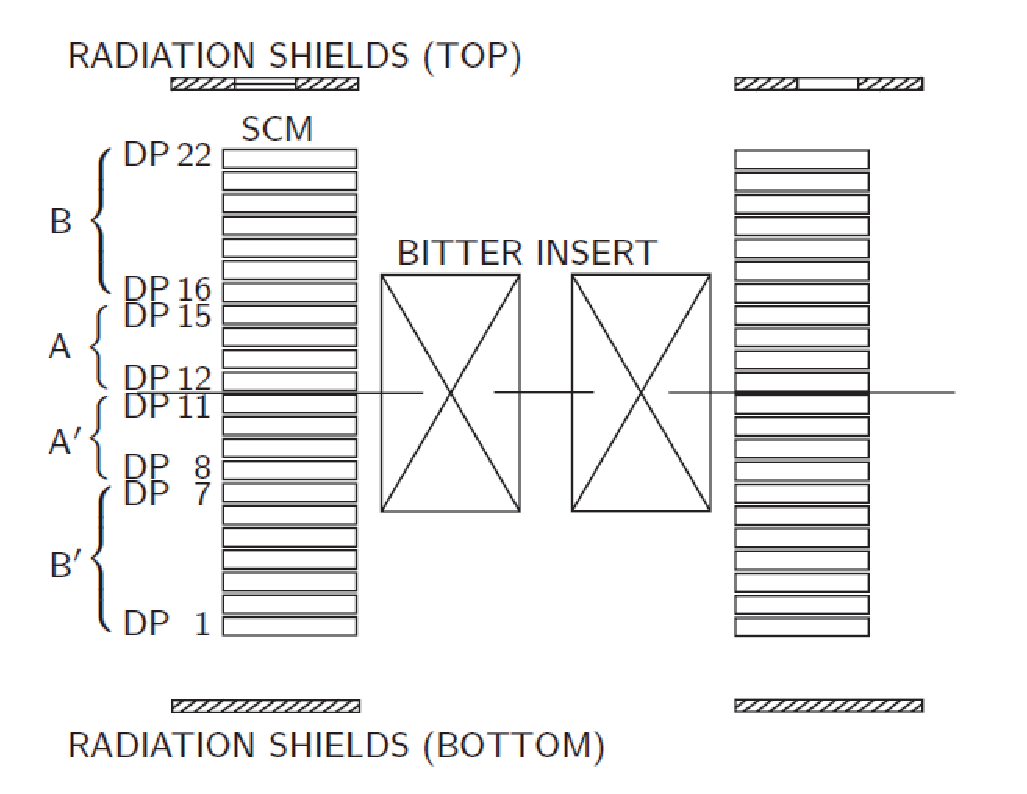
\includegraphics[scale=0.6]{chpt8/figs/fig8.20.eps}
	\caption{混合II磁体的结果示意图,包括Bitter内插磁体,22个双饼超导磁体和辐射屏蔽板。}
\end{figure}

\textbf{A. 技术I}

本技术中,磁体被分为两组:A+A'和B+B'。
本技术相比传统技术将磁体分为B'+A'和B+A,能更好的消除电感电压,但仍不能完全令人满意。
本技术不能消除水冷磁体或NbTi线圈励磁时的全部的电感电压。

\textbf{B. 技术II}

由Ishigohka[8.114]提出的第二种技术所有22个双饼上的电压抽头,将他们组合成两个主要部分:
一部分包括偶数双饼,$V_{2n-1}(t)$;另一部分包括奇数双饼,$V_{2n}(t)$。
通过调整22个独立放大器的增益,可以在没有电阻性电压的情况下调节各双饼的电压以最小化$V_{out}(t)$。于是:
\begin{equation}% 8.75
V_{out}(t)=\sum_{n=1}^{11}[\alpha_{2n-1}V_{2n-1}(t)-\alpha_{2n}V_{2n}(t)]
\end{equation}
式中,$\alpha_{2n-1}$是第$(2n-1)^{th}$个双饼的放大器增益,
$\alpha_{2n}$是第$(2n)^{th}$个双饼的放大器增益。

使用技术I消除感性电压的成功与否取决于两部分的与电流水平或电流变化率无关电感电压的接近程度。
混合II中,因为容纳NbTi的低温容器并不关于线圈中平面对称,
电压平衡不能做到与电流水平或电流变化率无关。

同时,更严重的,单独针对NbTi线圈充电优化的电桥在插入磁体充电时不再最优,
优化的设置随自场变化率和内插磁体变化率而变化。

技术II极大的减小了包括超导线圈、内插磁体、辐射屏蔽板和低温容器其他部件在内的整个系统的不对称性。
这令总不平衡感性电压比那些中平面/末端条件下的电压有数量级的下降。

图8.21给出了25 kA[8.114]下插入内插磁体下的3个平衡电压$V_{AA'},V_{BB'}$和奇偶差分电压$V_{\delta}$
可以看到,$V_{BB'}-V_{AA'}$比$V_\delta$的峰值大100倍以上。

于是,$V_\delta$仅在检测超导线圈运行条件时是一个更敏感的方法。
提高敏感性的代价是需要大量的差分放大器,并且要求每一个都不能失效。

\begin{figure}
	\centering
	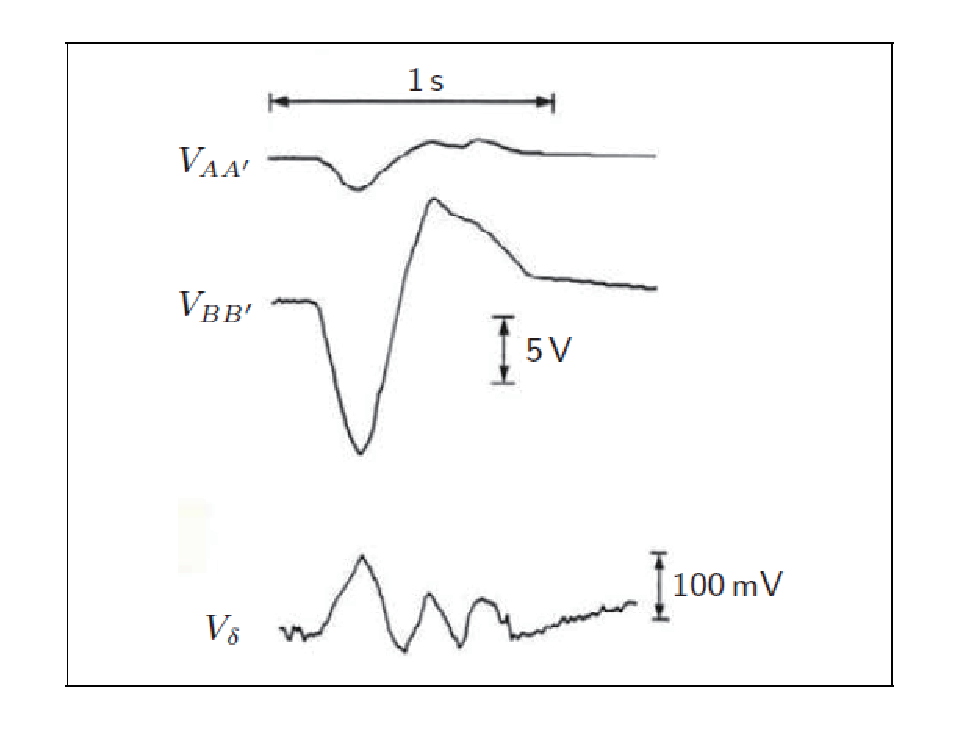
\includegraphics[scale=0.6]{chpt8/figs/fig8.21.eps}
	\caption{混合II磁体在内插磁体时测到不平衡电压。}
\end{figure}


\subsection{问题8.5:泄放电阻的设计}
在这里,我们研究主动保护中使用的泄放电阻$R_D$的设计标准[8.115,8.116]。
 两个参数很重要:1) $R_D$本身的值; 2) 储能$E_m$。
  $E_m$之所以重要,是因为在几乎每个泄放电阻都必须吸收$E_m$的大部分;
   显然,谨慎的设计假设是100\%的$E_m$被电阻器绝热吸收。 
   如图8.22所示,这里让我们假设我们的电阻是一个长条形,长$\ell$,截面为矩形,宽$w$,厚$\delta$。
   
由于泄放电阻经常承受远高于100 V的泄放电压且吸收的能量远大于1 MJ,
在加热到200 K甚至高于室温的过程中,必须慎重选择其在磁体系统中位置,其中,安全是最重要的标准。
泄放电阻通常放置在有围栏的隔离区域,以使其远离人员和其他设备。

a) 证明电阻器的长度$\ell$为:
\begin{equation}% 8.76a
\ell=\sqrt{\frac{E_mR_D}{\rho C_p\Delta T}}
\end{equation}
其中,$\rho$是电阻器材料(通常是钢)的电阻率。
因为电阻器绝热吸收$E_m$,它的温度显然会升高。
$C_p$是电阻器材料的热容,假设为常数。在这里是一个可以接受的界定,特别是在300 K以上的温区。
$\Delta T$是电阻器在绝热吸收$E_m$后的总温升。

b) 证明导体的横截面应为:
\begin{align*}% 8.76b
\omega\delta=\sqrt{\frac{\rho E_m}{R_DC_p\Delta T}} \tag{8.76b}
\end{align*}
$\ell$和$w\delta$对这些参数的依赖性容易理解。

c) 计算混合III参数下的$\ell$和$w\delta$:
$E_m\simeq$20 MJ;$R_D=0.3\ \Omega$;
对钢,有$\rho\simeq10^{-6}\ \Omega$m,$C_p\simeq 4\times 10^6\ \mathrm{J/m^2K}$;以及
$\Delta T\simeq$200 K。
\begin{figure}
	\centering
	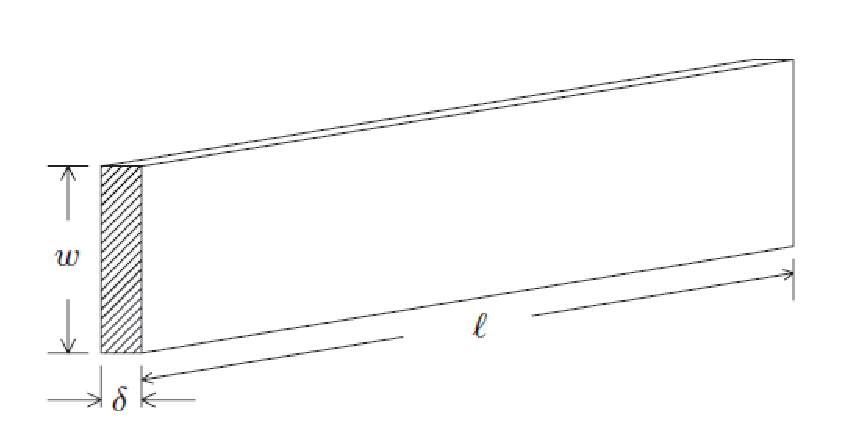
\includegraphics[scale=0.6]{chpt8/figs/fig8.22.eps}
	\caption{长条泄放电阻器的示意图。长$\ell$,截面为$w\delta$。}
\end{figure}

\subsubsection{问题8.5之解}
a) 泄放电阻的$R_D$由下式给出:
\begin{align*}% page518 S5.1a
R_D-\frac{\rho\ell}{\omega\delta} \tag{S5.1a}
\end{align*}
或
\begin{align*}% page518 S5.1b
\omega\delta=\frac{\rho\ell}{R_D} \tag{S5.1b}
\end{align*}

绝热吸收的$E_m$令电阻升温$\Delta T$:
\begin{align*}% page518 S5.2a
E_m=\ell\omega\delta C_p\Delta T \tag{S5.2a}
\end{align*}
或
\begin{align*}% page518 S5.2b
\omega\delta=\frac{E_m}{\ell C_p\Delta T} \tag{S5.2b}
\end{align*}

令S5.1b和S5.2b相等,解出$\ell$,有:
\begin{align*}% 8.76a
\omega\delta=\sqrt{\frac{\rho E_m}{R_DC_p\Delta T}} \tag{8.76a}
\end{align*}

b)将8.76a给出的$\ell$代入S5.1b,得到:
\begin{align*}
w\delta=\sqrt{\frac{\rho E_m}{R_D C_p \Delta T}} \tag{8.76b}
\end{align*}

c) 我们计算混合III磁体的$\ell$和$w\delta$,有:
\begin{align*}
\ell&\simeq\sqrt{\frac{(2\times 10^7\ \mathrm{J})(0.3\Omega)}{(10^{-6}\ \mathrm{\Omega m})(4\times 1066\ \mathrm{J/m^2K})(200\ \mathrm{K})}} \\
&=86.6\ \mathrm{m}\\
\omega\delta&\simeq\sqrt{\frac{(10^{-6}\ \mathrm{\Omega m})(2\times 10^7\ \mathrm{J})}{(0.3\Omega)(4\times 10^6\ \mathrm{J/m^2K})(200\ \mathrm{K})}} \\
&\simeq 2.9\times 10^{-4}\ \mathrm{m^2}\simeq 290\ \mathrm{mm^2}
\end{align*}

混合III磁体的泄放电阻器包括电气上串联的近90个钢条,
每根长约1 m,宽约5 cm,厚6 mm。
如果$\Delta T$被限定于100 K,$\ell$和$w\delta$将增加约40\%:
$\ell\simeq$120 m,$w\delta\simeq 410\ \mathrm{mm^2}$ 。


\subsection{讨论8.2:磁体的“缓慢”放电模式}
\begin{equation}% 8.77a
\frac{dI_m(t)}{dt}=-\frac{I_m(t)}{\tau_m}
\end{equation}


\begin{figure}
	\centering
	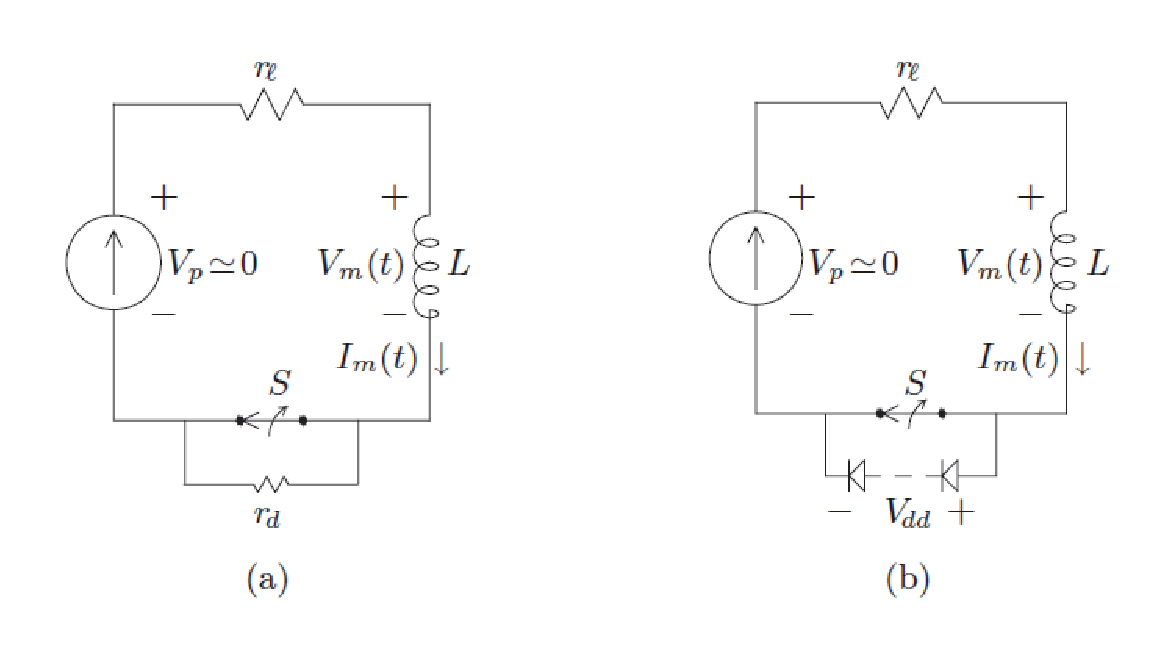
\includegraphics[scale=0.6]{chpt8/figs/fig8.23.eps}
	\caption{Circuits for “slow” discharge modes: (a}
\end{figure}






\begin{equation}% 8.77b
\frac{dI_m(t)}{dt}=-\frac{V_{dd}}{L}
\end{equation}


\subsection{讨论8.3:低阻电阻器设计}
\begin{equation}% 8.78a
r_d=\frac{\rho\ell}{\omega\delta}
\end{equation}
\begin{equation}% 8.78b
r_dI_m(0)^2\simeq 2\omega\ell g_{cv}
\end{equation}
\begin{equation}% 8.79a
\ell\simeq r_dI_m(0)\sqrt{\frac{\delta}{2\rho g_{cv}}}
\end{equation}
\begin{equation}% 8.79b
\omega\simeq I_m(0)\sqrt{\frac{\rho}{2\delta g_{cv}}}
\end{equation}
\begin{equation}% page521 第一个
\ell\simeq(0.01\Omega)(250\ \mathrm{A})\sqrt{\frac{(250\times 10^{-6}\ \mathrm{m})}{2(10^{-6}\ \mathrm{\Omega m})(20\ \mathrm{W/m^2})}} 
\simeq 6.3\ \mathrm{m}
\end{equation}
\begin{equation}% page521 第二个
\omega\simeq(250\ \mathrm{A})\sqrt{\frac{(10^{-6}\ \mathrm{\Omega m})}{2(250\times 10^{-6}\ \mathrm{m})(20\ \mathrm{W/m^2})}} 
\simeq 2.5\ \mathrm{m}
\end{equation}
\begin{equation}% page521第三个
\ell\simeq(0.01\Omega)(250\ \mathrm{A})\sqrt{\frac{(250\times 10^{-6}\ \mathrm{m})}{2(10^{-6}\ \mathrm{\Omega m})(20\times 10^3\ \mathrm{W/m^2})}} 
\simeq 20\ \mathrm{cm}
\end{equation}
\begin{equation}% page521 第四个
\omega\simeq(250\ \mathrm{A})\sqrt{\frac{(10^{-6}\ \mathrm{\Omega m})}{2(250\times 10^{-6}\ \mathrm{m})(20\times 10^3\ \mathrm{W/m^2})}} 
\simeq 8\ \mathrm{cm}
\end{equation}


\subsection{讨论8.4:过热\& 内部电压判据}

\begin{align*}% page522 8.30a
J_{m_{op}}^{sh}&=\left(\frac{1+\gamma_{m/s}}{\gamma_{m/s}}\right)\frac{f_r\pi(\alpha+1)\rho_m(T_f)Z(T_f,T_i)}{2}\sqrt{\frac{a_1}{2\mu_o\ \mathcal{L}(\alpha,\beta)E_m}} \\
&=\left(\frac{1+1}{1}\right)\frac{(0.5)\pi(1.3+1)(1.11\times 10^{-8}\ \mathrm{\Omega m})(10.5\times 10^{16}\ \mathrm{A^2s/m^4})}{2}\times \\
&=\sqrt{\frac{0.15\ \mathrm{m}}{2(4\pi\times 10^{-7}\ \mathrm{H/m})(0.54)(3\times 10^6\ \mathrm{J})}} \\
&\simeq 2(21.1\times 10^8\ \mathrm{J/m^3})(0.19\ \mathrm{Am/J})\\
&\simeq 805\ \mathrm{MA/m^2}=805\ \mathrm{A/mm^2}
\end{align*}



\begin{align*}% 8.40b
J_{m_{op}}^{V}&=\frac{2}{f_r(1-f_r)}\left[\frac{\sqrt{\mathcal{L}(\alpha,\beta)}}{\pi(\alpha+1)}\right]\left[\frac{V_{bk}I_{op}}{\rho_m(T_f)}\sqrt{\frac{2\mu_o}{a_1E_m}}\right] \\
&=\frac{2}{0.5(1-0.5)}\left[\frac{\sqrt{0.54}}{\pi(1.3+1)}\right]\left[\frac{(10^4\ \mathrm{V})(300\ \mathrm{A})}{(1.11\times 10^{-8}\ \mathrm{\Omega m})}\sqrt{\frac{2(4\pi\times 10^{-7}\ \mathrm{H/m})}{(0.15\ \mathrm{m})(3\times 10^6\ \mathrm{J})}}\right] \\
&=8(0.102)(2.70\times 10^{14}\ \mathrm{A^2/m})(2.36\times 10^{-6}\ \mathrm{A^{-1}m^{-1}}) \\
&=5.2\times 10^8\ \mathrm{A/m^2}=520\ \mathrm{A/mm^2}
\end{align*}


\subsection{讨论8.5:Bi2223带电流引线的保护}

\begin{equation}% 8.80
a_mk_m\frac{d^2T}{dz^2}+\frac{\rho_mI_{t}^{2}}{a_m}=0
\end{equation}
\begin{equation}% 8.81
T(\zeta)=T_{cl}+(T_{wm}-T_{cl})\zeta+\frac{\rho_m\ell^2I_{t}^{2}}{2a_{m}^{2}k_m}(\zeta-\zeta^2)
\end{equation}
\begin{equation}% 8.82a
\zeta(T_{pk})=\frac{1}{2}+\frac{a_{m}^{2}k_m}{\rho_mI_{t}^{2}\ell^2}(T_{wm}-T_{cl})
\end{equation}
\begin{equation}% 8.82b
T_{pk}\simeq \frac{1}{2}(T_{cl}+T_{wm})+\frac{\rho_mI_{t}^{2}\ell^2}{8a_{m}^{2}k_m}
\end{equation}
\begin{equation}% page523 最后一个
\frac{a_{m}^{2}k_m}{\rho_mI_{t}^{2}\ell^2}(T_{wm}-T_{cl})=\frac{(8\times 10^{-3}\ \mathrm{cm^2})^2(2\ \mathrm{W/cm K})}{(1\times 10^{-6}\ \mathrm{\Omega cm})(50\ \mathrm{A})^2(15\ \mathrm{cm})^2} 
\simeq 0.01
\end{equation}
\begin{equation}% page524 第一个
T_{pk}\simeq\frac{1}{2}(T_{cl}+\frac{\rho_mI_{t}^{2}\ell^2}{8a_{m}^{2}k_m} 
=\frac{1}{2}(10\ \mathrm{K}+70\ \mathrm{K})+\frac{(1\times 10^{-6}\ \mathrm{\Omega cm})(50\ \mathrm{A})^2(15\ \mathrm{cn})^2}{8(8\times 10^{-3}\ \mathrm{cm^2})^2(2\ \mathrm{W/cm K})}\simeq 590\ \mathrm{K}
\end{equation}



\subsection{讨论8.6:$MgB_2$磁体的主动保护}



\begin{figure}
	\centering
	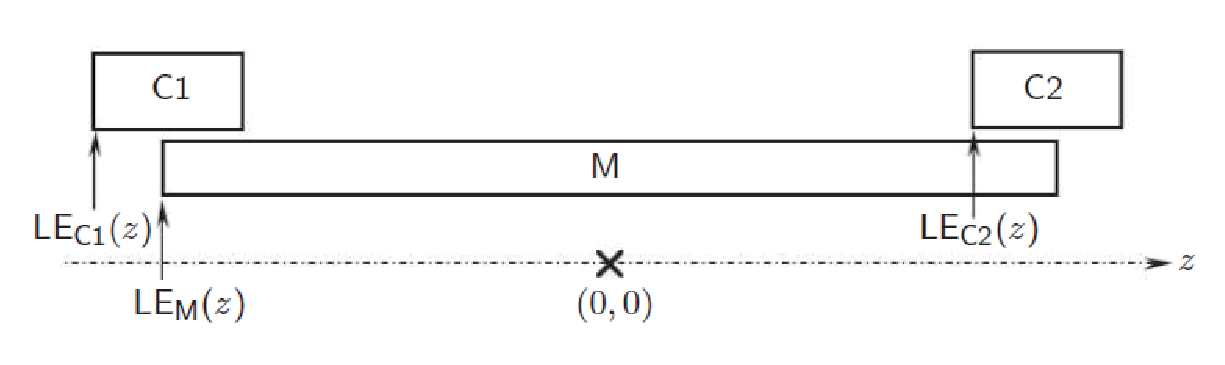
\includegraphics[scale=0.6]{chpt8/figs/fig8.24.eps}
	\caption{Schematic drawing of a magnet comprised of three solenoids}
\end{figure}


\begin{figure}
	\centering
	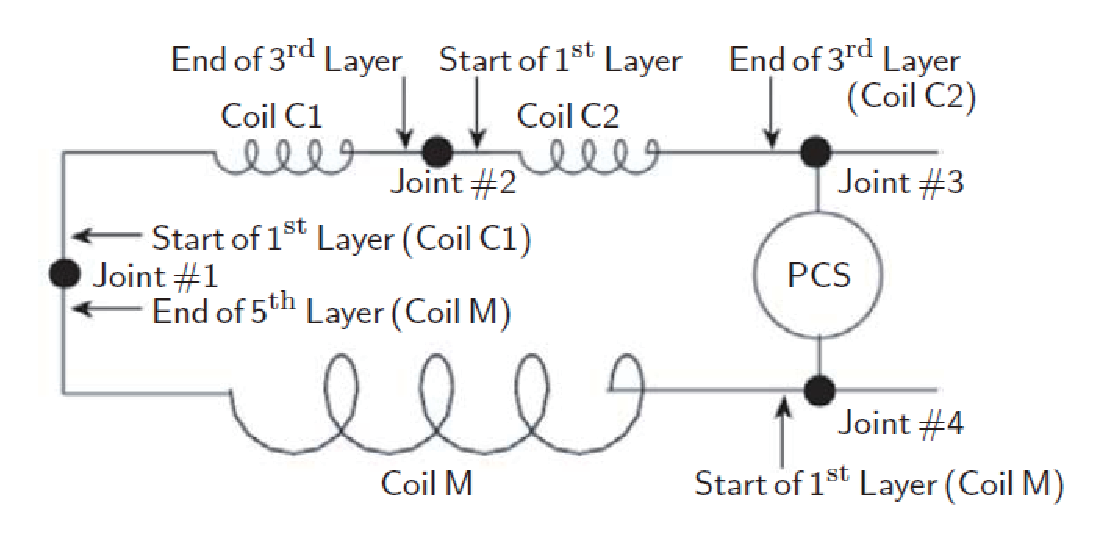
\includegraphics[scale=0.6]{chpt8/figs/fig8.25.eps}
	\caption{Schematic drawing of a 3-coil arrangement, shunted by PCS for persistent}
\end{figure}




\begin{equation}% page528 8.9c
\int_{T_i}^{T_f}\frac{C_m(T)}{\rho_m(T)}dT=\left(\frac{A_m}{A_{cd}}\right)J_{m_o}^{2}\tau_{ah}
\end{equation}
\begin{equation}% page528 6.33
R_{mz}=\sqrt{\frac{3k_{wd}(T_c-T_{op})}{\rho_mJ_{m}^{2}}}
\end{equation}
\begin{equation}% 8.83a
V_M(t)=V_r(t)+(L_M+M_{MC1}+M_{MC2})\frac{dI_{op}(t)}{dt}
\end{equation}
\begin{equation}% 8.83b
V_{C1}(t)=(L_{C1}+M_{C1M}+M_{C1C2})\frac{dI_{op}}{dt}=V_{C2}(t)=-\frac{1}{2}V_M(t)
\end{equation}
\begin{equation}% 8.83c
V_M(t)+V_{C1}(t)+V_{C2}(t)=0
\end{equation}



\subsection{问题8.6:NMR磁体的被动保护}


\begin{figure}
	\centering
	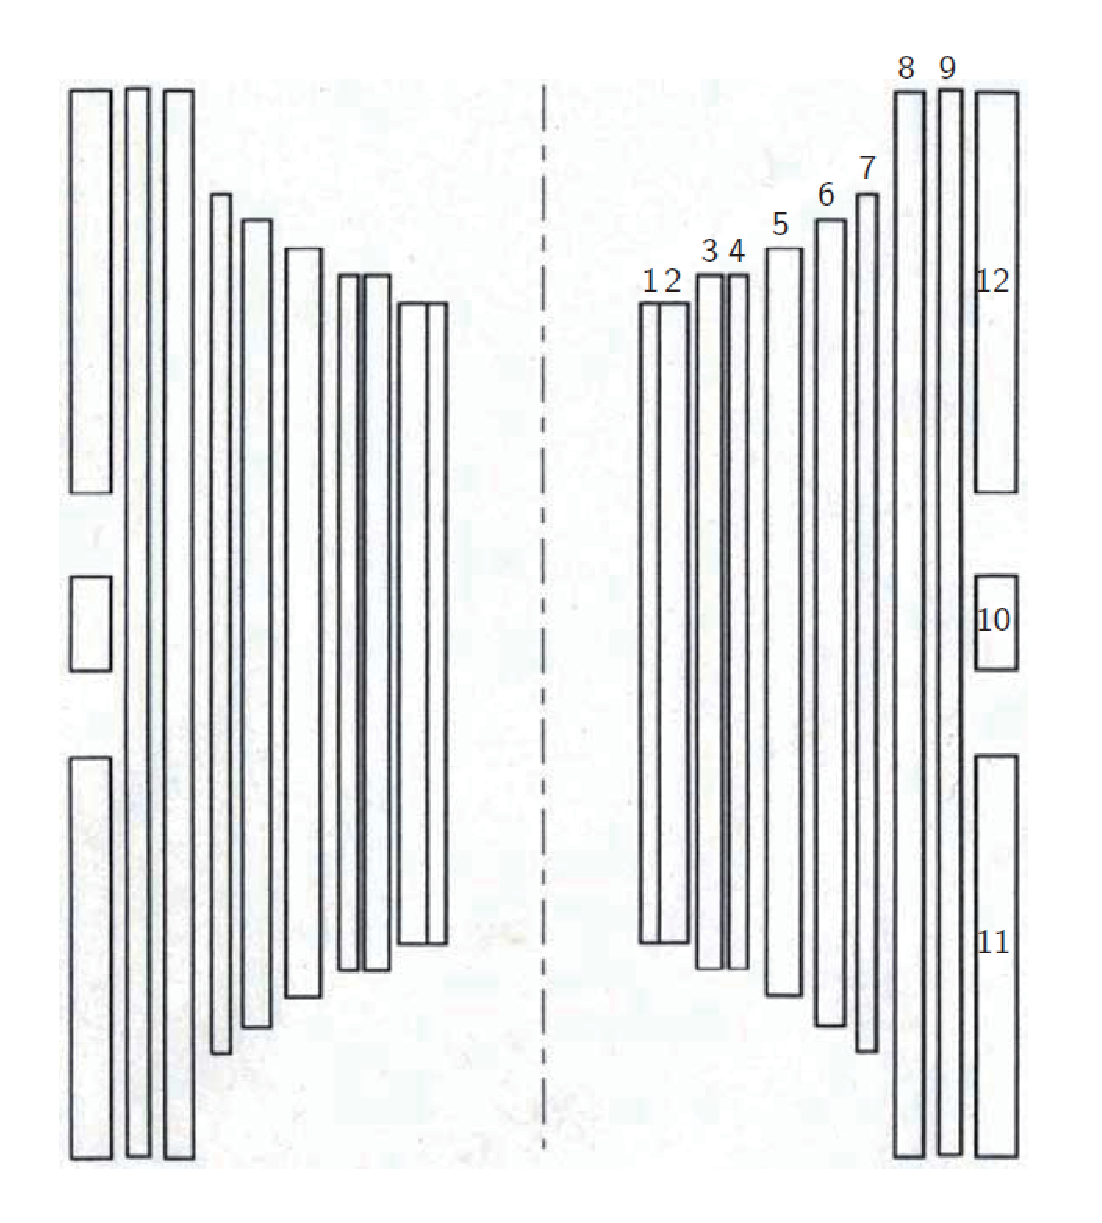
\includegraphics[scale=0.6]{chpt8/figs/fig8.26.eps}
	\caption{Drawing showing the locations of 12 coils in }
\end{figure}


\begin{figure}
	\centering
	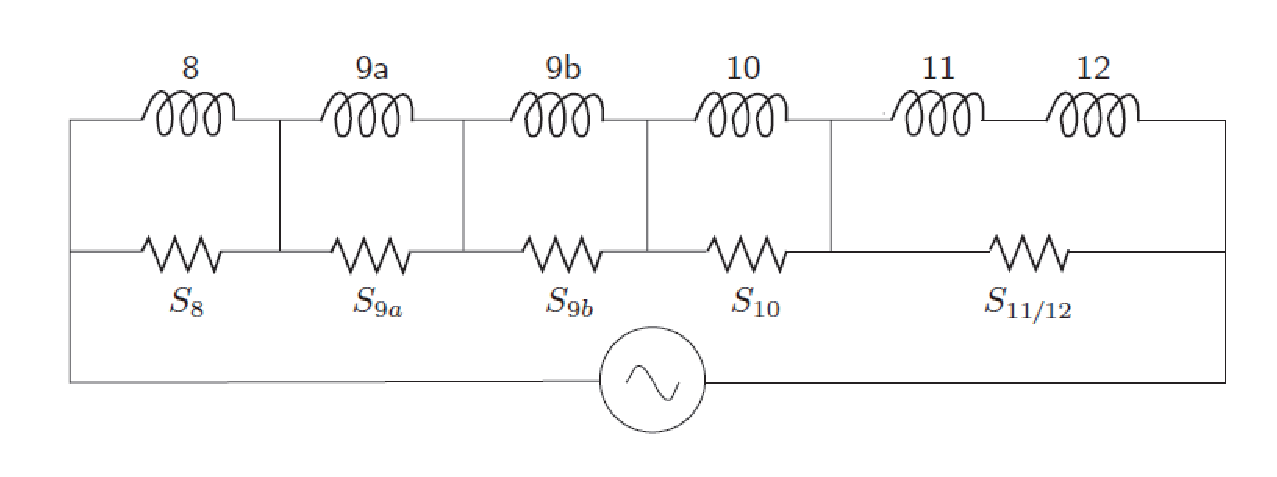
\includegraphics[scale=0.6]{chpt8/figs/fig8.27.eps}
	\caption{Circuit for the NbTi coils}
\end{figure}


\begin{figure}
	\centering
	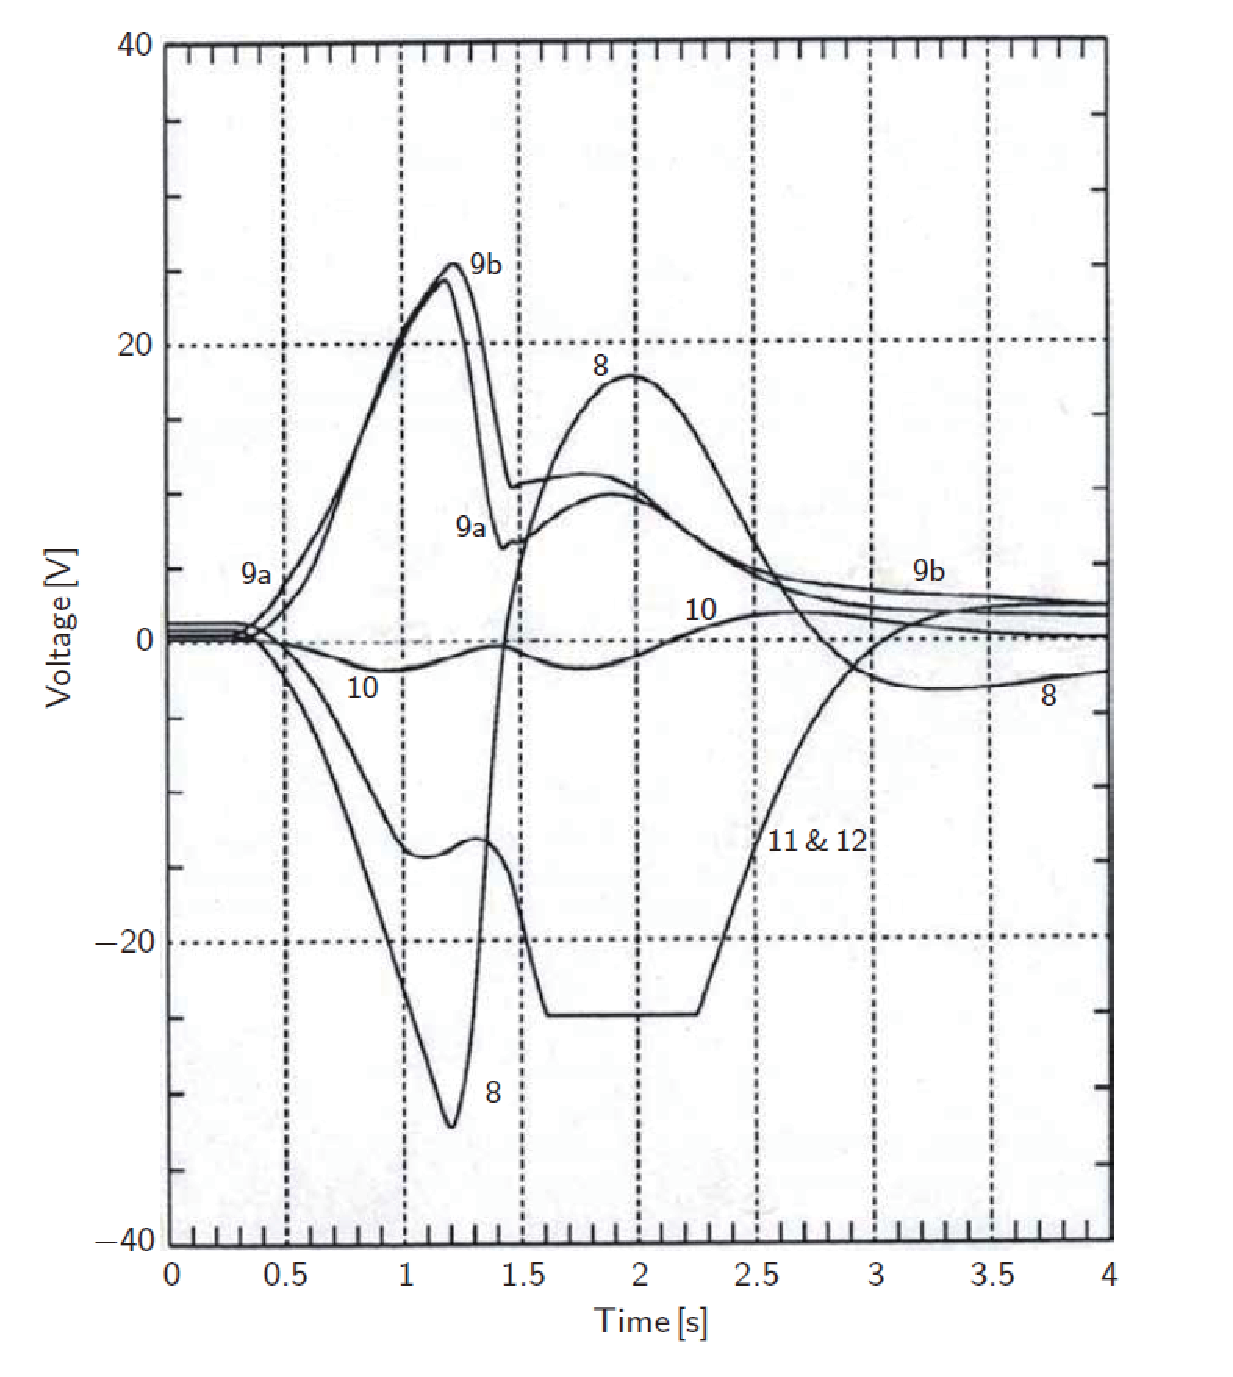
\includegraphics[scale=0.6]{chpt8/figs/fig8.28.eps}
	\caption{Voltage traces recorded acro}
\end{figure}


\begin{figure}
	\centering
	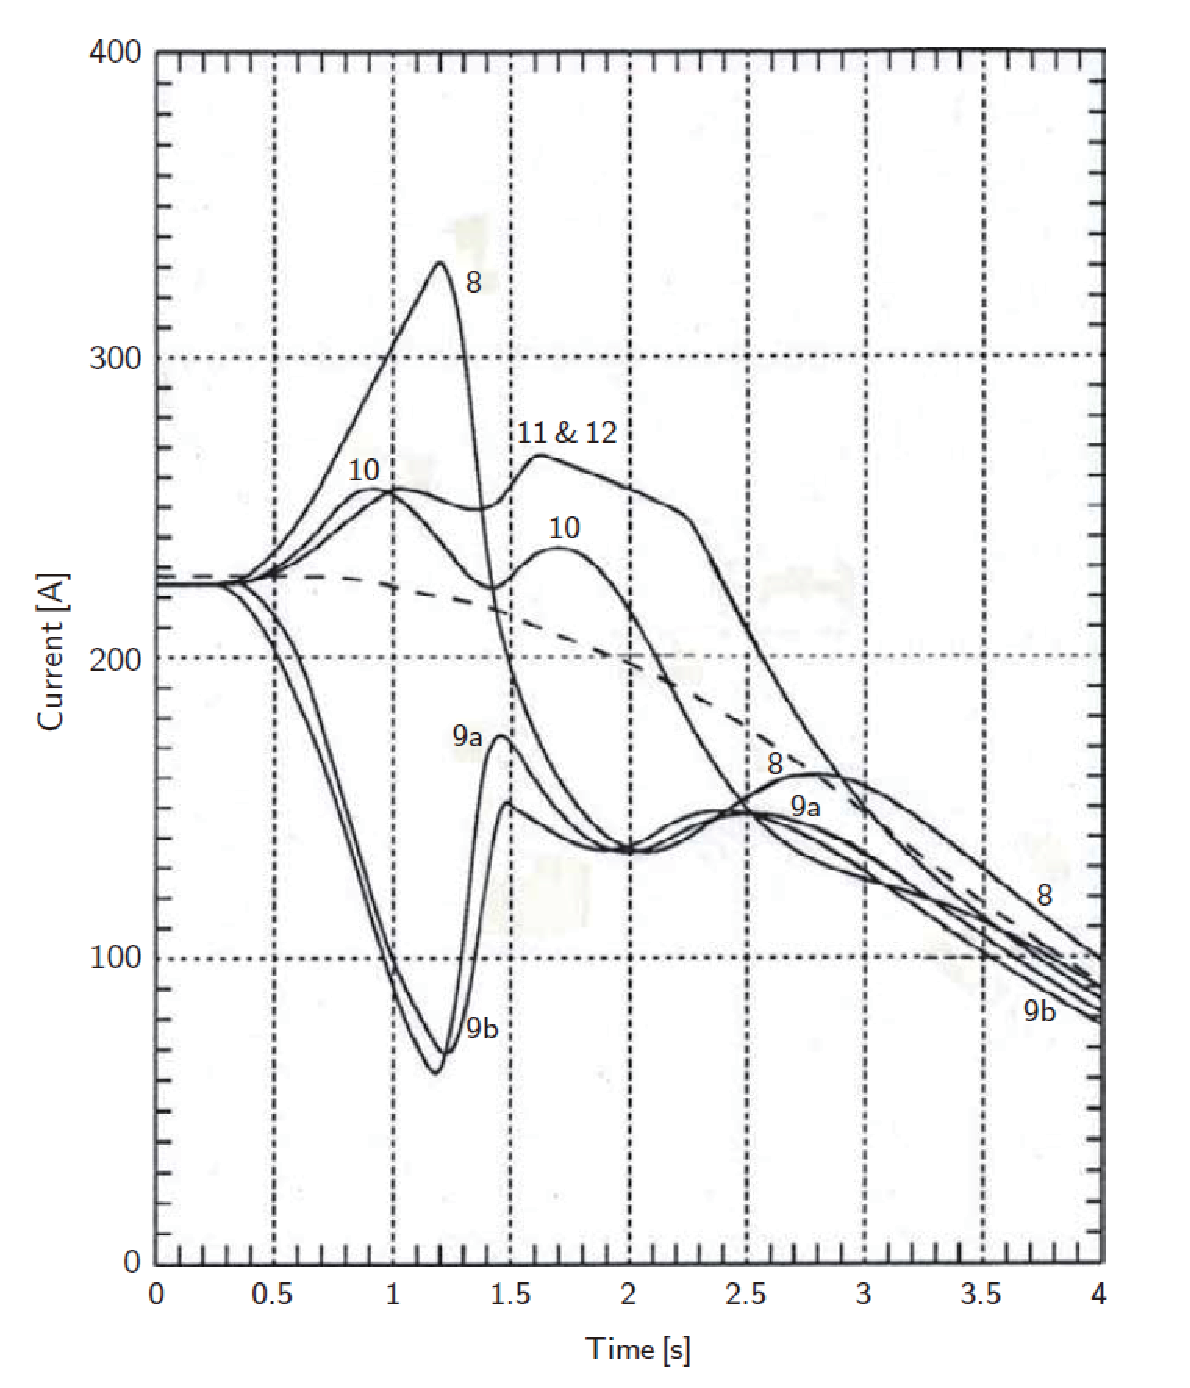
\includegraphics[scale=0.6]{chpt8/figs/fig8.29.eps}
	\caption{Current traces through Coils 8, 9a, 9b, 10, and 11/12 corresponding}
\end{figure}



\begin{equation}% 8.84a
I_8=I_0-\frac{V_8}{S_8}
\end{equation}
\begin{equation}% 8.84b
I_{9a}=I_0-\frac{V_{9a}}{S_{9a}}
\end{equation}
\begin{equation}% 8.84c
I_{9b}=I_0-\frac{V_{9b}}{S_{9b}}
\end{equation}
\begin{equation}% 8.84d
I_{10}=I_0-\frac{V_{10}}{S_{10}}
\end{equation}
\begin{equation}% 8.84e
I_{11/12}=I_0\frac{V_{11/12}}{S_{11/12}}
\end{equation}


\subsubsection{问题8.6之解}

\begin{equation}% page535 8.84a
I_8=I_0-I_{r8}  
=I_0-\frac{V_8}{S_8}
\end{equation}
\begin{equation}% page535 8.84b
I_{9a}=I_8+I_{r8}-I_{r9a}=I_0-\frac{V_8}{S_8}+\frac{V_8}{S_8}-\frac{V_{9a}}{S_{9a}}
=I_0-\frac{V_{9a}}{S_{9a}}
\end{equation}
\begin{equation}% page535 8.84c
I_{9b}=I_{9a}+\frac{V_{9a}}{S_{9a}}-\frac{V_{9b}}{S_{9b}}=I_0-\frac{V_{9a}}{S_{9a}}+\frac{V_{9a}}{S_{9a}}-\frac{V_{9b}}{S_{9b}} 
=I_0\frac{V_{9b}}{S_{9b}}
\end{equation}
\begin{equation}% page535 8.84d
I_{10}=I_{9b}+\frac{V_{9b}}{S_{9b}}-\frac{V_{10}}{S_{10}}=I_0-\frac{V_{9b}}{S_{9b}}+\frac{V_{9b}}{S_{9b}}-\frac{V_{10}}{S_{10}}
=I_0-\frac{V_{10}}{S_{10}}
\end{equation}
\begin{equation}% page535 8.84e
I_{11/12}=I_{10}+\frac{V_{10}}{S_{10}}-\frac{V_{11/12}}{S_{11/12}}=I_0-\frac{V_{10}}{S_{10}}+\frac{V_{10}}{S_{10}}-\frac{V_{11/12}}{S_{11/12}}
=I_0-\frac{V_{11/12}}{S_{11/12}}
\end{equation}
\begin{equation}% page535 S6.1
V_8=V_r\mid_8+L_8\frac{dI_8}{dt}+M_{8,9a}\frac{dI_{9a}}{dt}+M_{8,9b}\frac{dI_{9b}}{dt} 
+M_{8,10}\frac{dI_{10}}{dt}+M_{8,11}\frac{dI_{11}}{dt}+M_{8,12}\frac{dI_{12}}{dt}
\end{equation}
\begin{equation}% page535 S6.2a
V_8\simeq V_r\mid_8+(4.413\ \mathrm{H})(84.5\ \mathrm{A/s})+(2.268\ \mathrm{H})(-154.1\ \mathrm{A/s}) 
+(2.243\ \mathrm{H})(-107.1\ \mathrm{A/s})+(0.715\ \mathrm{H})(41.3\ \mathrm{A/s}) 
+(2.747\ \mathrm{H})(33.6\ \mathrm{A/s})+(2.755\ \mathrm{H})(33.6\ \mathrm{A/s})
\end{equation}
\begin{equation}% page535 S6.2b
V_8=V_r\mid_8+372.9-349.5-240.2+39.4+92.4+92.6 
=V_r\mid_8-2.5\ \mathrm{V}
\end{equation}
\begin{equation}% page536 S6.3a
V_8=V_r\mid_8+(4.413\ \mathrm{H})(147.2\ \mathrm{A/s})+(2.268\ \mathrm{H})(-234.7\ \mathrm{A/s}) 
+(2.243\ \mathrm{H})(-198.1\ \mathrm{A/s})+(0.715\ \mathrm{H})(-44.8\ \mathrm{A/s}) 
+(2.747\ \mathrm{H})(19.3\ \mathrm{A/s})+(2.755\ \mathrm{H})(19.3\ \mathrm{A/s})
\end{equation}
\begin{equation}% page536 S6.3b
V_8=V_r\mid_8+(649.6-532.3-444.3-32.0+53.0+53.2)[\mathrm{V}]
=V_r\mid_8-252.9[\mathrm{V}]
\end{equation}
\begin{equation}% page536 S6.4
P_{mg}=\sum_{n=8}^{12}V_r\mid_n\times I_n
\end{equation}
\begin{equation}% page536 S6.5
P_{mg}\simeq\left(\tilde{V}-\sum_{m,n=8}^{12}L_{m,n}\frac{d\tilde{I}}{dt}\right)\times \tilde{I}
\end{equation}
\begin{equation}% page536 S6.6
P_{mg}\simeq[0-(60.25\ \mathrm{H})(-50\ \mathrm{A/s})](90\ \mathrm{A})\simeq 270,000\ \mathrm{W}
\end{equation}




\subsection{讨论8.7:HTS磁体到底要不要保护?}
\begin{equation}% 8.85a
\$_{T/w}=\$_M+\$_{qp}
\end{equation}
\begin{equation}% 8.85b
\$_{T/wo}=\$_M+P_{dm}(\$_M+\$_{ra})
\end{equation}